\documentclass[a4paper,11pt]{book}
%\documentclass[a4paper,twoside,11pt,titlepage]{book}
\usepackage{listings}
\usepackage[utf8]{inputenc}
\usepackage[spanish]{babel}
\usepackage{multirow}
% \usepackage[style=list, number=none]{glossary} %
%\usepackage{titlesec}
%\usepackage{pailatino}
% \DeclareUnicodeCharacter{22C6}{*************************************}

\decimalpoint
\usepackage{dcolumn}
\newcolumntype{.}{D{.}{\esperiod}{-1}}
\makeatletter
\addto\shorthandsspanish{\let\esperiod\es@period@code}
\makeatother


%\usepackage[chapter]{algorithm}
\RequirePackage{verbatim}
%\RequirePackage[Glenn]{fncychap}
\usepackage{fancyhdr}
\usepackage{graphicx}
\usepackage{afterpage}

\usepackage{longtable}

\usepackage{colortbl, longtable}
\usepackage[table,xcdraw]{xcolor}


\usepackage[pdfborder={000}]{hyperref} %referencia

% ********************************************************************
% Re-usable information
% ********************************************************************
\newcommand{\myTitle}{Título del proyecto\xspace}
\newcommand{\myDegree}{Máster en Ingeniería Informática\xspace}
\newcommand{\myName}{Andrea Morales Garzón (alumno)\xspace}
\newcommand{\myProf}{Nombre Apllido1 Apellido2 (tutor1)\xspace}
\newcommand{\myOtherProf}{Nombre Apllido1 Apellido2 (tutor2)\xspace}
%\newcommand{\mySupervisor}{Put name here\xspace}
\newcommand{\myFaculty}{Escuela Técnica Superior de Ingenierías Informática y de
Telecomunicación\xspace}
\newcommand{\myFacultyShort}{E.T.S. de Ingenierías Informática y de
Telecomunicación\xspace}
\newcommand{\myDepartment}{Departamento de ...\xspace}
\newcommand{\myUni}{\protect{Universidad de Granada}\xspace}
\newcommand{\myLocation}{Granada\xspace}
\newcommand{\myTime}{\today\xspace}
\newcommand{\myVersion}{Version 0.1\xspace}


\hypersetup{
pdfauthor = {\myName (email (en) ugr (punto) es)},
pdftitle = {\myTitle},
pdfsubject = {},
pdfkeywords = {palabra_clave1, palabra_clave2, palabra_clave3, ...},
pdfcreator = {LaTeX con el paquete ....},
pdfproducer = {pdflatex}
}

%\hyphenation{}
\definecolor{UniBlue}{RGB}{2,59,183}
\definecolor{myGreen}{RGB}{67,207,1}
\definecolor{myRed}{RGB}{200,1,40}

%\usepackage{doxygen/doxygen}
%\usepackage{pdfpages}
\usepackage{url}
\usepackage{colortbl,longtable}
\usepackage[stable]{footmisc}
\usepackage{index}


\usepackage{biblatex} %Imports biblatex package
\addbibresource{sample.bib} %Import the bibliography file
\usepackage{pifont}
\usepackage{amssymb}
\newcommand{\cmark}{\ding{52}}%
\newcommand{\xmark}{\ding{56}}%




\makeindex
%\usepackage[style=long, cols=2,border=plain,toc=true,number=none]{glossary}
%\makeglossary

% Definición de comandos que me son tiles:
%\renewcommand{\indexname}{Índice alfabético}
%\renewcommand{\glossaryname}{Glosario}

\pagestyle{fancy}
\fancyhf{}
\fancyhead[LO]{\leftmark}
\fancyhead[RE]{\rightmark}
\fancyhead[RO,LE]{\textbf{\thepage}}
\renewcommand{\chaptermark}[1]{\markboth{\textbf{#1}}{}}
\renewcommand{\sectionmark}[1]{\markright{\textbf{\thesection. #1}}}

\setlength{\headheight}{1.5\headheight}

\newcommand{\HRule}{\rule{\linewidth}{0.5mm}}
%Definimos los tipos teorema, ejemplo y definición podremos usar estos tipos
%simplemente poniendo \begin{teorema} \end{teorema} ...
\newtheorem{teorema}{Teorema}[chapter]
\newtheorem{ejemplo}{Ejemplo}[chapter]
\newtheorem{definicion}{Definición}[chapter]

\definecolor{gray97}{gray}{.97}
\definecolor{gray75}{gray}{.75}
\definecolor{gray45}{gray}{.45}
\definecolor{gray30}{gray}{.94}
\definecolor{airforceblue}{rgb}{0.36, 0.54, 0.66}
\definecolor{arsenic}{rgb}{0.23, 0.27, 0.29}
\definecolor{blue(munsell)}{rgb}{0.0, 0.5, 0.69}
\definecolor{bondiblue}{rgb}{0.0, 0.58, 0.71}
\definecolor{bluegray}{rgb}{0.4, 0.6, 0.8}
\definecolor{cadet}{rgb}{0.23, 0.41, 0.67}
\definecolor{britishracinggreen}{rgb}{0.0, 0.26, 0.15}
\definecolor{oldrose}{rgb}{0.75, 0.5, 0.51}
\definecolor{oldmauve}{rgb}{0.4, 0.19, 0.28}
\definecolor{pastelgray}{rgb}{0.81, 0.81, 0.77}
\definecolor{gray15}{gray}{.30}
\definecolor{gray(x11gray)}{rgb}{0.97, 0.97, 0.97}
\definecolor{mygray}{rgb}{0.5,0.5,0.5}
\definecolor{codegreen}{rgb}{0,0.6,0}
\definecolor{codegray}{rgb}{0.5,0.5,0.5}
\definecolor{codepurple}{rgb}{0.58,0,0.82}
\definecolor{backcolour}{rgb}{0.95,0.95,0.92}



\usepackage{comment}

\lstset{ frame=Ltb,
     framerule=0.5pt,
     aboveskip=0.5cm,
     framextopmargin=3pt,
     framexbottommargin=3pt,
     framexleftmargin=0.1cm,
     framesep=0pt,
     rulesep=.4pt,
     backgroundcolor=\color{gray97},
     rulesepcolor=\color{black},
     %
     stringstyle=\ttfamily,
     showstringspaces = false,
     basicstyle=\scriptsize\ttfamily,
     commentstyle=\color{gray45},
     keywordstyle=\bfseries,
     %
     numbers=left,
     numbersep=6pt,
     numberstyle=\tiny,
     numberfirstline = false,
     breaklines=true,
   }
 
% minimizar fragmentado de listados
\lstnewenvironment{listing}[1][]
   {\lstset{#1}\pagebreak[0]}{\pagebreak[0]}

\lstdefinestyle{CodigoC}
   {
	basicstyle=\scriptsize,
	frame=single,
	language=C,
	numbers=left
   }
\lstdefinestyle{CodigoC++}
   {
	basicstyle=\small,
	frame=single,
	backgroundcolor=\color{gray30},
	language=C++,
	numbers=left
   }

 
\lstdefinestyle{Consola}
   {basicstyle=\scriptsize\bf\ttfamily,
    backgroundcolor=\color{gray30},
    frame=single,
    numbers=none
   }


\newcommand{\bigrule}{\titlerule[0.5mm]}



%Para conseguir que en las páginas en blanco no ponga cabecerass
\makeatletter
\def\clearpage{%
  \ifvmode
    \ifnum \@dbltopnum =\m@ne
      \ifdim \pagetotal <\topskip
        \hbox{}
      \fi
    \fi
  \fi
  \newpage
  \thispagestyle{empty}
  \write\m@ne{}
  \vbox{}
  \penalty -\@Mi
}
\makeatother

\usepackage{float}
% \usepackage{subfigure}
\usepackage{subcaption}
\usepackage{graphicx}
\usepackage{pdfpages}
\usepackage{amsmath}
\usepackage{eurosym} % para meter el símbolo del euro
 
\usepackage{pgfgantt}
\definecolor{barblue}{RGB}{153,204,254}
\definecolor{groupblue}{RGB}{51,102,254}
\definecolor{linkred}{RGB}{12,200,133}
% \renewcommand\sfdefault{phv}
% \renewcommand\mddefault{mc}
% \renewcommand\bfdefault{bc}
\setganttlinklabel{s-s}{}
\setganttlinklabel{f-s}{}
\setganttlinklabel{f-f}{}
% \sffamily


\begin{document}
\renewcommand{\tablename}{Tabla}
\renewcommand{\listtablename}{Índice de Tablas}
%\clearpage
\begin{titlepage}
 
 
\newlength{\centeroffset}
\setlength{\centeroffset}{-0.5\oddsidemargin}
\addtolength{\centeroffset}{0.5\evensidemargin}
\thispagestyle{empty}

\noindent\hspace*{\centeroffset}\begin{minipage}{\textwidth}

\centering

\includegraphics[width=0.9\textwidth]{imagenes/logo_ugr.png}\\[1.4cm]

\textsc{ \Large TRABAJO FIN DE MÁSTER\\[0.2cm]}
\textsc{ MÁSTER EN INGENIERÍA INFORMÁTICA}\\[1cm]
% Upper part of the page
% 
% Title
{\Huge\bfseries Aprendizaje predictivo en Nutrición\\
}
\noindent\rule[-1ex]{\textwidth}{3pt}\\[3.5ex]
% {\large\bfseries Subtitulo del Proyecto}
\end{minipage}

\vspace{2.5cm}
\noindent\hspace*{\centeroffset}\begin{minipage}{\textwidth}
\centering

\textbf{Autor}\\ {Andrea Morales Garzón}\\[2.5ex]
\textbf{Directores}\\
{Juan Gómez Romero\\
María José Martín Bautista}\\[2cm]

\includegraphics[width=0.3\textwidth]{imagenes/etsiit_logo.png}\\[0.1cm]
\textsc{Escuela Técnica Superior de Ingenierías Informática y de Telecomunicación}\\
\textsc{---}\\
Granada, \today
\end{minipage}
%\addtolength{\textwidth}{\centeroffset}
%\vspace{\stretch{2}}
\end{titlepage}



\chapter*{}
%\thispagestyle{empty}
%\cleardoublepage

%\thispagestyle{empty}

% \begin{titlepage}
 
 
% \setlength{\centeroffset}{-0.5\oddsidemargin}
% \addtolength{\centeroffset}{0.5\evensidemargin}
% \thispagestyle{empty}

% \noindent\hspace*{\centeroffset}\begin{minipage}{\textwidth}

% \centering
% %
\includegraphics[width=0.9\textwidth]{imagenes/logo_ugr.jpg}\\[1.4cm]

% %\textsc{ \Large PROYECTO FIN DE CARRERA\\[0.2cm]}
% %\textsc{ INGENIERÍA EN INFORMÁTICA}\\[1cm]
% % Upper part of the page
% % 

%  \vspace{3.3cm}

% %si el proyecto tiene logo poner aquí
% 
\includegraphics{imagenes/logo.png} 
%  \vspace{0.5cm}

% % Title

% {\Huge\bfseries Título del proyecto\\
% }
% \noindent\rule[-1ex]{\textwidth}{3pt}\\[3.5ex]
% {\large\bfseries Subtítulo del proyecto.\\[4cm]}
% \end{minipage}

% \vspace{2.5cm}
% \noindent\hspace*{\centeroffset}\begin{minipage}{\textwidth}
% \centering

% \textbf{Autor}\\ {Nombre Apellido1 Apellido2 (alumno)}\\[2.5ex]
% \textbf{Directores}\\
% {Nombre Apellido1 Apellido2 (tutor1)\\
% Nombre Apellido1 Apellido2 (tutor2)}\\[2cm]
% %
\includegraphics[width=0.15\textwidth]{imagenes/tstc.png}\\[0.1cm]
% %\textsc{Departamento de Teoría de la Señal, Telemática y Comunicaciones}\\
% %\textsc{---}\\
% %Granada, mes de 201
% \end{minipage}
% %\addtolength{\textwidth}{\centeroffset}
% \vspace{\stretch{2}}

 
% \end{titlepage}






\cleardoublepage
\thispagestyle{empty}

\begin{center}
{\large\bfseries Aprendizaje predictivo en Nutrición}\\
\end{center}
\begin{center}
Andrea Morales Garzón\\
\end{center}

%\vspace{0.7cm}
\noindent{\textbf{Palabras clave}: Word Embedding, Food Computing, Alineamiento de datos, Lógica Difusa, Procesamiento de Lenguaje Natural}\\

\vspace{0.7cm}
\noindent{\textbf{Resumen}}\\

La integración de datos heterogéneos es una tarea indispensable en múltiples dominios y, en especial, en el área de Food Computing. Los grandes volúmenes de datos que intervienen, el vocabulario hiperespecializado, los factores multiculturales y las asunciones en el lenguaje alimenticio la convierten en una tarea difícil de abordar. En este trabajo se propone un método general basado en modelos predictivos del lenguaje para alinear fuentes de datos a partir de las descripciones textuales de sus elementos. En concreto, se ha desarrollado un sistema que combina un modelo de tipo \textit{Word Embedding} para representar los datos textuales y un procedimiento de mapeo entre ítems basado en medidas de distancia sintácticas y semánticas, tanto clásicas y difusas.
Con el fin de reflejar sus capacidades y su versatilidad, el sistema se ha aplicado para resolver un problema de interés actual: la adaptación automatizada de recetas a restricciones alimenticias. Las pruebas empíricas realizadas muestran que esta aproximación es apropiada para resolver el problema, especialmente cuando se combinan modelos semánticos de dominio específico con medidas de distancia difusas.




% Poner aquí el resumen.
\cleardoublepage



\thispagestyle{empty}


\begin{center}
{\large\bfseries Predicting Learning in the Nutrition field}\\
\end{center}
\begin{center}
Andrea Morales Garzón\\
\end{center}

%\vspace{0.7cm}
\noindent{\textbf{Keywords}: Word Embedding, Food Computing, Data Alignment, Fuzzy Logic, Natural Language Processing}\\

\vspace{0.7cm}
\noindent{\textbf{Abstract}}\\


Heterogeneous data integration has become an essential task in the Food Computing area and many others. The large volumes of data involved, the hyper-specialized vocabulary, the multicultural factors and the assumptions in food language turn it into a difficult problem to address. In this work, we propose a general method based on predictive language models to map data sources from the textual description of their elements. Specifically, we have developed a computational system that combines a \textit{Word Embedding} model to represent textual data and a mapping procedure that applies different types of distance metrics (syntactic/semantic, crisp/fuzzy) to match them. In order to illustrate its capabilities and the potential of this system, it has been applied to solve the problem of automated adaptation of recipes to food restrictions. Experiments show that this approach is appropriate for solving the problem, particularly when domain-specific models are combined with fuzzy distance metrics.



% \chapter*{}
% \thispagestyle{empty}

% \noindent\rule[-1ex]{\textwidth}{2pt}\\[4.5ex]

% Yo, \textbf{Andrea Morales Garzón}, alumno de la titulación Máster en Ingeniería Informática de la \textbf{Escuela Técnica Superior
% de Ingenierías Informática y de Telecomunicación de la Universidad de Granada}, con DNI 77147632-C, autorizo la
% ubicación de la siguiente copia de mi Trabajo Fin de Máster en la biblioteca del centro para que pueda ser
% consultada por las personas que lo deseen.

% \vspace{6cm}

% \noindent Fdo: Andrea Morales Garzón

% \vspace{2cm}

% \begin{flushright}
% Granada a \today .
% \end{flushright}


% \chapter*{}
% \thispagestyle{empty}

% \noindent\rule[-1ex]{\textwidth}{2pt}\\[4.5ex]

% D. \textbf{Juan Gómez Romero}, Profesor titular del Departamento Ciencias de la Computación e Inteligencia Artificial de la Universidad de Granada.

% \vspace{0.5cm}

% Dña. \textbf{María José Martín Bautista}, Catedrática del Departamento Ciencias de la Computación e Inteligencia Artificial de la Universidad de Granada.


% \vspace{0.5cm}

% \textbf{Informan:}

% \vspace{0.5cm}

% Que el presente trabajo, titulado \textit{\textbf{Aprendizaje predictivo en Nutrición}},
% ha sido realizado bajo su supervisión por \textbf{Andrea Morales Garzón}, y autorizamos la defensa de dicho trabajo ante el tribunal
% que corresponda.

% \vspace{0.5cm}

% Y para que conste, expiden y firman el presente informe en Granada a \today.

% \vspace{1cm}

% \textbf{Los directores:}

% \vspace{5cm}

% \noindent \textbf{Juan Gómez Romero \ \ \ \ \ \ \ \ \ María José Martín Bautista}











\chapter*{Agradecimientos}
\thispagestyle{empty}

       \vspace{1cm}

En primer lugar, quiero expresarle mi gratitud a mis tutores, María José y Juan, por su supervisión y guía a lo largo de este trayecto. Gracias por vuestra experiencia, ejemplo,  dedicación, paciencia y saber hacer. Lo que podría haber quedado en un trabajo de máster, ha resultado ser una experiencia mucho más que enriquecedora en mi formación.\\

Por otra parte, este trabajo tampoco habría sido posible sin el soporte del proyecto europeo Stance4Health. Querría agradecerle a mis superiores en este proyecto el abrirme la vía al, hasta entonces desconocido para mí, mundo del Food Computing y de la Nutrición. Asimismo toda la experiencia que me ha aportado y todas las personas que he conocido. Cada uno de ellos aporta su grano de arena a mi experiencia profesional. \\

En último lugar, a mi madre, por ser un apoyo constante en mi vida en todas sus facetas, incluido el trascurso de este trabajo. Eres mi persona favorita. 


\frontmatter
\tableofcontents
\listoffigures
\listoftables
%
\mainmatter
\setlength{\parskip}{5pt}



\chapter{Introducción}
\label{ch:introduccion}

\begin{quote}
  En este capítulo se introduce el problema que se va a resolver en este proyecto, así como la motivación e impacto del mismo. Se presenta el concepto de Food Computing, el área de estudio en la que se engloba este trabajo. 
\end{quote}


\section{Motivación}
 
La nutrición es esencial para el desarrollo de la vida humana. Nuestros hábitos alimenticios tienen un impacto directo en nuestra salud, y por tanto, en nuestra calidad de vida. En los últimos años, se viene observando una tendencia al alza de enfermedades como la obesidad y la diabetes, a la par de un aumento de enfermedades cardiovasculares, todas ellas con estrecha relación con nuestra alimentación diaria~\cite{d2019obesity}. Esta involución nutricional tiene un origen complejo, en el que la interacción de factores culturales y socioeconómicos juegan un papel fundamental. Incluso en aquellas zonas donde la cultura gastronómica consta de características saludables (como es el caso de la dieta mediterránea), se observa una deriva nutricional hacia modelos menos recomendables y con impacto negativo en la salud. 

Estos problemas, unidos a la irrupción de la tecnología en la vida diaria, han sido uno de los puntos de partida del desarrollo de sistemas relacionados con la nutrición y el bienestar. 
Con las técnicas adecuadas y un correcto tratamiento y análisis, los datos generados por estos  sistemas se pueden utilizar para una mayor comprensión de esta área de estudio, especialmente desde un punto de vista dietético centrado en hábitos saludables.


\section{Concepto de Food Computing}

El uso de nuevas tecnologías para la interpretación y comprensión de grandes volúmenes de datos se aplica actualmente en múltiples áreas, entre las que se encuentra la nutrición. En ella, se trabaja con datos relativos a la alimentación, también conocidos como \textit{Food Data}.
%\textcolor{orange}{La relevancia que conlleva poder trabajar de forma automatizada con información alimenticia tiene un alto impacto en el análisis y estudio de la alimentación, especialmente desde un punto de vista dietético centrado en una alimentación saludable y vida sana. }% ya sea desde un punto de vista dietético centrado en una alimentación saludable y vida sana, o por la adecuación de éstas a las necesidades concretas por parte de quien las sigue.
En este contexto, se introduce el concepto de \textit{Food Computing}, el cual engloba la totalidad de técnicas y modalidades relativas a tareas de computación que utilizan datos alimenticios, de naturaleza heterogénea y procedentes de distintas fuentes de información~\cite{min2019survey}. Su finalidad es mejorar la calidad de vida de la población, así como entender de manera más profunda el comportamiento humano en lo que a esta área concierne. 

\begin{figure}[H]
    \centering
    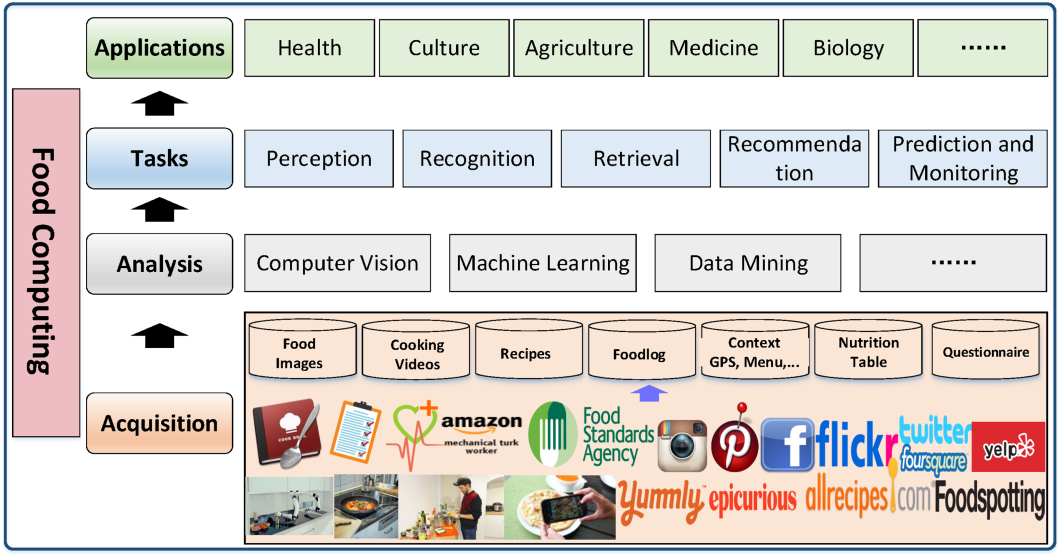
\includegraphics[width=1.0\textwidth]{imagenes/food_computing_1.png}
    \caption{Food Computing}
    \label{fig:food_computing_1}
\end{figure}

En términos generales, las tareas llevadas a cabo dentro del cuadro del Food Computing se caracterizan por partir de un procedimiento de extracción de información, el cual deriva en el desarrollo de herramientas cuyas tareas se pueden englobar en labores de reconocimiento de imágenes, percepción, recomendación, predicción y recuperación de información. De estas tareas destaca especialmente el aprendizaje predictivo, por su papel fundamental en la resolución de problemas en Food Computing~\cite{min2019survey}. Es tal su relevancia que no solo se corresponde con una de las tareas fundamentales abordadas en este ámbito, sino que también cobra protagonismo en las otras mencionadas, bien ocupándose de funcionalidades muy específicas, bien a nivel global, con el fin de dotar de \textit{inteligencia} a la solución (p.ej., capacidad de decisión, identificación de entidades, detección de comportamientos anómalos o previsión de comportamientos futuros que pueda tener un sistema). 

La aplicación de estas tareas no solo afecta a la nutrición sino que también utilizan conocimiento específico de otras áreas para abordar problemas relacionados con la alimentación tales como la medicina, la biología, la gastronomía la agronomía o la cultura. En la Figura \ref{fig:food_computing_1} se muestra un esquema simplificado de todo lo que engloba el concepto de Food Computing~\cite{min2019survey}. 
En ella se aprecia cómo las técnicas predictivas tienen una gran presencia en este campo, ya que además de formar una de las tareas principales, también se encuentran de forma intrínseca en las labores de análisis (Visión por Computador, Aprendizaje Automático y Minería de textos entre otras).

Uno de las mayores desafíos a abordar cuando se trabaja con problemas de Food Computing es la dificultad intrínseca que conlleva el tratamiento de la información. Con ello, no solo nos referimos a la gran cantidad de datos que se generan hoy en día dentro de este contexto, sino también a la dificultad añadida de trabajar con su distinta naturaleza y origen. Abordar un problema de Food Computing suele llevar asociado la necesidad de trabajar de forma simultánea con datos de distintos contextos, como pueden ser la tecnología de alimentos, la nutrición y las redes sociales. %Trabajar de forma conjunta con estos datos es, 
En una primera instancia esto puede resultar inviable, ya que se tratan de fuentes de información muy heterogéneas entre sí, las cuales no se encuentran agregadas y requieren un tratamiento previo que permita poder trabajar con todos los datos de forma simultánea. En esta línea, se pueden utilizar modelos predictivos de lenguaje para identificar elementos equivalentes que se encuentren en dos o más conjuntos de datos, y así poder integrar distintas fuentes y trabajar con ellas como si de una única colección de datos se tratase.

\section{Nuestro problema a resolver}

Tal y como se ha introducido previamente, en el mundo de la alimentación es difícil trabajar con todos los datos requeridos, puesto que las fuentes de información no suelen proporcionarlos de manera directa. Un ejemplo claro son las páginas web de recetas, fuentes de información protagonistas en este ámbito. Normalmente, trabajar con estas recetas desde un punto de vista nutricional requiere de un uso conjunto de sus ingredientes con una base de datos de composición de alimentos para así poder extrapolar su información nutricional. 

Para trabajar de forma conjunta con ambas fuentes de información se requiere un proceso intermedio que haga de intermediario y facilite el tratamiento de datos de distinta naturaleza y origen. Esta idea se refleja en la Figura \ref{fig:heterogeneos_}, donde se puede ver cómo la información alimenticia se nutre de múltiples fuentes de información, dando lugar a un único elemento que se ha denominado en dicha figura como \textit{item food}, que representa al objeto fusionado que se aspira a obtener. Esta dificultad no es específica de Food Computing, sino que se encuentra presente en cualquier área de estudio que combine información de distinto tipo y necesite trabajar con ella de forma conjunta, como puede ser por ejemplo, en el área de medicina al trabajar con datos biomédicos de usuarios y bases de datos de conocimiento o en el área legal, donde fuentes de conocimiento legislativo experto se combinan con sucesos o eventos concretos. 

\begin{figure}[H]
    \centering
    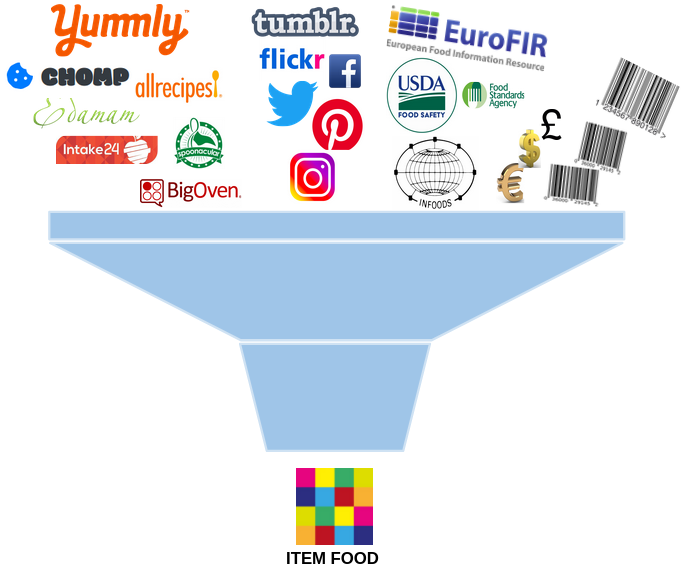
\includegraphics[width=0.8\textwidth]{imagenes/IMAGE.png}
    \caption{Datos heterogéneos en Food Computing}
    \label{fig:heterogeneos_}
\end{figure}

En este trabajo, se desarrolla una herramienta que permite fusionar información heterogénea procedente de diferentes fuentes de datos con el fin de trabajar con ellas simultáneamente. Para ello, se identificarán elementos equivalentes entre las distintas fuentes, para así poder integrarlos y utilizarlos de manera combinada. El problema de identificación de términos equivalentes se puede abordar desde un punto de vista predictivo a partir de varios enfoques. En nuestro caso, lo abordaremos desde la perspectiva del Procesamiento de Lenguaje Natural, utilizando un modelo predictivo de Word Embedding (Word2vec) entrenado con textos de recetas para aprender representaciones de palabras. Con el fin de detectar correspondencias entre los datos, se llevará a cabo un procedimiento de mapeo que utilice dichas representaciones para medir la similitud entre elementos.

%Para ello, se consideran medidas de distancia que tienen en cuenta tanto las características sintácticas del texto, como la información semántica capturada por el modelo. Estas medidas se han estudiado desde las perspectivas clásica y difusa con el objetivo de determinar qué enfoque es el más adecuado para nuestro problema. 
%que nos permita capturar la información semántica de los textos a la hora de obtener su representación. 

Se mostrará su funcionamiento dentro de un sistema que permita su uso para abordar algún problema concreto con los datos ya combinados. En nuestro caso, lo haremos con una aplicación dentro del área de la nutrición, desarrollando un sistema de adaptación de recetas a restricciones alimenticias de usuario, como pueden ser intolerancias a algún alimento, alergias, o incluso restricciones derivadas de dietas como puede ser la vegetariana o la vegana. Este sistema permitirá recomendar, en base a dichas restricciones, posibles variaciones de recetas a través de modificaciones de sus ingredientes. La adaptación de recetas se llevará a cabo gracias al uso previo de la herramienta de fusión de información heterogénea, la cual permitirá combinar recetas de cocina con la información nutricional de sus ingredientes para poder detectar las restricciones alimenticias que deban solventarse.

De las tareas de Food Computing mencionadas anteriormente, con este problema se aborda principalmente un problema de \textbf{Predicción} para la creación de un modelo de lenguaje. Se lleva a cabo el entrenamiento de un modelo predictivo de tratamiento del lenguaje basado en un Word Embedding entrenado sobre un conjunto de recetas que permita identificar términos alimenticios. Por otra parte, también se engloba en otras tareas de Food Computing: sin seguir las estructuras tradicionales y estandarizadas de sistemas basados en recomendación, proporciona opciones de recetas personalizadas a unas preferencias de usuario concretas, resolviendo así un problema en el ámbito de la \textbf{Recomendación} en Food Computing. Problemas de \textbf{Recuperación} e \textbf{Identificación} también se encuentran intrínsecos en este trabajo, puesto que se llevan a cabo tanto la obtención del corpus y fuentes de datos utilizadas para resolver este problema como una tarea de identificación de elementos alimenticios en distintas bases de datos.

\section{Objetivos}\label{sec:objetivos}

Para poder abordar el diseño e implementación de un sistema que permita poner solución al problema descrito en el apartado anterior, se ha marcado como objetivo principal el estudio, diseño e implementación de técnicas predictivas para resolver un problema de Procesamiento de Lenguaje Natural. De este objetivo general se derivan los siguientes objetivos específicos:

\begin{enumerate}
    \item\textit{Identificar los elementos a los que representan los datos que intervienen en el problema}: asignar una representación interna a los datos a través de sus descripciones textuales, con la que poder detectar equivalencias para así realizar la agregación entre las fuentes de datos.

    \item\textit{Fusionar información heterogénea}: desarrollar una herramienta que permita agregar datos de distinta naturaleza y procedencia que necesiten ser tratados de manera conjunta a la hora de abordar algún problema concreto.
    
    \item\textit{Mostrar la eficacia y el alcance de la herramienta desarrollada}: argumentar la utilidad de la herramienta con un problema real y de interés actual: la sustitución de elementos por otros similares mediante el modelo predictivo y las representaciones textuales que genera.
    
\end{enumerate}

\section{Contenido de la memoria en relación a los objetivos}

La memoria se ha redactado en función de los tres grandes pilares en los que se basa este trabajo, los cuales hacen referencia a los tres objetivos específicos detallados en este primer capítulo. En el Capítulo 2 se especifican los requisitos y la planificación por actividades llevada a cabo, las cuales están directamente ligadas a los objetivos. En el Capítulo 3 se exponen los antecedentes que preceden a este trabajo; se profundiza en el concepto de \textit{Food Computing} así como en la revisión bibliográfica de las técnicas de predicción en los problemas abordados en este campo. En el Capítulo 4 se describe de forma general la arquitectura del sistema diseñado para abordar el problema. Se especifican los tres pilares en los que se basa el proyecto como módulos que permiten construir la solución. Estos módulos se relatan de forma detallada en los Capítulos 5, 6 y 7, abarcando el diseño y la implementación llevada a cabo para cada uno de ellos. En el Capítulo 8 se detalla la experimentación y resultados obtenidos en cada uno de los módulos. Por último, en el Capítulo 9, se exponen todas las conclusiones obtenidas a lo largo del trabajo, así como las posibles líneas que se podrían seguir explorando a partir de este trabajo. 

\newpage


\chapter{Planificación y metodología}
\label{ch:Capitulo 2}

\begin{quote}
  Este capítulo presenta los requisitos que debe satisfacer el sistema que se desarrolla en este trabajo, así como su posterior desglose en las actividades a realizar. Por último, se presenta la planificación realizada en base a dichas actividades.
\end{quote}


\section{Especificación de requisitos}

A continuación se enumeran las necesidades que debe satisfacer el sistema desarrollado de acuerdo a los objetivos detallados en la Sección \ref{sec:objetivos}.\\

\textbf{Calidad}
\begin{enumerate}
    \item El modelo de lenguaje debe contener un vocabulario lo suficientemente extenso como para poder trabajar con el lenguaje en el área de estudio escogida.% (prioridad alta).  
    
    \item El modelo de lenguaje tiene que permitir identificar elementos equivalentes entre las fuentes de datos que intervienen en el problema.
    
    \item Los mapeos obtenidos deben ser lo suficientemente fiables como para detectar los ingredientes en recetas y poder acceder a su información nutricional.
    
    \item Las recetas adaptadas deben satisfacer las restricciones que se especifiquen. 
    
    \item La adaptación de recetas debe poder ser interpretable. Para ello, se debe mostrar qué ingredientes no cumplen las restricciones y por tanto deben ser modificados.

    \item Las imágenes de recetas utilizadas en el sistema deben ser lo más representativas posibles.% (prioridad media). % Calidad 
    
    \item La aplicación final debe poseer interfaces gráficas bien formadas que permitan una navegación intuitiva por parte del usuario.% (prioridad medio-alta). % Calidad 
\end{enumerate}

%------------------------------------------------------------------------------------------
\textbf{Escalabilidad}

\begin{enumerate}
    \item El sistema debe ser capaz de controlar grandes volúmenes de datos.% (prioridad alta). % Escalabilidad

    \item El modelo de lenguaje debe poder utilizarse de manera independiente al resto de elementos del sistema. Debe permitir el uso del conocimiento aprendido a otros problemas de Food Computing, así como su reutilización en otros modelos predictivos.
    
    \item La implementación del modelo de lenguaje tiene que posibilitar la opción de realizar, en caso que se requiera, nuevas tareas de entrenamiento con otros corpus distintos del utilizado en este trabajo.% (prioridad media). 
    
    \item El mapeo entre fuentes de datos debe ser independiente de la cantidad de elementos contenidos en cada una de ellas.% (prioridad alta).
    
    \item La adaptación de recetas según restricciones debe ser extensible a nuevas recetas futuras que se añadan al sistema.% (prioridad media).
    
    \item La implementación de la adaptación de recetas debe permitir la incorporación de nuevas restricciones en el futuro.% (prioridad alta).    
    
\end{enumerate}

%------------------------------------------------------------------------------------------
\textbf{Facilidad de mantenimiento}

\begin{enumerate}
    \item El sistema se organizará en distintos módulos, donde cada uno implementará una funcionalidad diferente con el objetivo de que el proceso de modificaciones, pruebas y validación sea más sencillo.% (prioridad baja-medio). % Facilidad de mantenimiento
    
\end{enumerate}

%------------------------------------------------------------------------------------------
\textbf{Facilidad de uso}

\begin{enumerate}
    \item Los usuarios no tienen por qué tener experiencia o conocimientos específicos sobre informática o sobre el proyecto: cualquier usuario debe poder hacer uso de la aplicación final sin dificultad.% (prioridad alta). 
    
    \item La aplicación final debe contar con un pequeño tutorial de la aplicación, para orientar al usuario acerca de cómo funciona el sistema.% (prioridad alta). 
    
    \item Se debe proporcionar un manual de usuario de la aplicación final que permita entender el flujo de datos entre las distintas pantallas implementadas.% (prioridad media). 
    
    \item La aplicación final debe proporcionar mensajes intuitivos para el usuario que le permitan utilizar la aplicación sin dificultad.% (prioridad alta) 

    
\end{enumerate}

%------------------------------------------------------------------------------------------
\textbf{Rendimiento}

\begin{enumerate}
    \item El flujo de datos entre los distintos módulos debe ser el mínimo necesario para optimizar el tiempo de ejecución del sistema.
    
    \item En la aplicación final no habrá excesiva redundancia en cuanto a la información con el objetivo de acelerar las consultas.
    
    \item En la aplicación final solo tendremos acceso a la información de las recetas en cuestión cuando sean seleccionadas.% (prioridad media)

\end{enumerate}

%------------------------------------------------------------------------------------------
\textbf{Robustez}

\begin{enumerate}

    \item El modelo de lenguaje debe proporcionar representaciones para cualquier descripción, controlando las palabras que se queden fuera del vocabulario del modelo.
    
    \item Los mapeos debe contemplar la posibilidad de tratar con descripciones con palabras no contempladas en la representación del modelo de lenguaje.
    

    
\end{enumerate}

%------------------------------------------------------------------------------------------


\section{Actividades}\label{sec:tareas}

Para poder abordar los requisitos detallados en la sección anterior, se ha elaborado la siguiente distribución del trabajo en tres actividades principales, cada una de ellas relativas a los tres grandes bloques que se abarcan en este proyecto. Para el desarrollo de los distintos bloques, se han detallado también las actividades específicas que se llevarán a cabo en cada uno de ellos.
\begin{enumerate}

    \item Diseño y desarrollo de un módulo de Representación del Lenguaje con técnicas predictivas para trabajar con problemas de Procesamiento de Lenguaje Natural en un dominio concreto. % Andrea: ¿Poner DEEP LEARNING o ALGORITMOS PREDICTIVOS?
    
        \begin{enumerate}
            \item Recopilación masiva de datos y creación del conjunto de entrenamiento del modelo con la colección de datos recopilada. 
            
            \item Elaborar técnicas de preprocesamiento de textos para poder trabajar las descripciones textuales de los elementos que se pretenden fusionar.
            
            \item Diseño e implementación de un modelo de Word Embedding y ajuste de hiperparámetros. 
            
            \item Visualización del modelo entrenado con ejemplos concretos para verificar su funcionalidad.
        \end{enumerate}
        
    \item Diseño y desarrollo de un módulo de mapeo de datos que permita fusionar información heterógenea a partir de las descripciones de los elementos a fusionar.
    
        \begin{enumerate}
            \item Diseño de medidas de distancia entre descripciones textuales utilizando su representación textual (previamente preprocesada).

            \item Diseño de medidas de distancia entre descripciones textuales utilizando su representación vectorial obtenida con el modelo de lenguaje.
            
            \item Diseño e implementación de un módulo de mapeo con las medidas de distancia diseñadas.
            
            \item Experimentación y análisis de la eficacia de las medidas de distancia con un problema de mapeo entre dos bases de datos.
            
        \end{enumerate}
            

    \item Experimentación del sistema mediante el desarrollo de una aplicación de adaptación de dietas de usuarios en función de sus restricciones alimenticias.
    
    \begin{enumerate}
        \item Implementar un sistema para aplicar la herramienta de fusión de datos desarrollada.
        
        \item Desarrollar un módulo de consultas adaptadas que permita obtener recetas adecuadas a restricciones.
        
        \item Detectar ingredientes de recetas no sujetos a las restricciones indicadas y subtituirlos por alimentos que sí las satisfagan. 


        \item Implementación de una aplicación móvil para realizar consultas adaptadas sobre las recetas. 


    \end{enumerate}
    
\end{enumerate}

\section{Planificación}

% Planificación en base a las tareas en las que se divide el trabajo. 
La planificación se realizado en función de las actividades definidas en la Sección \ref{sec:tareas}. En la Tabla \ref{tab:actividades} se puede ver la duración asociada a cada una de estas actividades. Tal y como se aprecia en dicha tabla, la planificación se ha estimado de forma semanal. Nótese que se ha establecido un identificador para cada una de las actividades definidas en este proyecto. De esta forma, podemos establecer las dependencias entre las distintas actividades (ver columna \textit{Predecesores} en Tabla \ref{tab:actividades}) para poder generar el diagrama de Gantt (ver Figura \ref{fig:gantt}).

\begin{table}[H]
\centering
\small
\begin{tabular}{cccc}
\textbf{ID} & \textbf{Descripción} & \textbf{Duración (Sem.)} & \textbf{Predecesores} \\ \hline 

A & Actividad 1a & 2 & - \\
B & Actividad 1b & 3 & A \\
C & Actividad 1c & 8 & B\\
D & Actividad 1d & 1 & C \\ \hline

E & Actividad 2a & 4 & B \\
F & Actividad 2b & 4 & C \\
G & Actividad 2c & 2 & E,F \\
H & Actividad 2d & 7 & G \\ \hline

I & Actividad 3a & 2 & G \\
J & Actividad 3b & 2 & I \\
K & Actividad 3c & 2 & J \\
L & Actividad 3d & 18 & K \\ \hline

M & Redacción de la memoria & 27 & - %D,E,G
\end{tabular}
\caption{Actividades llevadas a cabo en el proyecto \label{tab:actividades}}
\end{table}

\begin{figure}[H]
    \centering
\begin{ganttchart}[expand chart=1.0\textwidth,
    canvas/.append style={fill=none, draw=black!5, line width=.75pt},
    hgrid style/.style={draw=black!5, line width=.1pt},
    vgrid={*1{draw=black!5, line width=.75pt}},
    today rule/.style={
      draw=black!14,
      dash pattern=on 3.5pt off 4.5pt,
      line width=1.5pt
    },
    today label font=\small\bfseries,
    title/.style={draw=none, fill=none},
    title label font=\bfseries\footnotesize,
    title label node/.append style={below=7pt},
    include title in canvas=false,
    bar label font=\mdseries\small\color{black!70},
    bar label node/.append style={left=0.1cm},
    bar/.append style={draw=none, fill=blue!300},
    bar incomplete/.append style={fill=barblue},
    bar progress label font=\mdseries\footnotesize\color{black!70},
    group incomplete/.append style={fill=groupblue},
    group left shift=0,
    group right shift=0,
    group height=.1,
    group peaks tip position=0,
    group label node/.append style={left=.1cm},
    group progress label font=\bfseries\small,
    link/.style={-latex, line width=1.5pt, linkred},
    link label font=\scriptsize\bfseries,
    link label node/.append style={below left=-2pt and 0pt},
    y unit chart = 6mm]{1}{44}
  \ganttset{bar height=0.35}
%   \gantttitle[]{Diagrama de Gantt del trabajo}{44}\newline  
    \gantttitle{Sep}{4}
    \gantttitle{Oct}{4}
    \gantttitle{Nov}{4}
    \gantttitle{Dic}{4}
    \gantttitle{Ene}{4}                      % title 3
    \gantttitle{Feb}{4}
    \gantttitle{Mar}{4}
    \gantttitle{Abr}{4}
    \gantttitle{May}{4}
    \gantttitle{Jun}{4}
    \gantttitle{Jul}{4}\\
  \ganttbar[
    % progress=75,
    name=A
  ]{\textbf{Actividad 1a} A}{1}{2} \\
  \ganttbar[
    % progress=67,
    name=B
  ]{\textbf{Actividad 1b} B}{3}{5} \\
  \ganttbar[
    % progress=50,
    name=C
  ]{\textbf{Actividad 1c} C}{7}{14} \\
  \ganttbar[
    % progress=0,
    name=D
  ]{\textbf{Actividad 1d} D}{17}{18} \\[grid]
  
  \ganttbar[name=E]{\textbf{Actividad 2a} E}{6}{9} \\
  \ganttbar[name=F]{\textbf{Actividad 2b} F}{15}{18} \\
  \ganttbar[name=G]{\textbf{Actividad 2c} G}{19}{20} \\
  \ganttbar[name=H]{\textbf{Actividad 2d} H}{22}{28} \\ [grid]
  

  \ganttbar[name=I]{\textbf{Actividad 3a} I}{21}{22} \\
  \ganttbar[name=J]{\textbf{Actividad 3b} J}{23}{24} \\
  \ganttbar[name=K]{\textbf{Actividad 3c} K}{25}{26} \\
   \ganttbar[name=L]{\textbf{Actividad 3d} L}{27}{38} \\
   \ganttbar[name=M]{\textbf{Actividad 4a} M}{15}{43} 
  \ganttlink[link type=f-s]{A}{B}
  \ganttlink[link type=f-s]{B}{C}
  \ganttlink[link type=f-s]{C}{D}
  
  \ganttlink[link type=f-s]{B}{E}
  \ganttlink[link type=f-s]{C}{F}
  \ganttlink{E}{G}
  \ganttlink[link type=f-s]{F}{G}
  \ganttlink[link type=f-s]{G}{H}
  
  \ganttlink[link type=f-s]{G}{I}
  \ganttlink[link type=f-s]{I}{J}
  
  \ganttlink[link type=f-s]{J}{K}
  \ganttlink[link type=f-s]{K}{L}

\end{ganttchart}
\caption{Diagrama de Gantt}
\label{fig:gantt}
\end{figure}

\section{Estimación de costes}


% Costes de ordenador
Para poder estimar los costes de este proyecto debemos distinguir entre los costes de personal y de recursos computacionales utilizados.
Para el cálculo de los costes derivados del personal que colabora en este proyecto, se ha llevado a cabo una estimación por descomposición en actividades medida en \textit{p.m.}{\footnote{p.m. (persona-mes): si un proyecto toma \textit{x} p.m. significa que si se pudieran contratar \textit{x} personas, el proyecto se terminaría en 1 mes o bien, significa que si sólo contratamos a una persona entonces el proyecto se terminaría en \textit{x} meses,}}. En la Tabla \ref{tab:estimacion} se muestra una estimación del esfuerzo que sería necesario para abordar las distintas actividades en las que se divide este proyecto.

\setlength{\tabcolsep}{5pt} 
\begin{table}[H]
\centering
\begin{tabular}{lccccc|c}
\textbf{Actividad} & \textbf{Plan} & \textbf{Análisis} & \textbf{Diseño} & \textbf{Desarrollo} & \textbf{Test
} & \textbf{Total} \\ \hline \hline

\textbf{Actividad 1}  & \textbf{0.4} & \textbf{0.4} & \textbf{1.4} &\textbf{ 1.1} &\textbf{ 0.7 }&\textbf{ 4.0} \\ \hline
Actividad 1a & 0.1 & 0.0 & 0.1 & 0.4 & 0.0 & 0.6 \\
Actividad 1b & 0.1 & 0.1 & 0.5 & 0.1 & 0.2 & 1.0 \\
Actividad 1c & 0.1 & 0.2 & 0.7 & 0.4 & 0.2 & 1.6 \\
Actividad 1d & 0.1 & 0.1 & 0.1 & 0.2 & 0.3 & 0.8  \\ \hline \hline

\textbf{Actividad 2 }& \textbf{0.4} & \textbf{1.2 }& \textbf{0.7} & \textbf{0.35} & \textbf{0.9} & \textbf{3.55}  \\ \hline
Actividad 2a & 0.1 & 0.4 & 0.2 & 0.0 & 0.2 & 0.9 \\
Actividad 2b & 0.1 & 0.5 & 0.2  & 0.0 & 0.2 & 1.0 \\
Actividad 2c & 0.1 & 0.2 & 0.2 & 0.25 & 0.2 & 0.95 \\
Actividad 2d & 0.1 & 0.1 & 0.1 & 0.1 & 0.3 & 0.7 \\ \hline \hline

\textbf{Actividad 3 }& \textbf{0.3} & \textbf{0.35} & \textbf{1.0} & \textbf{0.95} & \textbf{0.75} & \textbf{3.35} \\ \hline
Actividad 3a & 0.1 & 0.1 & 0.1 & 0.1 & 0.1 & 0.5 \\
Actividad 3b & 0.1 & 0.1 & 0.2 & 0.15 & 0.2 & 0.75 \\
Actividad 3c & 0.0 & 0.05 & 0.1 & 0.1 & 0.15 & 0.4 \\
Actividad 3d & 0.1 & 0.1 & 0.6 & 0.6 & 0.3 & 1.7 \\ \hline \hline

\textbf{Total} & \textbf{1.1} & \textbf{1.95} & \textbf{ 3.1} &\textbf{ 2.4} & \textbf{2.35} & \textbf{10.9}
\end{tabular}
\caption{Estimación de costes en p.m. por descomposición de actividades\label{tab:estimacion}}
\end{table}

A estos costes de personal habría que añadirle los asociados a los recursos computacionales necesarios. En este punto hay que considerar la capacidad de procesamiento y de memoria del ordenador para poder entrenar y alojar un modelo predictivo además de una aplicación multiplataforma. En nuestro caso, hemos utilizado un ordenador portátil de gama alta, y el coste asociado a su uso se estima en 700\euro.


\begin{itemize}
    \item \textbf{Costes por recursos computacionales}: 700\euro
    \item \textbf{Costes laborales}: 1600\euro/p.m.
    \item \textbf{Estimación}: 700\euro + 1600\euro/p.m. * 10.9 p.m. = 18140\euro
\end{itemize}

Mediante la estimación por descomposición de actividades el coste del proyecto se estima en 18140\euro.

\chapter{Antecedentes}
\label{ch:Capitulo 3}

\begin{quote}
  Este capítulo presenta los antecedentes que preceden a este trabajo, así como las líneas de investigación y los trabajos previos centrados en tareas predictivas en el campo de Food Computing.
\end{quote}


\section{Food Computing}

Como ya se ha introducido en el Capítulo \ref{ch:introduccion}, el desarrollo de las nuevas tecnologías y el incremento del interés de la población acerca de la alimentación saludable ha contribuido al aumento en la cantidad de datos generados en este campo. 
Este aumento ha dado pie a su tratamiento con algoritmos que puedan procesar grandes cantidades de información con el fin resolver problemas de interés para la población. Aquí tienen especial protagonismo aquellos que son resultado de la interacción entre usuarios en redes sociales o comunidades de usuarios con interés específico en la cocina para predecir valores de sobrepeso y diabetes en la población~\cite{Fried2015,Abbar2015}. Por otro lado, las páginas web y comunidades de usuarios cuyo objetivo específico es compartir recetas (como pueden ser AllRecipes\footnote{\url{www.allrecipes.com}} o Yummly\footnote{\url{www.yummly.com}}), son hoy en día el origen de la mayor parte de colecciones de datos alimenticios en Food Computing~\cite{min2019survey}. En estas páginas, encontramos multitud de recetas con contenido tanto textual, multimedia, como en muchos casos, nutricional. Debido al gran impacto que tienen, múltipes estudios parten de estos datos para la implementación de herramientas o sistemas en Food Computing~\cite{10.3389/fict.2018.00014,10.1007/978-3-319-02432-5_19}.

Sin embargo, si nos fijamos en estas últimas fuentes de datos mencionadas, cada vez es mayor la tendencia hacia recetas con una fuerte componente no saludables. Hoy en día, la concienciación de la población ha dado lugar al desarrollo de movimientos de vida sana basados en la alimentación, los cuales llevan a las personas a interesarse cada vez más por estas recetas. Aquí reside el interés en el desarrollo de herramientas informáticas que puedan adaptar recetas a necesidades de usuarios, ya sea facilitando dietas completas (o bien recetas) adaptadas al usuario, así como con la creación de las llamadas pseudo-recetas, las cuales se centran en generar recetas en base a unas especificaciones dadas, ya sea de forma completa (generación de recetas completas utilizando por ejemplo redes de sabores y grafos de ingredientes con recetas) o parcial (modificando ingredientes concretos dentro de recetas)~\cite{chen2019eating}. En este trabajo se profundiza en esta segunda línea. 

El otro gran foco de información reside en las bases de datos de composición de alimentos, las cuales permiten acceder a la información nutricional de ingredientes, recetas, o incluso platos preparados~\cite{spanishStandariz}, siendo la base de los estudios alimenticios desde el punto de vista de ciencias como la química y la tecnología de alimentos. En este punto destacan bases de datos como la proporcionada por USDA (United States Department of Agriculture)~\cite{gebhardt2008usda}, la cual es una base de datos de referencia a nivel mundial en cuanto a composición nutricional se refiere~\cite{raper2004overview}. También tienen relevancia las bases de datos de composición nutricional de países europeos disponibles en EuroFIR (European Food Information Resource Network)~\cite{church2009eurofir}.
Ya sea de manera individual o conjunta, estos dos grandes focos de información forman el punto de partida de las principales vías de investigación en Food Computing: cocinas internacionales (y el análisis de dietas y recetas derivadas de dichas cocinas) y estudio de composición de alimentos (mayormente orientado a la tecnología de alimentos). Por tanto, las tareas abarcadas en este área tienen como origen uno de estos dos tipos de fuentes de información (o ambos).

\vspace{0.3cm}
A pesar de la gran extensión de tareas que abarca Food Computing, estas se pueden clasificar en cinco grandes grupos en función de los objetivos que persiguen: percepción, reconocimiento de imágenes, recomendación, predicción y recuperación de información, detalladas a lo largo de esta sección.

\subsubsection{Percepción}
La percepción humana acerca de los alimentos influye de forma directa en los hábitos alimenticios. Por ello, esta tarea es ampliamente estudiada en Food Computing desde el punto de vista de la neurociencia y las ciencias cognitivas. Aquí toma importancia el \textit{factor sensorial} de los alimentos donde se incluyen el sabor, la textura o incluso características superficiales del alimento (p.ej., el color o el brillo). La impresión y las sensaciones que provocan los alimentos influyen en la opinión humana de los que los consumen, existiendo una relación entre éstas y los hábitos alimenticios de la gente. En los últimos años han empezado a surgir líneas de investigación que enfocan estos problemas con Aprendizaje Automático y Redes Neuronales~\cite{ofli2017saki}.

\subsubsection{Reconocimiento de imágenes}
El reconocimiento o identificación de elementos del mundo culinario es otro de los problemas más abordado en este ámbito. En esta línea, el reconocimiento de los denominados \textit{item food}, se ha vuelto una tarea esencial en Food Computing. En concreto, el procesamiento de imágenes es sin duda el mayor foco de atracción en este contexto, el cual ya ha sido abordado de múltiples formas: etiquetado de recetas, identificación de ingredientes y grupos alimenticios en grandes bancos de imágenes, etc. En los últimos años, ha aumentado exponencialmente la resolución de estos problemas a partir de técnicas predictivas. Las últimas tendencias residen en combinar la información obtenida a partir del procesamiento de estas imágenes con información de otras fuentes, dando lugar a un conjunto de información de mayor completitud que permita alcanzar mayor precisión en los resultados.

\subsubsection{Recomendación}
Los sistemas de recomendación forman una de las áreas más explotadas en el campo de la alimentación estos últimos años. Conllevan el desafío de información compleja y polifacética, y esto es lo que la diferencia de las tareas de recomendación centradas en otra áreas, donde puedan existir distintos estándares o componentes más objetivas y, por tanto, más sencillas de calcular e interpretar. Principalmente, han abarcado dos vías que merece la pena destacar. Por una parte, la recomendación basada en las preferencias del usuario en cuestión, teniendo en cuenta para ello sus gustos, sus rutinas, así como patrones en cuanto alimentación que a simple vista puedan ser más complicados de detectar. Por otra parte, se le suma a estos sistemas de recomendación la inmersión en el mundo de la nutrición y vida sana, dando lugar a sistemas que persiguen proporcionar asesoramiento dietético personalizado para el usuario, el cual conlleva una fuerte componente saludable. Está muy ligada a las tareas de predicción, sobre todo, para la parte relativa a la recomendación en función de las preferencias del usuario, lo que suele llevar asociado tareas predictivas~\cite{min2019survey}. En los últimos años, se ha producido un auge en el desarrollo de sistemas de recomendación centrados en la generación de dietas personalizadas teniendo como requisito que sean saludables~\cite{Trattner2017}. 


\subsubsection{Predicción}
La gran cantidad de datos que se produce en este área ha dado lugar a que se empleen técnicas predictivas para resolver problemas de Food Computing. Multitud de parámetros, sobre todo relativos a los alimentos, se han estudiado desde el punto de vista de la predicción.  A pesar de los grandes avances que se han hecho en los últimos años, la complejidad intrínseca en los datos, así como las relaciones entre ellos, hacen que realmente este tipo de tareas tenga éxito en entornos muy controlados y restringidos, y para una cantidad concreta de elementos. En escenarios reales, la variedad de casuísticas y factores a considerar es tan grande que, junto con la falta de estandarización, hace inevitable tener que acotar el problema, reduciendo así las probabilidades de éxito que tendría su aplicación en otras fuentes externas. Entre muchas otras, se ha hecho especial hincapié en la evaluación de propiedades de alimentos, seguridad alimentaria y aspectos culturales. 

Por otra parte, tal y como se ha mencionado en los apartados de tareas relativas a Recomendación y Reconocimiento, su aplicación no queda reducida a un campo concreto de Food Computing, sino que se ve aplicada en múltiples ámbitos. En la Sección \ref{sec_pred} se profundiza en los problemas abarcados en literatura que incluyan técnicas predictivas para su resolución.

\subsubsection{Recuperación de información}
Las tareas relativas a la recuperación de datos alimenticios pueden no tener aplicaciones directas, pero sí son de vital importancia para que el resto de tareas que se han detallado anteriormente en esta sección puedan desarrollarse de manera apropiada y proporcionen resultados de calidad: la recopilación de un dataset extenso de imágenes de platos de comida puede no tener un gran impacto en sí mismo, pero la existencia de estos facilita el diseño y desarrollo de técnicas que sí precisen de grandes cantidades de datos, por ejemplo, para entrenar o validar los modelos obtenidos~\cite{marin2019recipe1m+}. Es por ello que un motor de recuperación de información culinaria se hace indispensable para poder trabajar con estas grandes colecciones de datos.


\section{Técnicas predictivas en Food Computing}\label{sec_pred}

\subsection{Aproximaciones generales}

Desde el punto de vista de la predicción en Food Computing se ha estudiado en amplitud patrones intrínsecos en loa alimentos con objetivos muy dispares. En concreto, se ha hecho especial hincapié en la evaluación de propiedades, sobre todo relacionadas con componentes bioactivos y características psicoquímicas de los mismos. En \cite{Correa2018} se recopilan algunos de los estudios llevados a cabo en este ámbito, como la evaluación de las características antioxidantes de los aceites o el determinar la tasa de fermentación de las semillas de cacao en función de medidas de aminoácidos y de cambios de color en los alimentos. Además de estudiar sus propiedades, el análisis y evaluación de los alimentos en el mercado también han tenido un gran protagonismo en las tareas predictivas realizadas en este campo. Se han llevado a cabo estudios  realizados en base a monitorización con tratamientos térmicos, como medio para determinar estados de buena calidad en productos alimenticios. También se pueden consultar en la literatura de Food Computing algunos estudios acerca de la conductividad térmica de productos de panadería, así como de patrones en base al nivel de deshidratación de frutas, estableciendo una relación con la pérdida de agua. Por otra parte, se han realizado estudios que buscan predecir la relación entre la carga de bacterias y la concentración de las mismas en determinados vegetales, concretamente en el tomate y en las hojas de lechuga \cite{Correa2018}. 

Otro campo explotado desde estas técnicas ha sido el de la seguridad alimentaria, donde se han llevado a cabo estudios que buscan determinar el tiempo de caducidad de determinados productos, así como predecir el estado ideal de refrigeración de platos cocinados, o la calidad de los alimentos en función de su conservación en frío. Los problemas de predicción también han cobrado protagonismo en lo que concierne a tareas de clasificación. En \cite{Correa2018} se propone una metodología para clasificar distintos tipos de aceite, vinagre, o incluso de variedades de queso. También se han estudiado clasificadores de grupos alimenticios a partir de parámetros como pueden ser la claridad, el color, el grado de fermentación o incluso la acidez\cite{min2019survey}. 

Por otra parte, las técnicas basadas en el uso de Redes Neuronales también tienen presencia en el mundo culinario, abarcando principalmente tres vías, que se podrían resumir en predicción de parámetros, clasificación y estudios de calidad. Asimismo, las Series Temporales también tienen cabida en este sector, aunque principalmente han tenido presencia desde un punto de vista médico. En \cite{bellaci-biomedical} se hace uso de estas técnicas para interpretar datos procedentes de la monitorización de pacientes con diabetes, intentando evaluar la salida obtenida con una terapia concreta. Otros estudios exitosos se centran en el estudio de los precios u otras características económicas dentro del mundo de la comida \cite{Zou20072913}. En esta área, también entran estudios relativos a la detección de enfermedades en plantas (en vista a la detección de brotes). En \cite{towards-food-security-ia} estudian la detección de la enfermedad \textit{Blast} en la hoja del arroz a partir de técnicas predictivas en procesamiento de imágenes.

Si nos centramos en el análisis a nivel de receta y no de alimento, es posible aprovechar la detección de ingredientes y los métodos de predicción de la cocina para comparar los alimentos en función de sus componentes~\cite{Singh2015CSE2A}. De manera similar, se puede identificar el país de origen de la receta utilizando términos extraídos del texto~\cite{Min2018YouAreWhat}. Asimismo, otro campo de estudio en el que se han centrado diferentes problemas de predicción ha sido en los aspectos multiculturales relativos al mundo culinario, analizando datos de distintas zonas geográficas a nivel mundial~\cite{Sajadmanesh2019}. La relación entre propiedades de ingredientes, influencia de la región y hábitos alimenticios han sido objeto de estudio en Food Computing durante los últimos años~\cite{Min2018} en lo referente a enfermedades relacionadas con la alimentación. También se han analizado patrones de combinación de ingredientes en distintas regiones~\cite{Bossard2014} para la búsqueda de equivalencias de cocina regional de unas zonas geográficas a otras totalmente dispares~\cite{10.3389/fict.2018.00014}. Sin embargo, los trabajos en este área se han visto limitados por la ausencia de herramientas que permitan gestionar de forma conjunta bases de datos de composición nutricional de distinta procedencia geográfica. Este problema ha sido expuesto en múltiples trabajos~\cite{spanishStandariz}, dando lugar a una necesidad de herramientas de fusión de información de distintas fuentes de datos. La falta de estandarización en los datos y la ausencia de una base de datos estandarizada impide realizar estudios más allá de entornos específicos muy controlados.

\subsection{Modelos predictivos del lenguaje}

Si nos centramos en el uso de técnicas predictivas en Food Computing para el procesamiento de información textual, no han tenido tanto recorrido en comparación con las tareas predictivas mencionadas en la sección anterior. Uno de los trabajos más destacados es \textit{Food2Vec}, donde se utiliza un modelo de Word Embedding entrenado con las listas de ingredientes incluidos en las recetas~\cite{food2vec}. Otro modelo de Word Embedding también entrenado en el ámbito culinario es Recipe2Vec~\cite{recipe2vec}, que aunque codifica todo el texto, se centra en la comparación y recuperación de recetas (además, de no ser código abierto). Sí que se han expuesto las ventajas de un modelo de fusión de información heterogénea en Food Computing, en el que se integren imágenes, textos e información nutricional procedente de recetas~\cite{8099810}. Sin embargo, este último modelo está enfocado a tareas de reconocimiento de imágenes, y los datos textuales que contienen son minoría y no bastan por sí solos para desarrollar un modelo de Procesamiento de Lenguaje Natural.

Además, debemos tener en cuenta que los textos, sobre todo procedentes de recetas suelen incluir marcas de alimentos, ya que, una de las propiedades más características del lenguaje alimenticio es la utilización de manera indistinta de marcas y los nombres de alimentos representados por dichas marcas. En este tipo de textos, a menudo encontraremos marcas sustituyendo a los propios ingredientes. Además, la información de estos productos comerciales también aparece en las bases de datos, por la propia flexibilidad que tienen a la hora de almacenar su información. En consecuencia, nuestro modelo de lenguaje debe permitir lidiar con este tipo de términos. En esta línea, destacamos los trabajos de~\cite{10.1093/jamiaopen/ooz007}, en los que, con un modelo de Word Embedding identificaron, entre otros, nombres de marcas pertenecientes a suplementos dietéticos. Asimismo, se han utilizado modelos de Word Embedding para abordar problemas de evaluación de la calidad de menús de restaurantes, utilizando funciones de puntuación sobre las representaciones vectoriales de platos en los menús de dichos establecimientos~\cite{chao2016dish}.

Más allá de la aplicación de modelos de Word Embedding a recetas y cocinas del mundo, el uso de estos modelos también se ha empleado para detectar similitud a nivel de alimento. Como trabajo destacado en este contexto, se han utilizado representaciones obtenidas con modelos de Word Embedding para enriquecer la red de sabores entre los distintos ingredientes involucrados en recetas, y así poder crear recetas sustitutas en función de factores sensoriales \cite{Sauer2017CookingUF}. En este trabajo, se parte de la hipótesis de que los ingredientes se pueden representar en un espacio de sabores~\cite{ahn2011flavor}, y que a partir de esas representaciones se puede pasar de unos grafos receta-ingredientes a otros, teniendo en cuenta dicha información cognitiva.

Desde una perspectiva más amplia, otros trabajos de investigación estudiaron la relación entre los ingredientes y los métodos de cocción a partir de las descripciones de los datos de los alimentos y redes de sabores. Este último problema ha sido ampliamente abordado en la literatura, sobre todo mediante la aplicación de técnicas personalizadas de procesamiento estadístico de lenguaje natural \cite{Takahashi2012,Chen2017,chang2018recipescape}.

\subsection{Identificación de términos alimenticios textuales}

El problema de mapear términos entre dos fuentes de datos dadas (en nuestro caso, alimenticias) se puede ver como un problema de identificación de términos equivalentes entre dichas fuentes de datos. En las secciones anteriores ya se ha introducido la necesidad de fusionar fuentes de datos de composición nutricional de distinta procedencia. Esta dificultad también ha sido ratificada por otros estudios llevados a cabo sobre estas fuentes de información, los cuales confirman la necesidad de utilizar herramientas informáticas que permitan automatizar la unificación de bases de datos de composición nutricional de alimentos~\cite{barabasi2019unmapped}.

Estas bases de datos se caracterizan por una alta complejidad, nivel de detalle, y periodicidad con la que nueva información de este campo se actualiza (o directamente se genera información nueva), formando el llamado \textit{agujero negro} de la nutrición~\cite{barabasi2019unmapped}. Por ello, el esfuerzo en fusionar fuentes de datos de esta naturaleza se ha centrado fundamentalmente en el mapeo entre atributos de distintas bases de datos nutricionales, con el objetivo de unificar las características nutricionales de los alimentos~\cite{ispirovaG} y así llevar a cabo comparativas a nivel nutricional entre ellas, en este caso, por medio de una ontología.

El uso de ontologías para poder trabajar de forma simultánea con más de una base de datos de composición nutricional ha tenido un largo recorrido~\cite{snae2008foods,dooley2018foodon,6511683}. Un ejemplo de ello es EuroFIR\footnote{\url{http://www.eurofir.org/}} (European Food Information Resource Network), cuya ontología permite, a través de su buscador \textit{FoodExplorer}, mostrar en un formato armonizado el contenido e información nutricional de múltiples alimentos procedentes de bases de datos europeas~\cite{sheehan2008european}. En este ámbito tienen especial protagonismo las ontologías \textit{LanguaL}~\cite{ireland2010langual} y \textit{FoodEx2}~\cite{european2015food}, por su completitud así como por el reconocimiento de los organismos oficiales que las mantienen: US Food and Drug Administration (FDA)\footnote{\url{https://www.fda.gov/}} en el caso de \textit{LanguaL} y European Food Safety Authority (EFSA)\footnote{\url{https://www.efsa.europa.eu/}} en el caso de \textit{FoodEx2}. Sin embargo, la falta de estandarización y los niveles de detalle superficiales alcanzados por dichas ontologías (representan agrupaciones por grupos y subgrupos alimenticios), impiden poder ser utilizadas  para la unificación e identificación a nivel de alimento. Esto hace que las herramientas disponibles de mapeo a nivel de ontología resulten insuficientes para mapear alimentos muy concretos en estas bases de datos~\cite{li2019multi}. 

Desde un punto de vista de tratamiento de información textual, en Food Computing destacan dos vías principales para abordar esta dificultad: el uso de expresiones regulares para extraer información de los alimentos~\cite{chao2016dish}, y utilizar métricas para calcular la distancia entre palabras o textos cortos a partir de modelos de Word Embedding~\cite{Farouk2019MeasuringSS, Kenter2015}, dado el buen funcionamiento que ha tenido a la hora de detectar términos en fuentes de datos externas~\cite{10.1093/jamiaopen/ooz007}. En este contexto, las técnicas de similitud que involucran Lógica Difusa pueden aplicarse para obtener los mapeos entre dos fuentes de datos dadas~\cite{wang2011fast}. Estas técnicas ya han sido probadas anteriormente en el campo de Food Computing para mapear datos alimenticios procedentes de cuestionarios de frecuencia de consumo de alimentos~\cite{10.3389/fnut.2018.00082}.

Más allá de medidas de similitud tradicionales como pueden ser la medida de \textit{Jaccard} o la similitud \textit{Coseno}~\cite{sternitzke2009similarity}, a la hora de detectar equivalencias entre descripciones textuales cortas y modelos de Word Embedding, es destacable mencionar la medida de distancia \textit{Word's Mover}, la cual ha demostrado ser especialmente adecuada para identificar equivalencias a partir de los vectores de documentos cortos obtenidos con Word2Vec~\cite{wmd1,wmd2}.


\chapter{Arquitectura del sistema}
\label{ch:Capitulo 4}

\begin{quote}
  Este capítulo recoge la descripción de la arquitectura del sistema que se ha desarrollado en este trabajo.
\end{quote}

\section{Descripción del sistema}

Como hemos introducido previamente, en este trabajo se va a desarrollar una herramienta que permita trabajar de forma simultánea con datos heterogéneos de distinta procedencia, que posteriormente puedan ser utilizados de forma conjunta en alguna aplicación o problema concreto: en nuestro caso, Food Computing.

\begin{figure}[H]
    \centering
    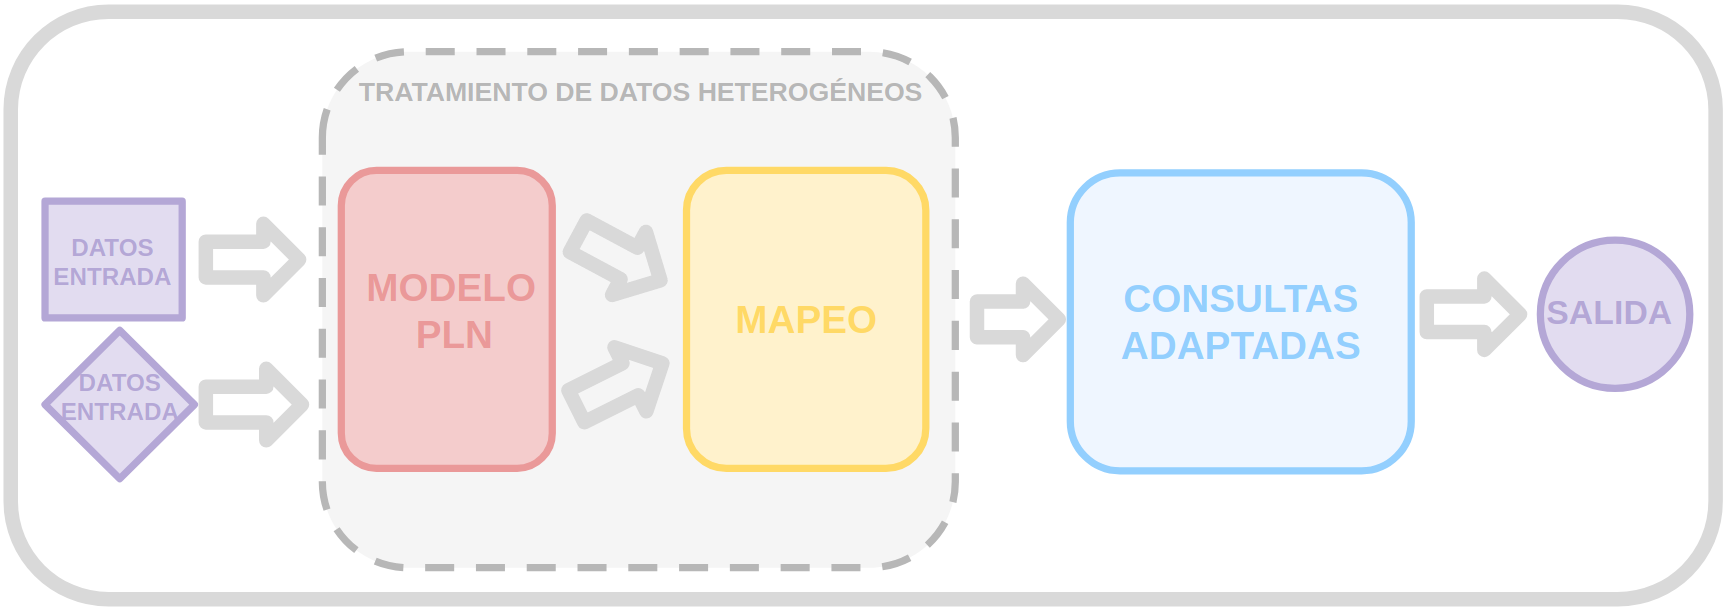
\includegraphics[width=1.0\textwidth]{imagenes/arquitectura/arquitectura-global.png}
    \caption{Arquitectura del sistema}
    \label{fig:arq_1}
\end{figure}

Desde un punto de vista computacional, la resolución de un problema de esta naturaleza se puede modelar como un sistema que funciona en dos fases: una primera fase que se encarga de fusionar los datos de entrada y devolverlos en una estructura que permita poder trabajar con ellos como un todo, y una segunda fase la cual utiliza dicha información fusionada, ya correctamente preprocesada, en el desarrollo de una aplicación que resuelva un problema concreto. Esta idea se puede ver reflejada en la Figura \ref{fig:arq_1}, la cual describe de forma simplificada nuestra propuesta de arquitectura general. En dicha figura se puede observar cómo, a partir de unos datos de entrada heterogéneos entre sí, éstos pasan por un procedimiento que permite trabajar con ellos de forma conjunta (ilustrado en la figura como \textit{Tratamiento de datos heterogéneos}) y poder ser utilizados para llevar a cabo consultas adaptadas a la información una vez fusionada (también apreciable en dicha figura).

\section{Módulos del sistema}

Tal y como se puede apreciar en el esquema de la arquitectura del sistema (ver Figura \ref{fig:arq_1}), las distintas tareas que se llevan a cabo se pueden organizar en módulos independientes, cada uno de ellos ocupándose de una tarea específica que permita cumplir con todos los requisitos del sistema. En dicha figura se pueden apreciar dos primeros módulos, \textit{Modelo de Procesamiento de Lenguaje Natural (PLN)} y \textit{Mapeo}, los cuales se utilizan para el tratamiento con los datos de entrada heterogéneos. Un último módulo denominado \textit{Consultas Adaptadas}, engloba la funcionalidad de un motor de consultas sobre los datos de las distintas fuentes una vez que ya están fusionados.%, representando un único conjunto agregado.

Cada uno de estos módulos es independiente de los demás, y se encarga de una labor específica necesaria para el funcionamiento global del sistema. La funcionalidad de cada uno de ellos, así como su papel en el sistema, se detalla a continuación.

\subsection{Módulo de Procesamiento de Lenguaje Natural}

Este módulo hace referencia al modelo de Procesamiento de Lenguaje Natural (PLN) que se ha implementado para el tratamiento de información textual en este trabajo. Permite obtener una representación de las descripciones textuales de los distintos datos que se introducen como entrada al sistema (ver objetos \textit{Datos entrada} en la Figura \ref{fig:arq_1}). En este punto, se debe tener en cuenta que no hay restricciones previas sobre los datos de entrada más allá de que deban tener descripciones textuales del mismo ámbito para poder llevar a cabo la fusión entre ellos. Por ejemplo, combinar una receta con una base de datos de alimentos a través de las descripciones textuales de los ingredientes de la receta y las de los alimentos de la base de datos de composición nutricional.

Los datos de entrada son procesados en este módulo, para así obtener la representación en el modelo de lenguaje de la descripción textual de cada uno de los datos introducidos. Estos datos pueden ser datos individuales (p.ej., una receta), o un conjunto de ellos (p.ej., colecciones de recetas o bases de datos de alimentos). El componente principal de este módulo, y por el cual se obtienen las representaciones textuales que utiliza el sistema, es un modelo de procesamiento de lenguaje formado por un Word Embedding entrenado en el dominio específico del problema que se pretende resolver. 

En el Capítulo \ref{ch:Capitulo 5} se describe de manera detallada el desarrollo e implementación del modelo de lenguaje. Finalmente, como salida de este módulo, se devuelven las representaciones de las descripciones textuales de los datos que se han proporcionada como entrada al sistema. Las representaciones que se obtienen como salida de este módulo son con las que se trabajará en los módulos restantes que engloban el funcionamiento del sistema. En la Figura \ref{fig:arq_modelo_nlp} se puede ver en mayor detalle el contenido de este módulo. En ella se aprecia el modelo de lenguaje basado en Word Embedding.

\begin{figure}[H]
    \centering
    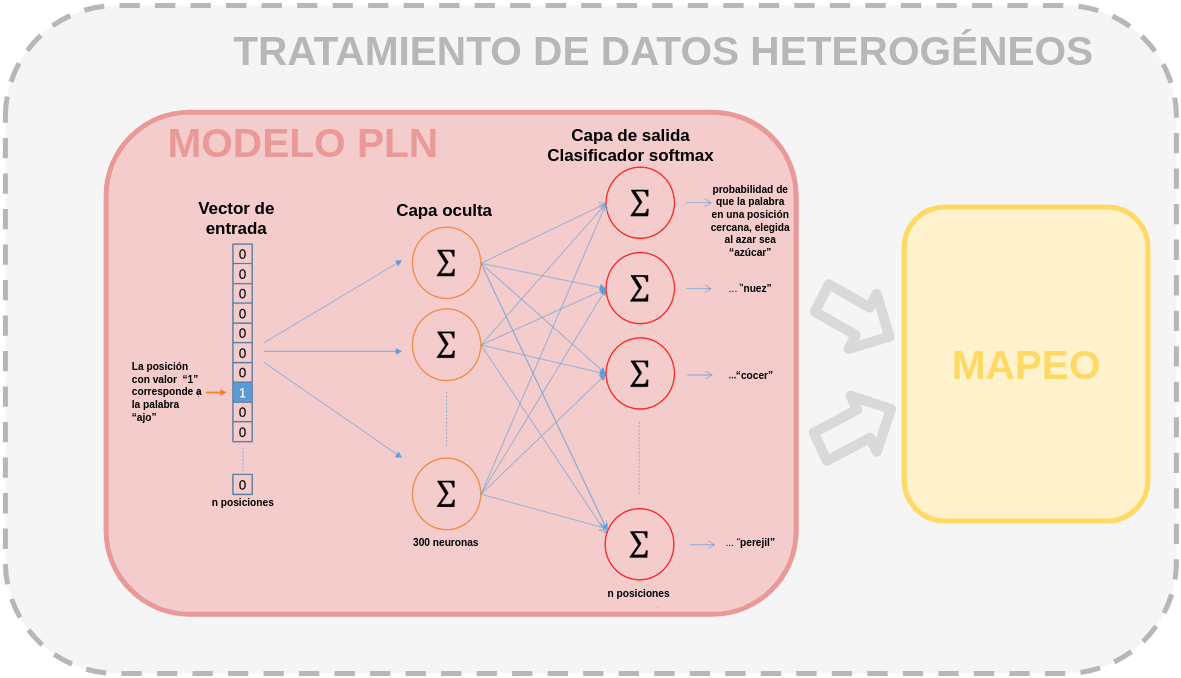
\includegraphics[width=1.0\textwidth]{imagenes/arquitectura/wembedding.png}
    \caption{Arquitectura del sistema: módulo de NLP}
    \label{fig:arq_modelo_nlp}
\end{figure}

\subsection{Módulo de Mapeo}

Este módulo se encarga de identificar las posibles equivalencias entre los datos de entrada, los cuales, como ya se ha mencionado anteriormente, son de naturaleza heterogénea y distinta procedencia. Para ello, se encarga de obtener la mejor correspondencia posible entre los datos proporcionados como entrada al sistema. Este cálculo se realiza en dos pasos:

\begin{enumerate}
    \item En primer lugar se calcula la similitud entre las descripciones textuales de los datos heterogéneos que se han proporcionado. Para ello, se calcula la distancia entre las representaciones que devuelve el módulo de procesamiento del lenguaje de los datos de entrada que se quieren fusionar. Por ejemplo, supongamos que queremos conocer los valores nutricionales de un alimento concreto, y para ello queremos mapear dicho alimento a una base de datos de composición nutricional. En este primer paso, se calcularía la similitud entre el alimento en cuestión y cada uno de los alimentos que se encuentran en la base de datos (los cuales son candidatos a ser el equivalente de dicho alimento en esa base de datos).
    
    \item En segundo y último lugar, se obtiene, de entre todos los posibles candidatos, aquella correspondencia con la que se obtenga la mayor similitud. Volviendo al ejemplo del punto anterior, en este segundo paso nos quedaríamos aquel elemento de la base de datos de composición nutricional cuya similitud con el alimento a fusionar sea máxima.

\end{enumerate}

El funcionamiento que se ha detallado en los dos puntos anteriores se puede ver en la Figura \ref{fig:arq_mapping}, la cual muestra de forma esquematizada las distintas tareas que se abordan en este módulo. Como se puede apreciar en dicha figura, a partir de las representaciones del módulo de procesamiento del lenguaje se establecen correspondencias entre los datos de entrada utilizando el módulo de Mapeo, los cuales permiten trabajar de forma conjunta con los distintos datos que se introducen al sistema.

\begin{figure}[H]
    \centering
    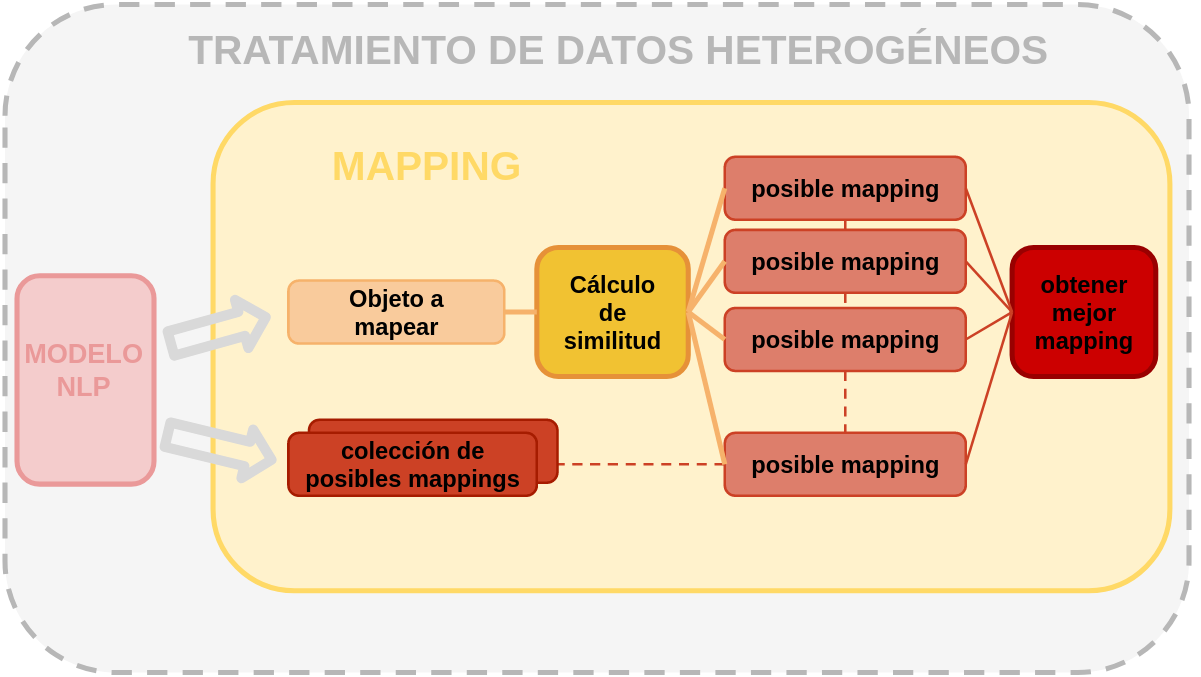
\includegraphics[width=1.0\textwidth]{imagenes/arquitectura/mapping.png}
    \caption{Arquitectura del sistema: módulo de Mapping}
    \label{fig:arq_mapping}
\end{figure}

Debido a la labor general que abarcan tanto este módulo como el de procesamiento de lenguaje, su funcionalidad se puede ver de forma conjunta a más alto nivel, como una única tarea de combinación de información heterogénea llevada a cabo por dos módulos internos independientes. Esta tarea se encarga de establecer las relaciones necesarias entre los datos de entrada para poder trabajar con ellos de forma agregada y así un tercer módulo (en nuestro caso, un módulo de consultas) pueda utilizar dichos datos de forma conjunta. En el Capítulo \ref{ch:Capitulo 6}, se detalla el comportamiento de este módulo.

\subsection{Módulo de Consultas Adaptadas}
A diferencia de los módulos anteriores, los cuales tienen una funcionalidad orientada al tratamiento de las fuentes de datos heterogéneas, la de este último se basa en facilitar la realización de operaciones de consulta que requieran el uso de dichas fuentes de datos de forma simultánea. En otras palabras, a través de este módulo se facilitan los datos, previamente agregados, que resuelvan los requisitos necesarios para el problema en cuestión que se quiera resolver. Estos requisitos dependerán de la tarea específica para la que se quieran utilizar los datos, la cual es independiente tanto de la arquitectura del sistema como del área de aplicación.

\begin{figure}[H]
    \centering
    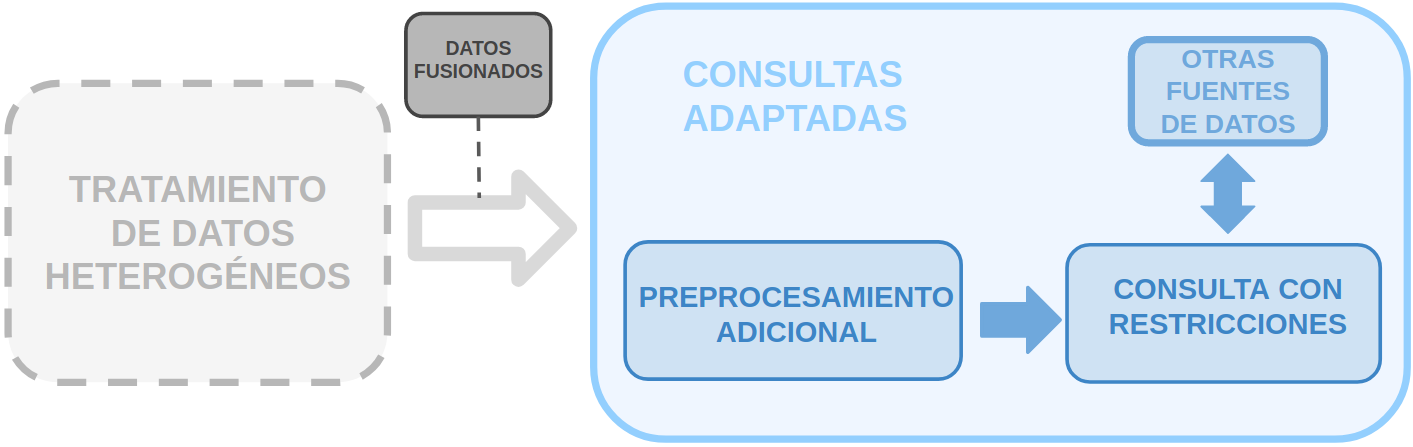
\includegraphics[width=1.0\textwidth]{imagenes/arquitectura/modulo-consulta.png}
    \caption{Arquitectura del sistema: módulo de Consultas Adaptadas}
    \label{fig:arq_application}
\end{figure}

En la Figura \ref{fig:arq_application} se muestra de manera esquematizada la funcionalidad que se implementa en el interior de este módulo. En ella se aprecia cómo se permite obtener la información ya fusionada de manera homogénea por medio de consultas específicas. Estas consultas dependen completamente del problema que se pretende resolver y tal y como se puede ver en dicha figura, aquí pueden incluirse otras bases de datos o algunas tareas adicionales de preprocesamiento para adecuar los datos al uso o tipo de consulta específica llevar a cabo. Este módulo representa el objetivo último del sistema que se ha implementado, y se corresponde con la propia salida del mismo (ver objeto \textit{Salida} en Figura \ref{fig:arq_1}). Su funcionamiento se describe de forma detallada en el Capítulo \ref{ch:Consultas_Adaptadas}.

\section{Sistema para adaptación de dietas en Food Computing}

En este trabajo, se ha implementado una aplicación simple que permita testear el comportamiento y alcance de la herramienta de fusión de datos heterogéneos que se ha desarrollado, probando su funcionamiento en un sistema real como el descrito en los apartados anteriores. Para ello, se ha abordado un problema de gran relevancia en el mundo de la nutrición y el asesoramiento dietético, el cual consiste en aplicar restricciones alimenticias a recetas, adecuando para ello sus ingredientes por otros más idóneos que sí cumplan con dichas restricciones: dada una receta (y sus ingredientes) y una restricción alimenticia concreta, se adaptarán sus ingredientes para que la receta satisfaga las especificaciones proporcionadas. Por ejemplo, una receta con carne podría ser convertida en una receta vegetariana, modificando los ingredientes pertinentes por otros que sí cumplan las restricciones indicadas.

Este sistema se ha implementado como núcleo de una aplicación móvil que gestiona una colección de recetas, permitiendo adaptarlas a una restricción alimenticia concreta seleccionada por el usuario. Para poder abordar esta tarea, se hace uso de la lista de ingredientes correspondiente a la receta en cuestión y de una base de datos de composición de alimentos. Estos datos, de naturaleza claramente heterogénea, necesitan fusionarse para poder conocer las características nutricionales de la receta, y así poder aplicar las restricciones pertinentes. Por ello, se agregan estos datos por medio de la herramienta de fusión de datos heterogéneos, mapeando los ingredientes de la receta con la base de datos de composición nutricional de alimentos de forma que podamos realizar las sustituciones con un respaldo nutricional. Esta secuencia de tareas puede verse en la Figura \ref{fig:arq_application_food_comp}, donde se muestra la arquitectura global del sistema descrito anteriormente, pero ya aplicada al problema en cuestión.

\begin{figure}[H]
    \centering
    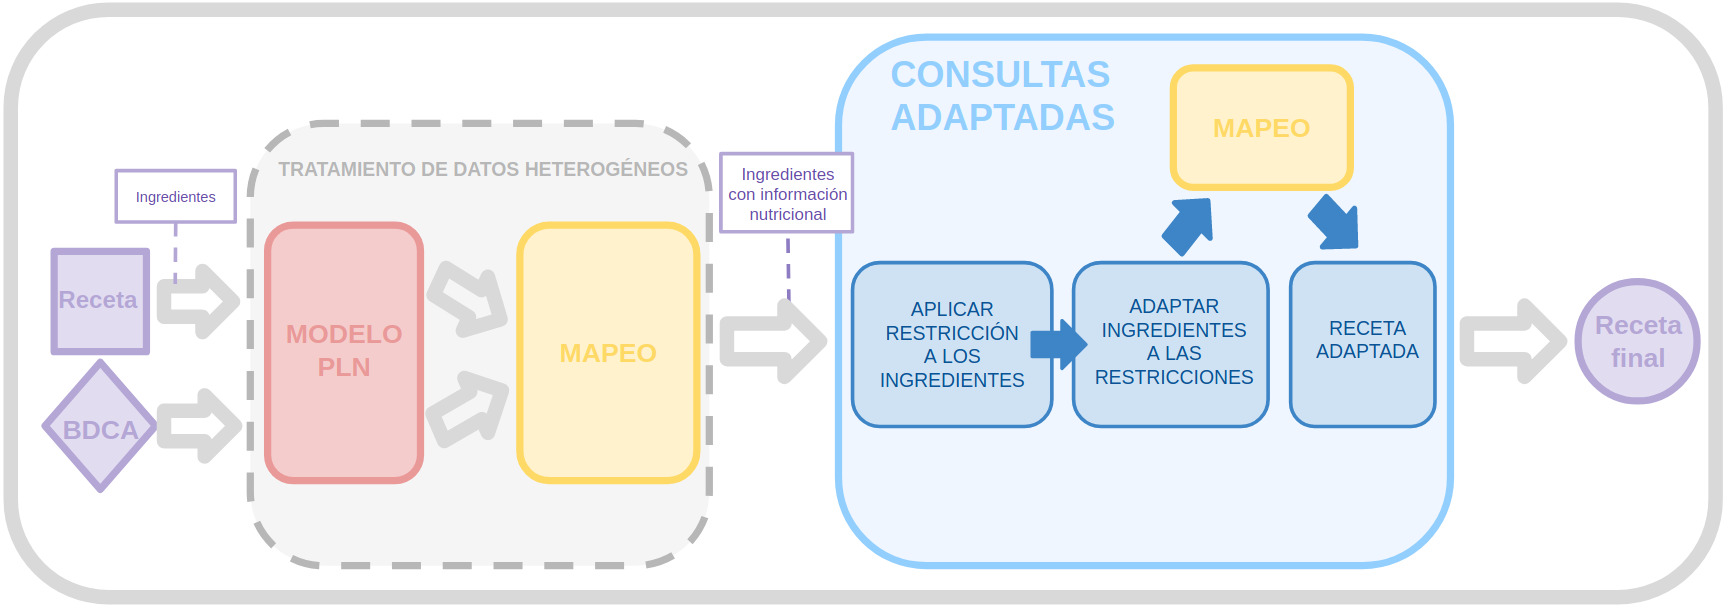
\includegraphics[width=1.0\textwidth]{imagenes/arquitectura/arquitectura-fcomputing.png}
    \caption{Arquitectura del sistema aplicada al problema de adaptación de dietas en Food Computing}
    \label{fig:arq_application_food_comp}
\end{figure}



\chapter{Word Embedding}
\label{ch:Capitulo 5}

\begin{quote}
  Este capítulo introduce el concepto de Word Embedding y describe de forma detallada el modelo desarrollado para este proyecto. 
\end{quote}

% PASADO A LA SECCIÓN DE REVISIÓN BIBLIOGRÁFICA
\section{Introducción a los Word Embeddings}
La comprensión del lenguaje natural a partir de datos textuales es una de las áreas más estudiadas dentro del ámbito de la Inteligencia Artificial. Esto se debe a la necesidad de una forma adecuada para la representación de información textual de manera que ésta pueda ser tratada de forma automática. En la literatura, se han abordado técnicas para resolver este problema bajo distintas perspectivas, las cuales se centran en obtener una representación de palabras o un conjunto de ellas (generalmente frases o párrafos), que nos permitan trabajar con la información que contienen. La forma más sencilla de representar información textual como vector es mediante \textit{one-hot embedding}, donde el mapeo de los datos textuales se realiza con un vector donde cada casilla se asocia al índice de cada palabra y contiene el número de veces que aparece dicha palabra en el texto. Sin embargo, esta representación resulta poco escalable y no funciona bien cuando se trabaja con vocabularios de gran tamaño, ni tampoco tiene en cuenta las relaciones que existen entre una palabra y las que le rodean (lo que resulta indispensable al trabajar con información textual). Este último problema es el que recogen las técnicas basadas en \textit{n-gramas}~\cite{jones2007representing}, las cuales intentan tener en cuenta, no sólo una palabra, sino también aquellas que se encuentran cercanas en el texto con el objetivo de modelar la información de manera más realista. Esta técnica no sólo ha sido aplicada a nivel de palabra, sino que también se han aplicado técnicas basadas en n-gramas a otros niveles, como puede ser al de frase o de carácter~\cite{wieting2016charagram}. Usar n-gramas conlleva la dificultad de determinar qué cantidad de información debe de ser la que se tenga en cuenta para una palabra en cuestión, ya que es difícil determinar (y sobretodo, generalizar) el tamaño de la ventana que se considera a cada lado del elemento a representar. Aun así, en las tareas que involucran Procesamiento de Lenguaje Natural, existen otras dificultades añadidas como pueden ser la ambigüedad del lenguaje, el tratamiento de anáforas o la posibilidad de trabajar con palabras que no se hayan contemplado a la hora de diseñar el modelo del lenguaje en cuestión~\cite{li2018word,anaphora}. Estos problemas han llevado al desarrollo de herramientas más sofisticadas como pueden ser los modelos con métodos basados en Modelo de Espacio Vectorial (VSM) o Asignación Latente de Dirichlet (LDA)~\cite{almeida2019word}. 

El concepto de Word Embedding se introduce con los Modelos de Lenguaje basados en Redes Neuronales (Neural Networks Language Model) basándose en la idea de que es más probable que dos palabras sean similares si se usan en contextos parecidos. La motivación detrás de esta idea reside en que dos palabras con un significado similar deben usarse de forma parecida, y por tanto, su representación debe de ser parecida también. Este tipo de modelos se caracterizan por ser modelos no supervisados, y algunos de las representaciones más conocidas son las unidades LSTM (Long-Short Term Memory), \textit{Redes Neuronales Recurrentes} (RNN) o \textit{Word2Vector}~\cite{li2018word}. El éxito de estos modelos se debe a los buenos resultados que se han obtenido al aplicarlos en problemas que requieran trabajar con información textual. Como consecuencia de ello, se utilizan en multitud de aplicaciones de diferentes campos de estudio y se ha destacado su eficacia respecto a otros métodos a la hora de trabajar con textos~\cite{indefense}. En nuestro caso, el objetivo es definir una representación que nos permita codificar alimentos procedentes de textos de recetas, para así identificar ingredientes y a su vez permitirnos detectar alimentos equivalentes (o incluso de uso equivalente). Este objetivo lo podemos lograr con modelos de Word Embedding puesto que tienen en cuenta el contexto que acompaña a las apariciones de cada palabra en el conjunto de entrenamiento de forma que se mantenga su significado en la codificación, a partir de cuándo, cómo y con qué otras palabras suele aparecer.
%El trabajar con las representaciones que se obtienen por medio de modelos de Word Embedding (las llamadas \textit{representaciones distribuidas}), nos permiten trabajar con codificaciones de palabras que tienen en cuenta la semántica a la hora de representar dicha palabra. Para ello, tienen en cuenta el contexto que acompaña a las apariciones de cada palabra en el conjunto de entrenamiento, de forma que se pueda mantener su significado en la codificación, a partir de cuándo, cómo y con qué otras palabras suele aparecer. 

Esta importancia del contexto a la hora de obtener la codificación de los datos textuales nos permitirá trabajar con los ingredientes de las recetas de manera más precisa, ya que, muchos de estos ingredientes serán similares (o su uso será parecido), o incluso se caracterizarán por poder nombrarse de más de una forma distinta. Como ejemplo de ello tenemos numerosos alimentos para los que se emplean más de un nombre de manera indistinta: sepia y choco, judías y habichuelas, pero y manzana, o incluso galleta y cookie. Además, por las características del lenguaje culinario, hay que tener en cuenta que las diferencias culturales y las marcas de alimentación se suelen ver involucradas con frecuencia en las recetas de cocina. Muchas veces se utiliza la marca del alimento en sustitución del propio alimento (p.ej., \textit{Danone} y yogur, pan \textit{Bimbo} y pan de molde), y otras veces, dependiendo del origen geográfico de la receta, un mismo alimento puede ser referido de distintas formas (p.ej., boniato y batata, melocotón y durazno, etc). El utilizar representaciones que sean capaces de tener en cuenta esta semántica (como es el caso de los modelos de Word Embedding) nos permitirá trabajar de una forma más adecuada con estos problemas y solventar dificultades procedentes del lenguaje como pueden ser las diferencias culturales mencionadas anteriormente, así como las asunciones de conocimiento que se hacen al hablar en términos de recetas y cocina en general. 
 
\section[Word embeddings generales vs específicos]{Word embeddings generales vs específicos en Food Computing}

Hoy en día, existen modelos de Word Embedding de carácter general ya entrenados sobre grandes cantidades de datos textuales procedentes de grandes bases de datos de documentos. Este es el caso, por ejemplo, del modelo Word2vec entrenado por Google\footnote{\url{https://code.google.com/archive/p/word2vec/}}, el cual incluye representaciones vectoriales de palabras para un vocabulario de 3 millones de palabras y frases entrenado a partir de 100 billones de palabras procedentes de un dataset de Google News. Estos modelos permiten abordar de manera eficaz con problemas de Procesamiento de Lenguaje Natural de manera superficial y sin profundizar en campos de conocimiento muy específicos. 

% mas modelos preentrenados aqui https://radimrehurek.com/gensim/auto_examples/howtos/run_downloader_api.html 

Sin embargo, en nuestro caso, al estar trabajando con un dominio tan específico como es el de la nutrición, surge la necesidad de utilizar modelos entrenados sobre dicho dominio concreto. Esto se debe principalmente a la gran cantidad de vocabulario especializado que es difícil de encontrar en un modelo de carácter general, y que limitaría la potencia de éste al no ser capaz de representar las descripciones alimenticias de manera correcta. A la hora de tratar con las descripciones textuales de los alimentos como si se tratasen de documentos cortos, cada una de las palabras pertenecientes al documento es representada usando el modelo de Word Embedding entrenado. Dado que el vocabulario del modelo no engloba todas las palabras de ese lenguaje, muchas de ellas no podrán representarse con este modelo. Estas palabras, denominadas \textit{out-of-vocabulary} (OOV)~\cite{8751687}, suponen un reto en las tareas de Procesamiento de Lenguaje Natural, y existen en la literatura múltiples formas de abordar este problema~\cite{camacho2018word}. Cuando una de estas palabras no tiene representación en el modelo, es omitida (o en algunos casos reemplazada), introduciendo ambigüedad en la representación final de dicho documento. 

En nuestro caso, donde gran parte del vocabulario referente a los alimentos es raramente usado fuera del contexto culinario o nutricional, el uso de un modelo de carácter general intensificaría el problema previamente comentado, dando lugar a representaciones muy precarias. Para ilustrar este problema, pongamos como ejemplo que queremos modelar la descripción alimenticia ``\textit{Tartaletas de escalibada con anchoas}". Teniendo en cuenta el tratamiento de las palabras OOV previamente comentado, supongamos que el modelo no capaz de detectar la palabra \textit{Tartaleta}, y por tanto ésta sea omitida a la hora de obtener la representación vectorial de dicha frase. De esta forma, dejaríamos de considerar la descripción original y pasaríamos a tener ``\textit{Escalibada con anchoas}". De igual forma podría pasar con \textit{Escalibada}, pasando a trabajar con ``\textit{Tartaletas de anchoas}", o incluso si no pudiéramos modelar ninguna de las dos palabras mencionadas, pasando a tener ''\textit{Anchoas}" (descripción que no se asemeja a la original). Con este ejemplo se pretende ilustrar que sin un modelo que tenga en cuenta de manera exhaustiva lenguaje alimenticio, no seríamos capaces de trabajar con representaciones precisas de descripciones de alimentos. Como consecuencia, no podríamos trabajar con los datos de una manera adecuada y fiable. 


De igual forma, tampoco podríamos trabajar de manera precisa con el vocabulario de un modelo genérico de Word Embedding. Por ejemplo, al intentar obtener las palabras más similares del vocabulario, en un modelo genérico no obtendríamos el nivel de exactitud que podríamos conseguir con un modelo generado a partir de contenido específico. Ejemplo de ello se muestra en la Tabla \ref{table1}, donde se muestran los resultados de alimentos más parecidos a uno previamente proporcionado obtenidos con un Word Embedding de propósito general y con uno específico de alimentación (ver columnas \textit{Alimento}). De igual forma, en la Tabla \ref{table1}, podemos ver en las columnas \textit{Similitud} el grado de similitud (cuyo valor se encuentra entre 0 y 1, siendo 1 la similitud máxima entre dos elementos) de los alimentos más similares obtenidos por cada modelo de Word Embedding. En los resultados expuestos en dicha tabla, se observa cómo para una misma palabra (en este caso \textit{ajo}) se obtienen resultados más cercanos a la palabra original con el modelo correspondiente a un Word Embedding especializado en alimentación. En el Capítulo \ref{ch:Pruebas} (Sección \ref{WordEmbedding}) se muestra una comparativa del uso de Word Embedding específico y genérico en este problema que corrobora estas afirmaciones.

\setlength{\tabcolsep}{10pt} 
\begin{table}[h]
\caption{\label{table1}Similitudes para \textit{ajo} con modelos de W.E.}
\centering
\begin{tabular}{cccc}
\hline
\multicolumn{2}{c}{\textbf{W.E. (General)}} & \multicolumn{2}{c}{\textbf{W.E. (Específico)}} \\ \hline
 \textbf{Alimento} & \textbf{Similitud} & \textbf{Alimento} & \textbf{Similitud} \\ \hline \hline
hinojo & 0.7304 &  diente de ajo & 0.5661 \\ \hline
orégano & 0.7030 &  cebolla & 0.5097 \\ \hline
perejil & 0.7022 &  chalota & 0.4825 \\ \hline
laurel & 0.6971 & ajo en polvo& 0.4796 \\ \hline
cilantro & 0.6914 & cúrcuma & 0.4525 \\ \hline
cebolla & 0.6913 &  comino & 0.4479 \\ \hline
\end{tabular}
\end{table}
% para justificar la omisión de las OOV, que Word document distance lo hace, y que al final en los alimentos es relativamente facil englobar todo el vocabulario a través de las recetas y no muchas palabras se van a quedar fuera. 

Por último, es importante tener en cuenta la naturaleza del dominio en el que estamos trabajando, donde las recetas y los textos relativos a la alimentación suelen mantener un vocabulario \textit{cerrado}. Con ello nos referimos a que, suelen utilizarse siempre los mismos verbos (o sinónimos de los mismos), y que las recetas suelen utilizar en su mayor parte un gran número de ingredientes comunes. Con ello, pretendemos ilustrar que, con una gran cantidad de recetas, podríamos obtener de forma sencilla una muestra representativa de los diferentes alimentos que se ven involucrados en la cocina. 

Por esta facilidad a la hora de modelar el vocabulario involucrado en el mundo culinario, así como por todas las otras razones previamente expuestas, se ha decidido utilizar un modelo de Word Embedding entrenado de manera específica sobre datos textuales procedentes de repositorios relacionados con el mundo de la alimentación, para así poder trabajar con su vocabulario de la forma más exhaustiva posible. 

\section{Metodología}

Para abordar el diseño e implementación del modelo de Word Embedding, se han distinguido cuatro pasos principales, explicados a lo largo de este capítulo. En primer lugar definiremos los datos utilizados y la propia creación del corpus para el entrenamiento del modelo (Subsección \ref{subsec:datos}), el preprocesamiento llevado a cabo a dichos datos (Subsección \ref{subsec:preprocessing}) y la implementación y entrenamiento del modelo (Subsección \ref{subsec:implementacion} y Subsección \ref{subsec:train} respectivamente).

\subsection{Datos utilizados}\label{subsec:datos}

Se ha decidido utilizar como conjunto de entrenamiento una colección de textos de preparación de recetas en inglés para entrenar el modelo de Word Embedding. Esta decisión ha venido condicionada por la gran cantidad de contenido de esta naturaleza que se puede encontrar en Internet, así como por la existencia de grandes repositorios de recetas cuyos datos contienen información textual que podemos procesar. 

En este tipo de textos podemos encontrar los ingredientes de las recetas así como el uso que se le da a estos, con qué tipo de verbos se combinan, con qué ingredientes se mezclan, y una gran cantidad de información intrínseca que puede facilitar la representación de un ingrediente, así como la identificación del mismo a posteriori. Esto se debe a que gracias a la información que se encuentra en los textos de preparación de las recetas, podríamos identificar otros ingredientes con el mismo comportamiento, que aparezcan junto a los mismos ingredientes, o se utilicen los mismos verbos. Esta funcionalidad da lugar a múltiples aplicaciones que pueden ser aplicadas sobre los ingredientes, como la identificación de ingredientes sustitutos o equivalentes (por ejemplo, ``\textit{Tartaleta}`` y ``\textit{Pasta de hojaldre}") .

En un principio vamos a trabajar con recetas cuyo texto se encuentra en inglés. Las razones de esta decisión son las siguientes: 

\begin{itemize}
    \item La mayor parte de los repositorios disponibles de recetas trabajan con textos de preparación e ingredientes en inglés. 
    
    \item Las bases de datos de referencia de composición nutricional de alimentos está en inglés. Por otra parte, las bases de datos cuyo idioma original difiere del inglés, incluyen traducciones de los campos textuales a éste, lo que nos permitiría trabajar con dichas bases de datos de igual forma. 
    
    \item Debido a la internacionalización de las recetas, disponemos de una amplia selección de recetas en inglés que cubren las distintas culturas culinarias independientemente de la región geográfica de las que provengan. De esta forma, podremos trabajar en inglés con recetas de todo el mundo, sin encontrar restricciones de idioma. 
\end{itemize}

Esta decisión tiene como consecuencia que el modelo entrenado nos obligará a trabajar con contenido en inglés. Sin embargo, tal y como se ha expuesto en los puntos anteriores, gracias a la internacionalización de las recetas que existe hoy en día, no tendremos problemas referentes a restricciones en cuanto al contenido de las mismas, sino que de esta forma podremos trabajar en nutrición de forma internacional sin centrarnos en países concretos. 

\begin{table}[H]
\centering
\caption{\label{table2}Ejemplo de receta: Noodles en 5 minutos}

\begin{tabular}{m{11.5cm}}
\hline
\multicolumn{1}{c}{\textbf{5 minutes noodles}} \\ \hline \hline
Pour 700ml freshly \textbf{boiled} water into a saucepan, add the stock cube and \textbf{stir} well to \textbf{dissolve}. Add the noodles, spring onions, peas and chicken, \textbf{bring} to the boil and \textbf{cook} for 5 minutes, or until the noodles and peas are \textbf{cooked} and the chicken is hot through. \\ \hline %Ladle into a deep, wide bowl and, if you fancy, top with the chilli, ginger, garlic, coriander and soy.
\end{tabular}
\end{table}

En la Tabla \ref{table2} se muestra un ejemplo de las recetas que utilizaremos para entrenar el modelo de Word Embedding. En ella, se han señalado los verbos típicos que encontraremos en este tipo de recetas, como muestra del vocabulario tan concreto (y también cerrado, sobretodo en el caso de los verbos) con el que estaremos trabajando.
 
Para formar el corpus de recetas con el que entrenaremos el modelo de Word Embedding hemos utilizado una colección de recetas publicada por archive.org\footnote{\url{https://archive.org/download/recipes-en-201706}}. En esta colección se encuentran recopiladas un total de 267,071 recetas correspondientes a los sitios web enumerados a continuación (la distribución de recetas según sitio web se puede observar en la Tabla \ref{table3}).

\begin{itemize}
    \item \textit{AllRecipes.com}{\footnote{Sitio web de AllRecipes: \url{https://www.allrecipes.com/}}}: red social centrada en el mundo de cocina en la que se puede compartir y encontrar recetas, trucos de cocina, fotos y vídeos con el objetivo de inspirar a usuarios para crear nuevas recetas. Su página de recetas es una de las más visitadas del mundo. 
    \item \textit{BBC Food Recipe}{\footnote{Sitio web de BBC Recipes: \url{https://www.bbc.co.uk/food/recipes}}}: colección de recetas procedentes de los programas y chefs de la BBC, la principal emisora de servicio público del mundo. En ella se pueden encontrar recetas clasificadas por estación, festividades, e incluso por ingredientes. 
    \item \textit{Epicurious}{\footnote{Sitio web de Epicurious: \url{https://www.epicurious.com/}}}: es una marca digital para consumidores centrada en la comida y el arte culinario. Tiene más de 300,000 recetas, así como vídeos y recetas y consejos para la cocina del día a día.
    \item \textit{CookStr}{\footnote{Sitio web de CookStr: \url{https://www.cookstr.com/}}}: sitio web de recetas cuyo objetivo se centra en organizar los libros de cocina de éxito así como las recetas del mundo y hacerlos universalmente accesibles.
\end{itemize}

\begin{table}[H]
\centering
\begin{center}
    {\caption{Corpus de recetas: origen y número de recetas} \label{table3}}
    \begin{tabular}{cc}
        \hline
        \textbf{Procedencia} & \textbf{Número de recetas} \\ \hline \hline
        BBC Food Recipe & 10,679 \\ \hline
        Epicurious & 20,111 \\ \hline
        Cookstr & 225,602 \\ \hline
        AllRecipes & 10,679 \\ \hline \hline
        \textbf{Total de recetas} & \textbf{267,071} \\ \hline
        \end{tabular}
\end{center}
\end{table}

Dicha colección se distribuye en ficheros de extensión .json clasificados por el sitio web de procedencia de la receta. De esta forma, disponemos de cuatro ficheros con recetas, donde cada uno de ellos está formado por la lista total de recetas obtenidas de dicho sitio web. En la Figura \ref{fig:estructura-recetas} se muestra la estructura de las recetas que forman este repositorio. 

\begin{figure}[H]
    \centering
    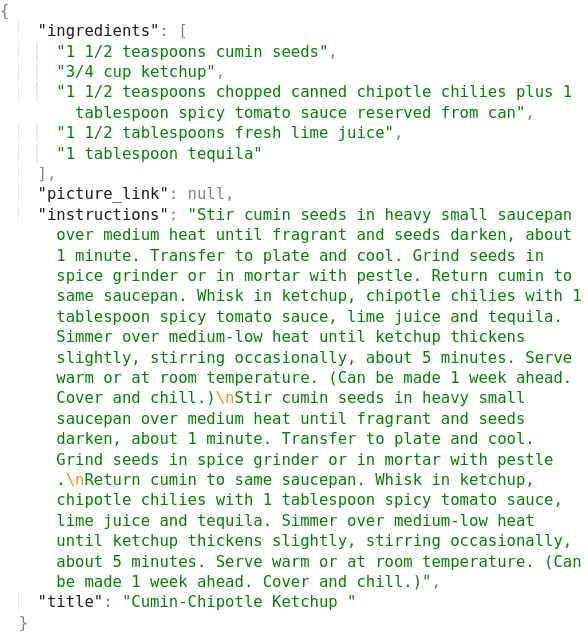
\includegraphics[width=0.75\textwidth]{imagenes/ejemplo-json-2.png}
    \caption{Estructura de las recetas en el dataset de archive.org}
    \label{fig:estructura-recetas}
\end{figure}

\subsection{Preprocesamiento de los datos textuales}\label{subsec:preprocessing}

Como se puede apreciar en la Figura \ref{fig:estructura-recetas}, los datos textuales de las recetas no se encuentran en un formato directamente manipulable para entrenar un modelo de lenguaje. Por ello, es necesario aplicar técnicas de preprocesamiento de datos que permitan su limpieza y adecuación para poder ser usados como datos de entrada en el entrenamiento del modelo de Word Embedding. En este paso, así como en todo el proceso de creación del modelo, haremos uso de la librería de Topic Modelling  Gensim\footnote{\url{https://radimrehurek.com/gensim/}}. Esta librería de código abierto proporciona funciones para trabajar con problemas de Procesamiento de Lenguaje Natural en el lenguaje de programación Python, y en particular, para entrenar y trabajar con modelos de Word Embedding. Con las funciones implementadas en dicha librería, podremos tanto entrenar como utilizar con facilidad el modelo, así como llevar a cabo las tareas de limpieza y preprocesamiento de los datos que utilicemos.

\subsubsection{Creación del corpus}

En primer lugar, hay que crear un corpus que recoja todos los datos textuales con los que se va a trabajar. Como ya se ha mencionado en secciones previas, los datos se encuentran distribuidos en cuatro ficheros, cada uno de ellos con una lista de las recetas obtenidas de los sitios web de recetas previamente mencionados. Por tanto, se requiere un preprocesamiento previo de cada uno de los ficheros correspondientes de forma que podamos disponer de una sola colección de datos que contenga únicamente la información textual que vamos a utilizar. Dicho de otra forma, debemos reestructurar la información para poder trabajar con un corpus con todos los datos textuales procedentes de los textos de preparación de las recetas que tenemos. 

Para solventar esta dificultad, se ha generado un fichero por cada receta con el texto de su preparación, de forma que únicamente trabajemos con ficheros cuyos datos son los que nos interesa preprocesar. De manera automatizada, se lee cada uno de los ficheros previamente generados para formar el corpus de recetas. En la Figura \ref{fig:creacion-corpus} se aprecia de forma esquematizada el procedimiento para montar este corpus.

\begin{figure}[H]
    \centering
  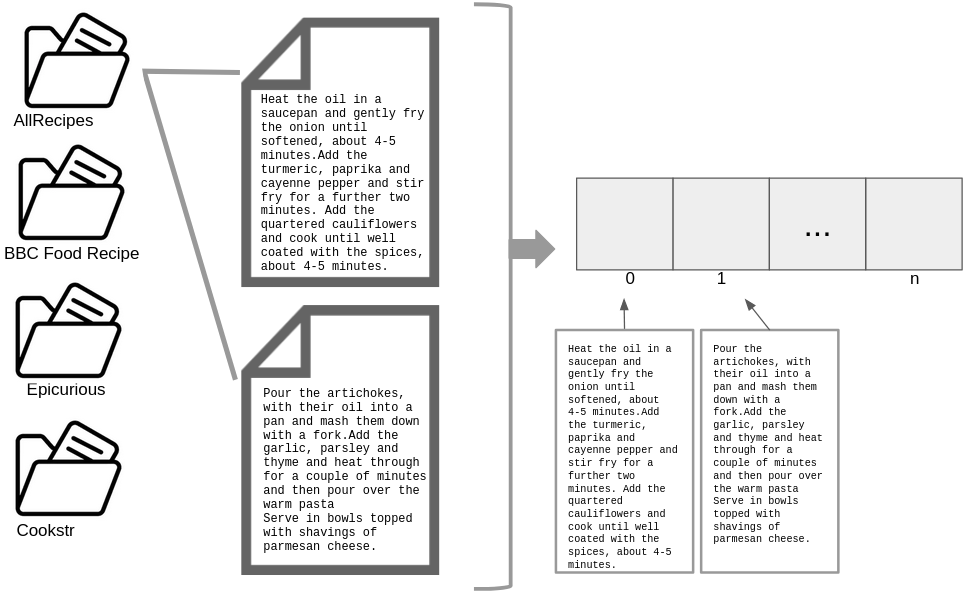
\includegraphics[width=0.8\textwidth]{imagenes/creacion-corpus-gris.png}
  \caption{Procedimiento para formar el corpus de recetas}
  \label{fig:creacion-corpus}
\end{figure}


\subsubsection{Limpieza del corpus}

Como se ha podido observar en ejemplos previos, el texto de preparación de las recetas se encuentra sin ningún tipo de procesamiento previo, y por ello necesita un tratamiento adecuado de la información textual para que el modelo de Word Embedding proporcione resultados de calidad. En nuestro caso, para el mencionado corpus de recetas se ha llevado a cabo la limpieza y tokenización que se presenta a continuación. Para complementar los pasos, utilizaremos como ejemplo el siguiente texto de preparación que se corresponde con una de las recetas del dataset: ``\texttt{Combine Ranch, salsa, tomatoes and chilies, if desired. Chill 1 hour. Serve with tortilla chips.}"

\begin{enumerate}
    
    \item \textbf{Tokenización del texto}. Se obtienen los tokens del fichero. Al generar los tokens se lleva a cabo la eliminación de símbolos (incluidos los de puntuación), dígitos, y pasar texto a minúsculas. Como resultado, se obtiene el texto como una lista de tokens con las palabras del fichero formadas por caracteres alfabéticos. Tras aplicar estos cambios, el ejemplo quedaría de la siguiente manera:
    
    \begin{center}
    
        \texttt{[`combine', `ranch', `salsa', `tomatoes', `and', `chilies', `if', `desired', `chill', `hour', `serve', `with', `tortilla', `chips']}
        
    \end{center}
    
    
    \item \textbf{Eliminación de las llamadas \textit{stopwords}}. Las stopwords son palabras muy comunes del vocabulario, que no van a proporcionar información útil, y por tanto es recomendable prescindir de ellas~\cite{saif2014stopwords}. Ejemplos de stopwords en inglés pueden ser ``the", ``a", ``my", ``your", etc. Para este caso, hemos utilizado la lista de stopwords en inglés proporcionada por la librería \textit{Gensim}. En este punto, el fichero tomado como ejemplo quedaría como se muestra a continuación:
    
    \begin{center}
        \texttt{[`combine', `ranch', `salsa', `tomatoes', `chilies', `desired', `chill', `hour', `serve', `tortilla', `chips']}
    \end{center}
    
    En el ejemplo se aprecia cómo se han eliminado aquellas palabras incluidas en el vocabulario de stopwords (en este caso, las stopwords existentes en el ejemplo son `\texttt{the}', `\texttt{if}'  y `\texttt{with}').\\
    

    \item \textbf{Aplicación de lematización}. Por último, aplicaremos una normalización lingüística al corpus conocida como lematización. Mediante esta técnica, se reducen todas las palabras a su raíz, de forma que se transforman las distintas variaciones morfológicas de una palabra a una única forma común. Esto ocurrirá, por ejemplo, con los verbos, donde nos encontraremos un mismo verbo en sus distintas formas verbales cuando todos ellos hacen referencia a una misma acción (así forzaremos a tener una única forma de aparición de los mismos). Tras aplicar la normalización comentada, el fichero quedaría de la siguiente forma:
    
    \begin{center}
        \texttt{[`combin', `ranch', `salsa', `tomato', `chili', `desir', `chill',  `hour', `serv', `tortilla', `chip']}
    \end{center}
    
    En dicho ejemplo se puede observar el caso comentado sobre los verbos, los cuales se han llevado a su raíz (como ocurre en el caso de `\texttt{serve}', que pasa a ser `\texttt{serv}'). También podemos ver que como resultado de dicha normalización se ha eliminado el plural de las palabras (`\texttt{tomatoes}' pasa a ser `\texttt{tomato}'). 
\end{enumerate}

\subsubsection{Detección de bigramas}
Por otra parte, en el lenguaje natural es normal que aparezcan palabras compuestas. El lenguaje culinario no es una excepción, y también existen palabras que suelen aparecer siempre juntas, como puede ser ``\textit{pimienta negra}", ``\textit{vino tinto}" o ``\textit{azúcar moreno}". Este tipo de casos, donde hay palabras que tienen más sentido ser tratadas como una sola que de manera independiente, da lugar al uso de técnicas de bigramas, que permiten tratar palabras (o en nuestro caso, tokens) de manera colectiva como si de una única se tratase. 

Para llevar esta idea a la práctica, en primer lugar es necesario entrenar el modelo de bigramas a partir de todos los textos que forman el corpus, para así poder detectar qué palabras son las que aparecen juntas una cantidad de veces considerable y poder representarlas en el texto como si fueran una sola. Esto se lleva a cabo sobre los datos una vez limpiados de la forma descrita en la sección anterior. Para este paso, también se ha hecho uso de las utilidades propocionadas por la librería Gensim. 

Una vez entrenado el modelo de bigramas, éste es aplicado sobre el mismo corpus para sustituir aquellos tokens de los que se detecten bigramas. A continuación se muestra cómo quedaría el ejemplo utilizado en el apartado anterior tras la detección de bigramas.

\begin{center}
    \texttt{[`combin', `ranch', `salsa', `tomato', `chili', `desir', `chill', `hour', `serv', `tortilla\_chip']}
\end{center}

Tal y como se puede ver, los token `\texttt{tortilla}' y `\texttt{chip}' pasarían a ser un token único (`\texttt{tortilla\_chip}'), lo cual es de esperar porque son dos palabras que, en las recetas, suelen encontrarse siempre juntas ya que se trata de un alimento cuya descripción textual es una palabra compuesta. 


\subsection{Implementación de Word2vec}\label{subsec:implementacion}
Para construir el modelo lingüístico a partir del corpus de recetas descrito en las secciones anteriores se pueden utilizar distintos algoritmos no supervisados estandarizados. Entre los más conocidos, se encuentran Word2Vec~\cite{mikolov2013distributed, mikolov2013efficient}, Glove~\cite{pennington2014glove} o fasttext~\cite{bojanowski2016enriching}. 
En este trabajo, se ha optado por utilizar el algoritmo Word2vec para entrenar el Word Embedding. De este algoritmo existen diferentes implementaciones; las más conocidas son las denominadas \textit{Continuous Bag of Words} and \textit{Skip-Gram} \cite{rong2014word2vec}. A continuación, se explica de forma detallada en qué consisten estas implementaciones. 

\subsubsection{Modelo Continuous Bag of Words (CBOW)}
Esta implementación de Word2vec se centra en predecir una palabra a partir del contexto, cuya estructura puede apreciarse en la Figura \ref{fig:cbow-1}. La capa de entrada de la red ($X$) representará el contexto, la capa oculta ($H)$ hace referencia al Embedding entrenado y la capa salida ($Y$) representará la palabra de la que se quiere obtener su representación en el modelo. Este contexto puede estar formado por una o más palabras. En el caso de que el contexto esté formado por una única palabra, estaríamos en la versión simplificada de este modelo (que es la mostrada en la Figura \ref{fig:cbow-1}). Independientemente del tamaño tenido en cuenta en el contexto, cada una de las palabras que formen parte del mismo se encuentran codificadas mediante el método \textit{one-hot-enconding} explicado en secciones anteriores. Este vector tendrá como tamaño el del vocabulario (notado por $V$), y estará completo a valor 0 exceptuando las posiciones que se correspondan con la palabra (o palabras) que se utilicen en el contexto, cuyo valor será 1.

% enos uno de sus elementos, cuyo valor será 1. Este elemento será el correspondiente a la palabra del vocabulario que coincida con la palabra del contexto que se quiera codificar en ese momento. Dicho de otra forma, la codificación de una palabra del contexto identificada en el vocabulario del modelo como $v_i$, se codificará como el vector $X$, de tamaño $V$. Dicho vector $X$ tendrá valor 0 en todos sus elementos, a excepción del elemento $X_i$ el cual tendrá valor 1.
    
\begin{figure}[H]
    \centering
    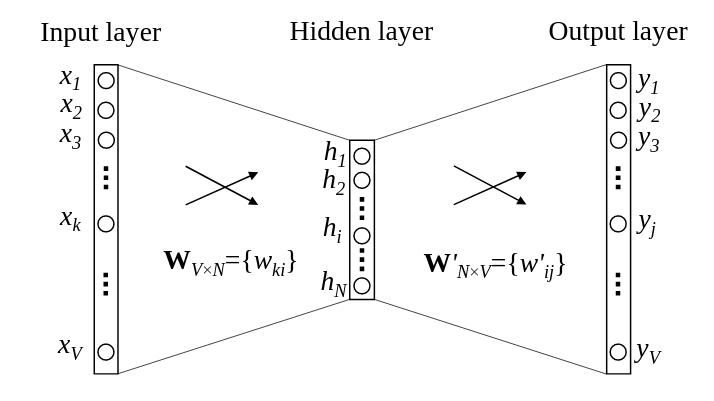
\includegraphics[width=0.65\textwidth]{imagenes/cbow_esquema.png}
    \caption{Modelo CBOW donde el contexto es una palabra~\cite{rong2014word2vec}}
  \label{fig:cbow-1}
\end{figure}
    
\subsubsection{Modelo Skip-Gram}
En este modelo, se lleva a cabo el procedimiento inverso. A pesar de que la capa oculta ($H$) sigue representando el Embedding, en este caso, la capa de entrada del modelo ($X$) es la palabra que corresponde a la capa de salida en el modelo CBOW (es decir, el target). Tal y como se puede ver en la Figura \ref{fig:modelos-w2v}b, la capa de salida ($Y$) de este modelo está formada por el contexto correspondiente a la palabra proporcionada como entrada. En otras palabras, mientras que en el modelo CBOW lo que se predice es la palabra, en el modelo Skip-Gram lo que se pretende predecir es el contexto de dicha palabra. En la selección de Figuras \ref{fig:modelos-w2v} se puede ver de forma gráfica esta diferencia existente entre los modelos. 

\begin{figure}[h!]
    \centering
    \begin{subfigure}[b]{0.47\textwidth}
        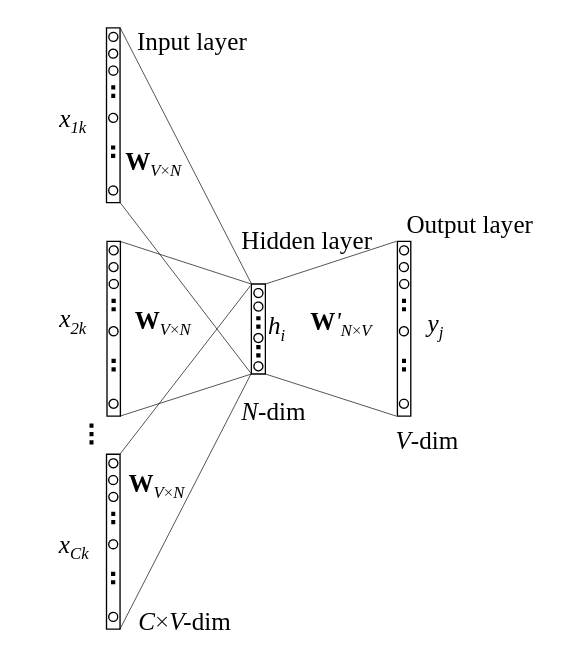
\includegraphics[width=1.0\textwidth]{imagenes/cbow_esquema2.png}
        \caption{Modelo CBOW}
    \end{subfigure}
    \begin{subfigure}[b]{0.47\textwidth}
        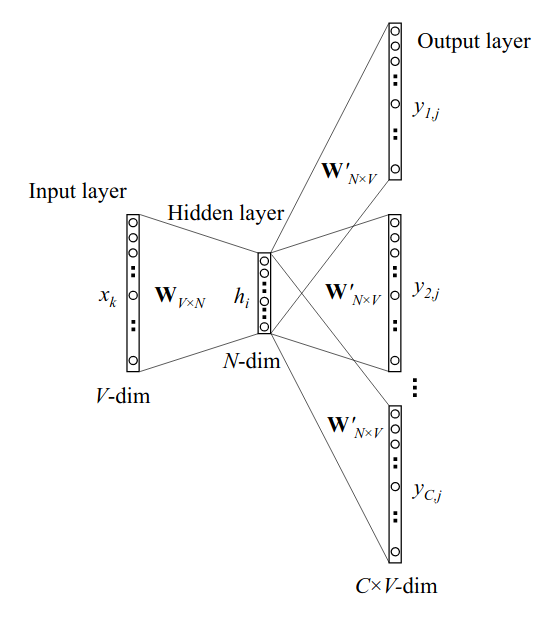
\includegraphics[width=1.0\textwidth]{imagenes/skipgram_esquema.png}
        \caption{Modelo Skip-gram.}
    \end{subfigure}
    \caption{Modelos del algoritmo Word2vec~\cite{rong2014word2vec}}
    \label{fig:modelos-w2v}
\end{figure}


Como es de esperar, ambos modelos tienen sus ventajas y desventajas, y cada uno de ellos es más o menos apropiado en función del problema en cuestión. En líneas generales, el modelo CBOW suele funcionar mejor con palabras del vocabulario que aparecen con frecuencia, mientras que Skip-Gram es capaz de obtener buenas representaciones para vocabulario poco frecuente en el corpus utilizado para entrenar el modelo de Word Embedding. 

\subsection{Entrenamiento del modelo}\label{subsec:train}
Para el entrenamiento del modelo de Word Embedding a partir del corpus de recetas hemos decidido utilizar la implementación de Word2vec \textit{Continuous Bag of Words} (CBOW). La razón principal reside en su implementación, que permite obtener buenas representaciones para palabras de uso frecuente. Esto es especialmente adecuado para nuestro problema dado que en el vocabulario culinario hay una gran cantidad de palabras que aparecen con mucha frecuencia en los textos. Al igual que con la creación del corpus y su preprocesamiento, hemos utilizado las funcionalidades de la librería Gensim para llevar a cabo el entrenamiento del modelo. En el Capítulo \ref{ch:Pruebas} se detalla la experimentación y el ajuste de hiperparámetros realizado.

\chapter{Mapeo de datos}
% mapping entre elementos heterogéneos 

\label{ch:Capitulo 6}

\begin{quote}
  Este capítulo presenta el procedimiento y las distintas medidas implementadas para calcular la similitud entre dos descripciones de forma que podamos distinguir cuándo dos elementos son equivalentes.
\end{quote}


\section{Procedimiento de mapeo}

Ser capaces de identificar un alimento en una base de datos de composición nutricional es una tarea esencial si queremos realizar algún tipo de tarea automática que conlleve consultar valores nutricionales de alimentos o ingredientes en recetas. Esta tarea se puede simplificar a la decisión de si dos alimentos son equivalentes o no en función de lo parecidas que sean sus descripciones nutricionales.

Para conocer la similitud entre dos descripciones textuales de alimentos se han implementado distintas medidas de distancia, detalladas en la Sección~\ref{sec:proced_mapeo}. Con dichas medidas de distancia, se permitirá mapear alimentos entre bases de datos con el objetivo de identificar equivalencias y agregar sus atributos. Para poder llevar a cabo esta identificación, es necesario conocer la distancia de la descripción textual del ingrediente en respecto a las descripciones de los posibles alimentos hacia los que podamos realizar el emparejamiento. El mapeo más adecuado (y el que finalmente devuelve la herramienta como alimento equivalente) será aquel con el obtengamos la distancia mínima de entre todos los alimentos de la base de datos a mapear. De esta forma, cuanto más cercano a 0 sea el valor de distancia entre dos alimentos dados, más parecidos serán esos alimentos y viceversa. Finalmente, elegiremos la medida que mejor se ajuste a las funcionalidades del sistema implementado, en función del resultado obtenido con cada una de ellas.

Es importante recalcar, que estas descripciones no tienen por qué corresponderse con una única palabra; en algunos casos sí lo será (p.ej., \textit{patata} o \textit{zanahoria}) pero en otros casos, la descripción del ingrediente puede ser más extensa (p.ej., \textit{pimiento asado en conserva} o \textit{salsa mahonesa reducida en calorías)}. Por ello, cada una de estas descripciones va a ser tratada como un documento corto, formado únicamente por dicha descripción. Con esta consideración, podremos tener en cuenta toda la información de la descripción del ingrediente, tanto de una forma global, como de manera individual con las palabras que lo forman. Manteniendo la coherencia con la implementación del modelo de Word Embedding, a las descripciones textuales se les debe aplicar previamente las tareas de preprocesamiento y limpieza de datos detalladas en el Capítulo \ref{ch:Capitulo 5}. Por ello, en este punto hablaremos de \textit{token} en lugar de \textit{palabra}, como forma de referirnos al contenido de la descripción correctamente procesado.


\section{Medidas de distancia implementadas}\label{sec:proced_mapeo}

Sea $S_{i}$ la descripción textual correspondiente a un alimento, y sea  $T_{i}=\lbrace t_{1},...,t_{n}\rbrace$ el conjunto de tokens obtenido como resultado de las tareas de preprocesamiento aplicadas a dicha descripción. Por ejemplo, consideremos el elemento $k$ con la representación textual  $S_{k}$=\textit{``Canned  fish, average"}. Su conjunto $T_{k}$ correspondiente sería $\lbrace \textit{``can", ``fish", ``average'' } \rbrace $. Teniendo en cuenta esta nomenclatura, se han implementado distintas medidas de distancia entre descripciones textuales de alimentos, detalladas a continuación.


\subsection{Distancia sintáctica entre descripciones}
    
En primer lugar, se ha optado por implementar una medida de distancia basada en la concordancia entre dos descripciones textuales, que nos permita distinguir si dos descripciones son más parecidas o no en base a la comparación a nivel de caracteres de su representación textual.

\subsubsection{Distancia de Jaccard}
La distancia de Jaccard (ver Fórmula \ref{formula:jaccard}) permite medir el grado de intersección entre dos conjuntos~\cite{wang2011fast}. En este caso, cada descripción alimenticia formará un conjunto, y los tokens de dicha descripción serán los elementos de dicho conjunto. Esta medida devuelve un valor comprendido entre 0 y 1, donde el 0 hace referencia a dos conjuntos iguales mientras que el 1 a dos conjuntos totalmente disjuntos. Este valor es calculado a partir de la intersección entre ellos. Para poder medir el grado de la intersección de los conjuntos, se debe determinar cuáles, de entre todos los elementos de dos conjuntos dados, pertenecen a la intersección de ambos. Para que uno de los tokens forme parte de la intersección de dichos conjuntos, debe aparecer de forma exacta en ambos conjuntos. En nuestro caso, dos elementos pertenecerán a la intersección en función del parecido léxico entre ellos.

\begin{align}
\label{formula:jaccard}
    J(S_{1},S_{2})=1-\frac{\left | T_{1} \cap T_{2}\right |}{\left | T_{1} \right |+\left | T_{2} \right |-\left | T_{1}\cap T_{2} \right |} 
\end{align}

Para ver el funcionamiento de esta medida de distancia, se va a mostrar como ejemplo la medida de distancia de Jaccard entre dos descripciones textuales de alimentos $S_1$ y $S_2$, que se corresponden con \texttt{`Coconut oil'} y \texttt{`Palm seed oil'} respectivamente.
En la Figura \ref{fig:jaccard}a, se aprecia cómo quedarían representados como conjuntos las descripciones denotadas por $S_1$ y $S_2$. En dicha imagen se puede ver cómo la descripción \texttt{`Coconut oil'} se representa como un conjunto con dos elementos: \texttt{coconut} y \texttt{oil}, mientras que \texttt{`Palm seed oil'} se representa como conjunto formado por tres elementos (\texttt{palm}, \texttt{seed} y \texttt{oil}). En la Figura \ref{fig:jaccard}b se puede ver la intersección entre los dos conjuntos. Como se puede observar, el conjunto intersección está formado por un único elemento, \texttt{oil}, el cual es el único que aparece en ambos documentos (y por tanto en sus conjuntos). Aplicando sobre estos conjuntos la medida de Jaccard expuesta en la Fórmula \ref{formula:jaccard}, obtendríamos que la distancia entre ambos conjuntos es $J(S_{1},S_{2})=1-\frac{1}{2+3-1} = 0.75$.



\begin{figure}[h!]
    \centering
    \begin{subfigure}[b]{0.47\textwidth}
        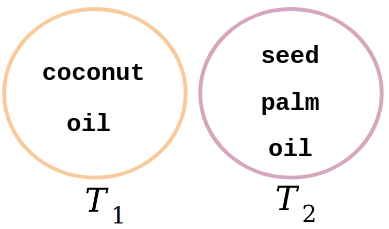
\includegraphics[width=1.0\textwidth]{imagenes/img1.png}
        \caption{Documentos representados como conjuntos}
    \end{subfigure}
    \hspace{5mm}
    \begin{subfigure}[b]{0.47\textwidth}
        \centering
        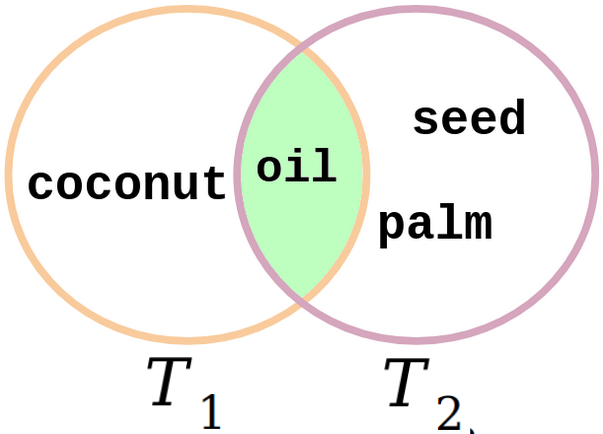
\includegraphics[width=0.80\textwidth]{imagenes/img5.png}
        \caption{Intersección entre los conjuntos de esos documentos}
    \end{subfigure}
    \caption{Intersección entre dos conjuntos}
    \label{fig:jaccard}
\end{figure}





\subsubsection{Distancia Levenshtein}
La distancia de Levenshtein es otra medida de concordancia entre descripciones textuales, y se define como el mínimo número de operaciones o movimientos que son necesarios para transformar una secuencia de caracteres en otra~\cite{yujian2007normalized}. Esta medida de distancia permite tanto trabajar de forma normalizada (por ejemplo, en el rango 0 a 1) como sin normalizar. 

Aplicada a nuestro problema en cuestión, hace referencia al número de movimientos necesarios para pasar de la descripción de un ingrediente a la de otro. Los movimientos permitidos vienen enumerados a continuación:

\begin{itemize}
    \item Eliminar un carácter: ABC $\xrightarrow{}$ AB, AC, BC
    \item Añadir un nuevo carácter: ABC $\xrightarrow{}$ ABCD, EABC, AEBC
    \item Sustituir un carácter por otro: ABC $\xrightarrow{}$ ABE, ADC, FBC
\end{itemize}


\subsection{Distancia semántica entre descripciones}

En este caso, se ha optado por una medida de distancia que utilice la representación numérica obtenida por el modelo de Word Embedding. Dado que esta representación se obtiene utilizando el contexto de cada palabra, trae de forma implícita la representación de su semántica. El utilizar medidas de distancia entre las representaciones numéricas de las palabras (o documentos) nos permitirá detectar si dos palabras son más o menos parecidas en función del contexto en el que se usen. 



\subsubsection{Distancia Word Mover's}

La medida de distancia Word Mover's trata los documentos cortos como representaciones de una nube de puntos, donde cada punto representa una palabra del documento expresada de forma vectorial a partir del modelo de Word Embedding. La distancia entre dos nubes se cuantifica como el coste que las palabras de un documento de texto deben asumir para coincidir exactamente con la nube de puntos del otro documento de texto~\cite{kusner2015word}. En nuestro caso, cada descripción alimenticia formará un documento corto.

\begin{figure}[H]
    \centering
    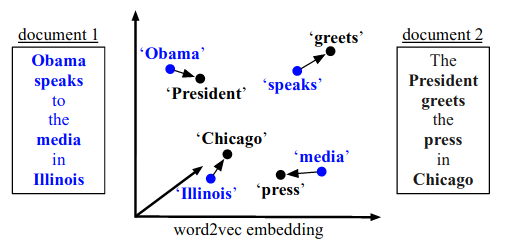
\includegraphics[width=0.7\textwidth]{imagenes/wmd.png}
    \caption{Funcionamiento de la distancia Word Mover's ~\cite{kusner2015word}}
    \label{fig:wmd}
\end{figure}

Para calcular la distancia entre dos palabras individuales, se utiliza una distancia euclídea entre las representaciones vectoriales correspondientes. De esta forma, se mantiene la semántica a la hora de obtener la similitud entre las palabras. En la Figura \ref{fig:wmd} se puede apreciar de manera gráfica el funcionamiento de esta medida de distancia. 

    
\subsection{Distancia híbrida entre descripciones}

En los apartados anteriores se han detallado medidas de distancias que tienen en cuenta la distancia entre descripciones desde un punto de vista puramente léxico o desde una aproximación basada en la semántica. 

Con el objetivo de obtener una mayor precisión en los resultados, se introduce una medida híbrida que tiene como objetivo combinar la capacidad sintáctica y la semántica de las descripciones textuales. Esta función de distancia se formula como una combinación ponderada de las distancias de Jaccard y Word Mover's (ver Fórmula~\ref{formula_hi}). Con esta medida, se pretende beneficiar aquellas descripciones textuales que sean similares desde un punto de vista sintáctico, sin olvidar la importancia de la semántica a la hora de alcanzar el resultado más preciso posible. 

    \begin{equation}
        HDISTANCE(t_{1},t_{2})=wJ(t_{1},t_{2}) + (1-w)WMD(t_{1},t_{2})
     \end{equation}
    \begin{center}
    donde $w\in {\rm I\!R}$ and $0 \leq w \leq 1$
    \end{center}\label{formula_hi}


\subsection{Fuzzificación de las medidas de distancia }
Cuando se trabaja con datos textuales, una de las cosas que hay que tener en cuenta es que hay que hacer frente a los problemas derivados de la ambigüedad del lenguaje. En capítulos anteriores ya se ha introducido la importancia de la semántica en el tratamiento de datos textuales. Esta importancia viene derivada de dificultades comunes que suelen aparecer al trabajar con información textual, como puede ser el uso de sinónimos, palabras muy similares, o incluso hacer frente a distintos niveles de detalle en las descripciones con las que trabajamos. 

Para lidiar con esta vaguedad existente en el lenguaje, se ha propuesto implementar medidas de distancia con Lógica Difusa que permitan dotar a nuestra herramienta de una mayor flexibilidad y robustez para hacer frente a este tipo de desafíos. En concreto, se han fuzzificado dos medidas de las detalladas en este capítulo, que se corresponden con Jaccard y Word's Mover. En ambas medidas se parte de la descripción textual como un conjunto de tokens, que se corresponden con la lista de palabras que forman la descripción textual a las cuales se les ha aplicado las tareas de preprocesamiento explicadas en el capítulo anterior. 



%The latter, along with the vagueness associated to the language (e.g., a mapping of two equivalent items with different level of specialization) calls for flexible approaches to calculate the mappings.

\subsubsection{Distancia difusa de Jaccard}
En este capítulo, se ha explicado el funcionamiento de la medida de distancia de Jaccard, la cual computa la distancia en base a la cantidad de elementos que forman parte de la intersección entre conjuntos. Dicha medida establece la intersección de forma estricta: un elemento pertenece al conjunto intersección solo si se encuentra de manera exacta en ambos conjuntos. Teniendo esto en cuenta, la medida de Jaccard no contempla que dos elementos similares se valoren a la hora de medir la similitud entre dos conjuntos.

Por la ambigüedad existente en el lenguaje y las múltiples formas de expresar una descripción alimenticia, se ha optado por implementar una versión difusa de la medida de Jaccard, que permita tener en cuenta el parecido entre los elementos de ambos conjuntos de manera proporcional al grado de similitud que tengan. De esta forma se valorará de forma positiva el parecido léxico entre los elementos que, sin llegar a formar parte de la propia intersección, sí tienen un grado de parecido notable que incita a ser considerados en el cálculo de la medida de distancia.

\begin{figure}[h!]
    \begin{subfigure}[b]{0.47\textwidth}
        \centering
        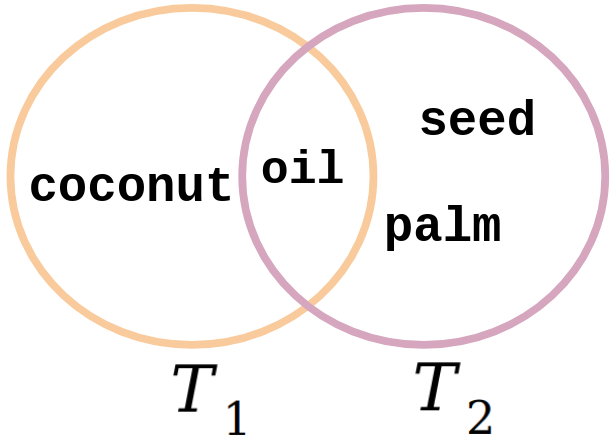
\includegraphics[width=0.8\textwidth]{imagenes/img2.png}
        \caption{Intersección clásica}
    \end{subfigure}
    \begin{subfigure}[b]{0.47\textwidth}
        \centering
        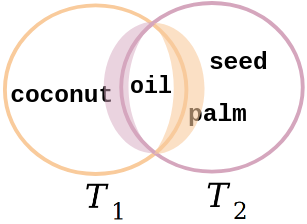
\includegraphics[width=0.78\textwidth]{imagenes/img3.png}
        \caption{Intersección difusa}
    \end{subfigure}
    \caption{Intersección entre dos conjuntos}
    \label{fig:jaccard_difuso}
\end{figure}

La versión difusa de Jaccard implementada se aprecia en la Fórmula \ref{formula:jaccard_fuz}~\cite{wang2011fast}. Consiste en una combinación de similitudes tanto a nivel de token como de carácter, con el objetivo de determinar el conjunto de intersección difusa que existe entre dos conjuntos (entendiendo cada descripción textual como un conjunto). Para conocer la distancia a nivel de token se utiliza la medida Jaccard que se ha descrito anteriormente, y mediante un umbral $\delta$ se determina cuáles de estos tokens forman parte del conjunto de intersección difuso. El valor del umbral se ha ajustado empíricamente al valor de 0.2. 

\begin{equation}
    \label{formula:jaccard_fuz}
    \tilde{J}_{\delta}(S_{1},S_{2})=\frac{\left | T_{1} \tilde{\cap}_{\delta} T_{2}\right |}{\left | T_{1} \right |+\left | T_{2} \right |-\left | T_{1}\tilde{\cap}_{\delta} T_{2} \right |}
\end{equation}
\begin{center}
    $\delta=0.2$
\end{center}

Para ilustrar el cálculo de esta medida, vamos a usar el mismo ejemplo que se empleó para la medida Jaccard (ver Figura \ref{fig:jaccard}) para ejemplificar cómo funciona su versión difusa. En la Figura \ref{fig:jaccard_difuso} se puede ver el valor de distancias a nivel de token entre ambos conjuntos.  Por simplificación, únicamente se muestran aquellas distancias cuyo valor es distinto de 1, y que por tanto, tienen alguna posibilidad de poder formar parte de la intersección difusa. En este caso, las líneas continuas, representan aquellos elementos cuya medida de distancia supera el umbral y por tanto se incluyen en la intersección difusa. Como se puede ver, en este caso el único elemento que lo supera es \texttt{oil}, por lo que la intersección tradicional y la difusa serían la misma: $J(S_{1},S_{2})=1-\frac{1}{2+3-1} = 0.75$.

\begin{figure}[H]
    \centering
    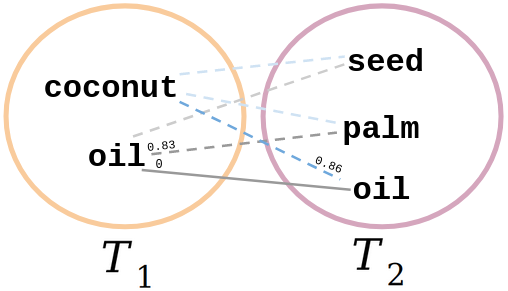
\includegraphics[width=0.7\textwidth]{imagenes/img4.png}
    \caption{Función de distancia difusa Jaccard}
    \label{fig:fuzzy_jaccard_metric}
\end{figure}


Ahora imaginemos que, en un hipotético caso, la distancia entre \textit{coconut} y \textit{palm} es 0.1 porque son extremadamente similares, y por tanto entraría dentro del conjunto de la intersección difusa al no superar el umbral. Si aplicamos la fórmula de la distancia difusa de Jaccard, se quedaría tal que $J(S_{1},S_{2})=1-\frac{1+0.9}{2+3-1-0.9} = 0.39$, un valor inferior que el obtenido con la versión clásica, que sí representaría esta valoraría la similitud entre los elementos.

\subsubsection{Distancia difusa entre documentos}
Se ha diseñado una medida de la distancia entre documentos cortos partiendo de un enfoque difuso, considerando cada documento como el conjunto de tokens que se obtienen del preprocesamiento de la descripción textual.

En las medidas que trabajan con conjuntos que se han utilizado hasta ahora, (entre ellas incluida la medida difusa de Jaccard) se hace hincapié en el parecido de los elementos entre conjuntos uno a uno. Sin embargo, parece interesante medir la distancia de un elemento a un conjunto completo, en lugar de distancia entre elemento y elemento. Esto permitiría obtener una medida que valore el papel de cada elemento al nivel de la descripción textual, y no elemento a elemento lo cual podría resultar poco apropiado, puesto que no se estaría teniendo en cuenta a la descripción como un todo. Por ello, se ha propuesto en este trabajo la medida de distancia $\tilde{D}$, la cual se centra en esta afirmación y cuyo cálculo se expone en la Fórmula \ref{formula:fuzzy-document}. Para poder obtener el valor de distancia $\tilde{D}$ entre las descripciones textuales $S_{1}$ y $S_{2}$ se tienen en cuenta los siguientes puntos:

\begin{enumerate}
    \item Obtener el conjunto unión ($T_{1}\cup T_{2}$) de los conjuntos $T_{1}$ y $T_{2}$ , los cuales se corresponden respectivamente con el conjunto de tokens que forman las descripciones $S_{1}$ y $S_{2}$. %AÑADIR EJEMPLOS
    
    \item Calcular, para cada elemento presente en los conjuntos $T_{1}$ y $T_{2}$ (el cual se encuentra en el conjunto $T_{1}\cup T_{2}$) su grado de pertenencia al conjunto contrario. Para calcular el grado de pertenencia de un elemento a un conjunto, se utiliza la función $\mu_{T_{i}}(x)$, donde $i$ hace referencia al conjunto y $x$ al elemento del que se quiere obtener el grado de pertenencia a dicho conjunto $i$.
    

    \item Calcular el valor de la intersección difusa de los dos conjuntos. Para calcular el grado de pertenencia de un elemento a un conjunto, se utiliza la función $\mu_{T_{i}}(x)$ comentada en el punto anterior.
    \item El valor de distancia se corresponde con el resultado de la sumatoria en el paso 2 dividido entre el valor de la intersección en el paso 3.
\end{enumerate}

Como se puede apreciar en el cálculo de dicha medida, se hace uso de la función de pertenencia $\mu_{T_{i}}(x)$ la cual permite obtener el grado de pertenencia del elemento $x$ al conjunto $T_{i}$, donde $x$ hace referencia a un elemento de un conjunto obtenido a partir de una descripción textual, y  $T_{i}$ es el conjunto que representa a la descripción textual $S_{i}$.

\begin{equation}
\label{formula:fuzzy-document}
   \textstyle \tilde{D}(S_{1},S_{2})=\frac{\sum_{x\epsilon T_{1}\cup T_{2} }min(\mu T_{1})x \times min(\mu T_{2})x}{\sum_{x\epsilon T_{1} }(\mu T_{1} )(x)+\sum_{x\epsilon T_{2} }(\mu T_{2} )(x)-\sum_{x\epsilon T_{1}\cup T_{2} }min(\mu T_{1})x \times min(\mu T_{2})x}  
\end{equation}\label{for:pertenencia}
    

\begin{equation}
\label{formula:fuzzy-document-2}
\mu_{T_{i}}(x)= \left\{ \begin{array}{lcc}
         1 &   & d_{E}(t_{i},x) = 0 \\
         \\ 0 &   &  d_{E}(t_{i},x) = \infty \\
         \\ sigmoid(\frac{1}{d_{E}(t_{i},x)}) &    & 0 < d_{E}(t_{i},x) < \infty 
         \end{array}
\right .   
\end{equation}
\begin{center}
    donde $d_{E}(t_{i},x)$ es la distancia euclídea entre $t_{i}$ y $x$
\end{center}
    
En la práctica, al determinar el grado de pertenencia de un elemento a un conjunto, estamos haciendo referencia al parecido entre los elementos de descripciones. Para ello, se ha diseñado una función de pertenencia, la cual se puede observar en la fórmula Fórmula \ref{for:pertenencia}. Para la definición de esta función, En primer lugar hay que determinar la medida de distancia entre dos elementos textuales procedentes de descripciones. En este caso, la distancia entre dos elementos o tokens procedentes de las  descripciones se calcula como la distancia euclídea entre los vectores de los tokens de ambos conjuntos. Estos vectores corresponden a la representación numérica obtenida del modelo de Word Embedding previamente entrenado. En función del resultado que se obtenga con la distancia euclídea, se consideran tres casuísticas, las cuales se contemplan en la función de pertenencia:

\begin{enumerate}
    \item Si el valor de distancia euclídea entre los vectores de dos palabras del vocabulario es 0, las dos palabras son idénticas, por lo que el grado de pertenencia es máximo. En nuestro caso, este valor es 1 y representa la máxima similitud. Esta situación se encuentra contemplada en el primer caso de la función de pertenencia (ver fórmula \ref{formula:fuzzy-document}).
    
    \item El segundo caso contemplado en la función de pertenencia (ver fórmula \ref{formula:fuzzy-document}) hace referencia a aquellas situaciones donde el valor de distancia euclídea sea $\infty$. Que se obtenga dicho valor significa que no se ha podido determinar la distancia entre elementos porque no se tiene representación vectorial de alguno de ellos, o incluso de ambos. En este caso al no poder determinarse un valor de distancia, no hay pertenencia posible y como resultado, el grado de pertenencia es 0, que representa similitud nula.
    
    \item Si el valor de distancia euclídea se encuentra en el intervalo $(0,\infty)$, estamos en el último caso contemplado por la función de pertenencia. Puesto que estamos trabajando con grados de pertenencia, para poder acotar el problema debemos trasladar este valor de distancia al intervalo (0,1). Para ello, se ha utilizado el valor de la función \textit{sigmoide} de la inversa de la distancia. Con este cálculo, conseguimos trabajar con valores acotados en el intervalo (0,1) que representen la similitud entre dos elementos. 
\end{enumerate}


Con esta medida, se premia a aquellos elementos que aparecen en ambos conjuntos, a la vez que se combina con el parecido existente entre los tokens que no forman parte de la intersección. Además, con la función de pertenencia utilizada se tiene en cuenta la carga semántica que contempla el modelo de Word Embedding descrito en la sección anterior, dotando así de una mayor flexibilidad a la herramienta. 

\section{Elección de la medida de distancia}

Para analizar el funcionamiento de este módulo y evaluar la calidad de los resultados obtenidos con las distintas métricas, se ha estudiado el comportamiento de cada una de las medidas expuestas en la sección anterior aplicando este módulo a un problema de mapeo de datos entre dos bases de datos de composición nutricional, detallado en el Capítulo \ref{ch:Pruebas}. El objetivo de esta tarea de mapeo de datos es estudiar cómo se comportan las distintas medidas de distancia utilizadas, y poder concluir cuál de ellas se adapta mejor al problema y es capaz de identificar elementos equivalentes con mayor precisión. 


\chapter[Diseño y desarrollo de la aplicación]{Diseño y desarrollo de la aplicación para adaptación de recetas}
\label{ch:Consultas_Adaptadas}

\begin{quote}
  Este capítulo recoge el comportamiento del módulo de Consultas adaptadas, así como la descripción del prototipo de aplicación que se ha implementado para ilustrar el funcionamiento del sistema de adaptación de dietas con la herramienta de fusión de datos heterogéneos.
\end{quote}


\section{Recomendación de recetas}

La recomendación de las recetas es un campo concreto de estudio dentro de los sistemas de recomendación en Food Computing, el cual se centra fundamentalmente en la recomendación de dietas cuyas recetas cumplen una serie de características nutricionales. Entre otras muchas especificaciones, destacan las dietas saludables o aquellas que persiguen un objetivo concreto, como puede ser la pérdida de peso o la definición de masa muscular.

Dentro del amplio campo de estudio de recomendación de recetas, destacan dos formas principales: la recomendación de recetas ya existentes, y la recomendación de recetas a partir de generación automática de recetas~\cite{chen2019eating}. En el primer caso hablamos de recomendación de recetas ya existentes donde los sistemas, en base a unas preferencias concretas, realizan un filtrado hasta proporcionar la receta o conjunto de ellas que mejor se adapten a los requerimientos del usuario. Se han desarrollado una gran cantidad de sistemas de recomendación basados en recetas desde el punto de vista de Recomendación basada en el contenido, en función de  la puntuación y opinión que los usuarios tienen de los ingredientes que las forman~\cite{Freyne:2010:IFP:1719970.1720021,a3e625bf40904a799c3b8e35929388b7}.
En cuanto a los sistemas de recomendación dependiente del contexto, se han desarrollado sistemas que aconsejan recetas en base al género, tiempo, aficiones, localización u otros aspectos culturales relacionados con los usuarios. También hay distintos sistemas de recomendación que tienen en cuenta distintas combinaciones de sabores, o incluso patrones de combinación de ingredientes en las distintas recetas, y otros basados en otro tipo de datos que en principio puedan parecer menos relevantes, como la rutina diaria de usuarios obtenida a partir de redes sociales como Twitter~\cite{Rokicki2016PlateAP}. En el segundo caso hablamos de sistemas generadores de recetas automáticas: a partir del estudio de las relaciones que existen entre ingredientes, recetas y factores multiculturales en las cocinas, se pueden generar versiones de recetas que permitan mantener dicha coherencia intrínseca contenida en las recetas~\cite{10.3389/fict.2018.00014}. En este capítulo, nos centramos en este segundo caso.


Además, es relevante destacar que la incorporación de aspectos saludables en los sistemas de recomendación de dietas tiene especial importancia, y, debido a la gran cantidad de literatura centrada en la incorporación de este factor a los sistemas de recomendación, merece ser destacada en este apartado. En los últimos años, se ha producido un auge en el desarrollo de sistemas de recomendación centrados en la generación automática de dietas personalizadas teniendo como requisito que sean saludables~\cite{burilo2019nutricion,Trattner2017}. 



\subsubsection{Aplicaciones móviles de recomendación de recetas}

Utilizar aplicaciones móviles para resolver problemas de Food Computing ha resultado exitoso, mostrando su efectividad en ensayos focalizados a la adecuación del consumidor hacia dietas más saludables~\cite{ipjian2017smartphone}. Los sistemas de Food Computing cada vez se encuentran más inmersos en las aplicaciones móviles, dando lugar a múltiples aplicaciones con funcionalidades muy diversas. El desarrollo de las comunidades de usuarios online en las que se comparten millones de recetas (AllRecipes y Yummly) ha contribuido a la disponibilidad de su información a través de aplicaciones móviles más allá de mantener su servicio vía web. Sin embargo, estos servicios están muy focalizados a la búsqueda de recetas, y no a su recomendación y adaptación a los usuarios, lo cual es una de las funcionalidades más demandadas desde estas aplicaciones~\cite{chen2019eating}. En esta línea, han surgido sistemas centrados en la recomendación de recetas a través de dispositivos móviles~\cite{cheng2014content,johnson2014mobile,ketmaneechairat2017recommender,maruyama2012real}. 

La falta de información (normalmente nutricional) muy concreta o específica que se suele proporcionar en las recetas procedentes de esas fuentes de datos ha originado que éstas no tenga cabida en que los sistemas de recomendación de recetas ya existentes, ya que las características de estos conjuntos de datos no son lo suficientemente detalladas como para poder trabajar con restricciones muy específicas que no se proporcionen en ámbitos poco especializados. Es por ello que la generación y completación de recetas ha sido y es la vía de recomendación de recetas más utilizada en este ámbito, utilizando para ello las relaciones existentes entre ingredientes y recetas~\cite{de2016data}. En este contexto podemos destacar el framework \textit{NutRec}, cuyo motor principal en un sistema de recomendación basado en la búsqueda de recetas similares a una pseudo-receta generada automáticamente a partir de las especificaciones concretas del usuario.

\section{Adaptación de recetas según restricciones}

Como ya se ha ido introduciendo a lo largo del desarrollo de este proyecto, para ilustrar el funcionamiento del sistema desarrollado se ha implementado un módulo de Consultas Adaptadas, el cual, en nuestro caso, permite adecuar recetas en función de unas restricciones alimenticias dadas. Para ello, se permite seleccionar una receta y una restricción con el objetivo de detectar sus ingredientes y modificarlos en caso de que la información nutricional de alguno (o varios) de ellos impida su uso en en algún tipo de dieta (como puede ser la vegetariana). 

En este último módulo del sistema se hace uso de fuentes de datos heterogéneas que se fusionan mediante los dos módulos anteriores explicados en el Capítulo \ref{ch:Capitulo 5} y \ref{ch:Capitulo 6}. De esta forma, con una única consulta podremos obtener todos los datos necesarios para que este módulo pueda funcionar correctamente. En la Figura \ref{fig:datos-agregados} se visualiza esta misma idea.

\begin{figure}[H]
    \centering
    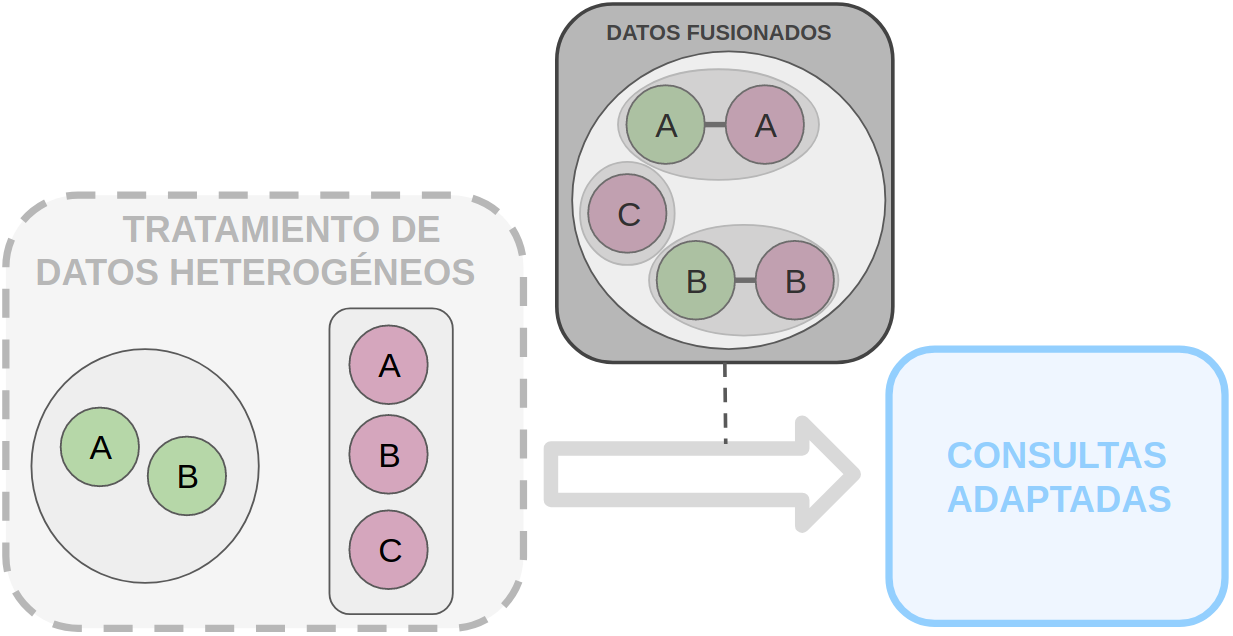
\includegraphics[width=1.0\textwidth]{imagenes/arquitectura/datos-agregados.png}
    \caption{Consulta sobre los datos fusionados}
    \label{fig:datos-agregados}
\end{figure}


Centrándonos en nuestro problema de adaptación de dietas, se utilizan dos fuentes de datos: una primera formada por recetas, y una segunda base de datos con información nutricional, ambas detalladas en el apartado \ref{sec:bd_recetas}. Al conectar las recetas con la base de datos nutricional (a través de sus ingredientes), podremos extrapolar dicha información y obtener las características nutricionales de las recetas (ver Figura \ref{fig:mapping-entre-recetas-1}). De esta forma, se podrá comprobar si los ingredientes cumplen o no las restricciones impuestas (y en su caso, modificarlos por otros más adecuados). Es en este punto es donde toma relevancia el tratamiento de datos heterogéneos, que nos permite obtener información especializada que no viene incluida en los datos de las recetas. 


\begin{figure}[H]
    \centering
    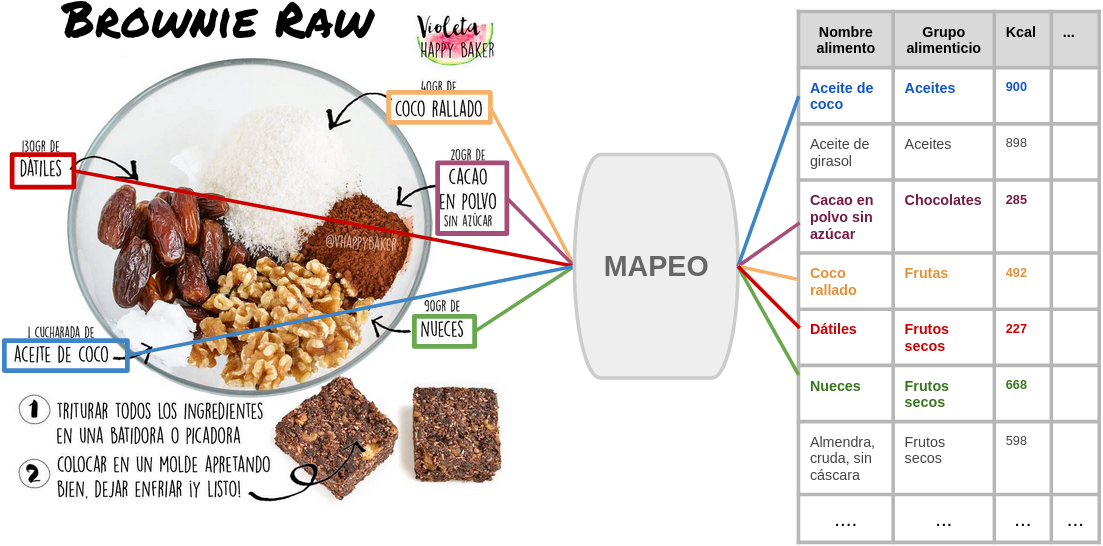
\includegraphics[width=1.0\textwidth]{imagenes/app/MAPEO ENTRE DATOS.png}
    \caption{Mapeo de datos de fuentes heterogéneas}
    \label{fig:mapping-entre-recetas-1}
\end{figure}


\section{Aplicación móvil}
Para ilustrar cómo funciona la solución diseñada para el problema de adaptación de recetas, se ha diseñado un prototipo funcional de aplicación móvil que permita ver su comportamiento de una forma más cómoda y realista, coherente a la línea que se sigue hoy en día con este tipo de pseudo-recomendaciones.


\subsection{Arquitectura}

En la Figura \ref{fig:arquitectura-app} se muestra la arquitectura global de la aplicación de adaptación de recetas. A través de la interfaz móvil, se realizan consultas al sistema de adaptación de recetas realizando consultas a la API, para obtener recetas adecuadas a las restricciones. A su vez, se hace uso de una base de datos de recetas, también accesible desde la API.

\begin{figure}[H]
    \centering
    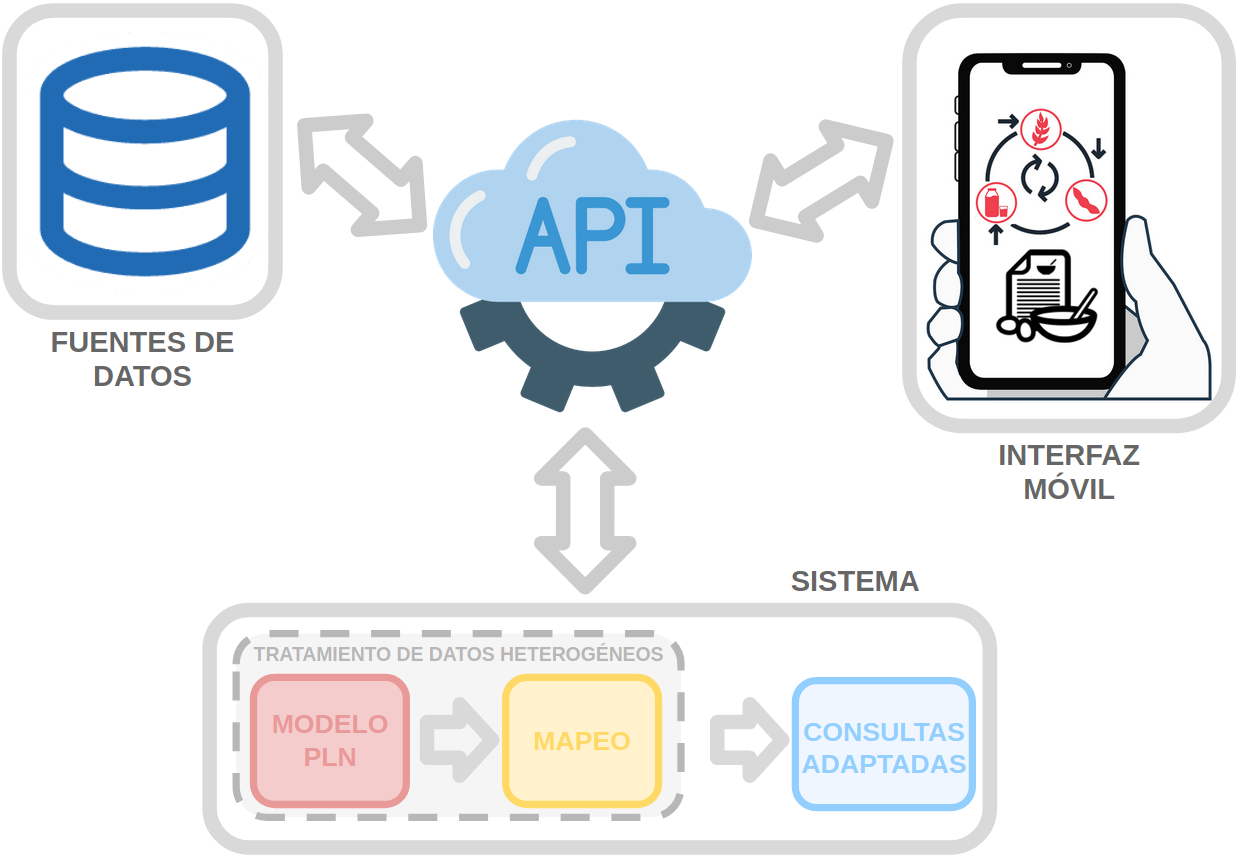
\includegraphics[width=1.0\textwidth]{imagenes/app/arq.png}
    \caption{Arquitectura de la aplicación}
    \label{fig:arquitectura-app}
\end{figure}

\subsection{Tecnologías utilizadas}

A continuación se enumeran las tecnologías utilizadas para la implementación y puesta en funcionamiento del sistema descrito.

\begin{enumerate}
    \item Para la Interfaz de Programación de Aplicaciones (API) se ha utilizado el lenguaje de programación Python con la librería Flask (\url{https://flask.palletsprojects.com/en/1.1.x/}).
    
    \item Para la base de datos se ha utilizado MongoDB (\url{www.mongodb.com/es}), un sistema de base de datos no estructuradas, orientado a colecciones de documentos. 
    
    \item Para la implementación de la aplicación, se ha utilizado IONIC  (\url{https://ionicframework.com/}), un kit de desarrollo Software de código abierto, el cual permite la creación de aplicaciones a nivel web y móvil (tanto para el sistema operativo Android como iOS). 
    
\end{enumerate}


\subsection{Fuentes de datos}\label{sec:bd_recetas}
Para el funcionamiento correcto del módulo, es necesario utilizar una base de datos que permita gestionar las recetas así como una base de datos de composición alimenticia para obtener la información nutricional de los alimentos.

\subsubsection{Base de datos de recetas}
En nuestro caso, hemos utilizado recetas procedentes de una colección de Food.com\footnote{\url{www.food.com}} proporcionada por Kaggle. Esta colección se llama  \textit{Food.com Recipes and Interactions}, que tal y como indica su nombre, está orientada al estudio de recetas e interacciones entre usuarios\footnote{\url{www.kaggle.com/shuyangli94/food-com-recipes-and-user-interactions}}. Puesto que no necesitamos las interacciones de los usuarios, únicamente hemos importado el fichero correspondiente a las recetas sin preprocesar (RAW\_recipes.csv\footnote{\url{www.kaggle.com/shuyangli94/food-com-recipes-and-user-interactions\#RAW\_recipes.csv}}).

La elección de este conjunto de datos viene dada por el origen de las recetas que lo forman. Esta colección no contiene ninguna receta procedente de las páginas web de las que se obtiene el conjunto de recetas del corpus con el que se entrena el modelo de Word Embedding. De esta forma, aseguramos que nuestros resultados con este módulo son válidos y no están sesgados por las recetas que utilizamos, pues no se han empleado para la construcción del modelo del lenguaje. Además, el contenido de dichas recetas está en inglés (recordemos que el modelo de lenguaje implementado está en dicho idioma) e incluyen todos los atributos de recetas requeridos por el módulo.

Para gestionar la base de datos de recetas, hemos utilizado tres colecciones de datos:
\begin{itemize}
    \item \textbf{Colección de recetas originales}: esta colección almacena todas las recetas utilizadas para el sistema de adaptación de recetas. Antes de insertar las recetas en la base de datos, hemos prescindido de aquellas columnas del conjunto de Kaggle que no nos aportan información útil, quedándonos únicamente con aquellas que sí nos interesa utilizar en el Módulo de Consultas Adaptadas. Asimismo, hemos añadido un campo \textit{Imagen}, para mejorar la visualización en el prototipo. En la Tabla \ref{table:ejemplo_receta} se muestra el contenido de las recetas de esta colección.
    
    \item \textbf{Colección de recetas adaptadas}: esta colección almacena recetas ya adaptadas a una restricción mediante el Módulo de Consultas Adaptadas. Contiene la misma estructura de atributos detallada en la sección anterior (ver Tabla \ref{table:ejemplo_receta}), con dos diferencias: en primer lugar, añade un atributo para almacenar la restricción aplicada sobre la receta y, en segundo lugar, los atributos \textit{Ingredientes} y \textit{Pasos en la aplicación} contienen dos nuevos campos, que almacenan si existe una modificación y, en caso afirmativo, de cuál se trata.
    
    \item \textbf{Colección de etiquetas de recetas}: una de las ventajas del conjunto de datos utilizado es que las recetas contienen un campo \textit{Etiquetas} que permite realizar clasificaciones sobre ellas. En nuestro caso, hemos definido una colección de etiquetas con algunas de las utilizadas en las recetas con el fin de poder clasificarlas en base a las etiquetas que nos sean de utilidad y realizar consultas por medio de ellas. Esta colección contiene la etiqueta, con un nombre e imagen añadida por nosotros para mejorar la de visualización en el prototipo.
    
\end{itemize}

\setlength{\tabcolsep}{2pt} 
\begin{table}[H]
\begin{tabular}{p{0.17\textwidth}|p{0.5\textwidth}|p{0.27\textwidth}}
\textbf{Atributo} & \textbf{Contenido} & \textbf{Tipo} \\ \hline 
Descripción & Descripción de la receta, consejos y algunos comentarios extra & cadena de caracteres \\
% Identificador de receta & Identificador de la receta en la colección & cadena de caracteres \\
Imagen & Imagen de la receta & cadena de caracteres \\
Nombre & Nombre de la receta & cadena de caracteres \\
Ingredientes & Lista de ingredientes de la receta & lista de cadena de caracteres \\
Minutos & Tiempo de preparación de la receta en minutos & cadena de caracteres \\
% n\_ingredients & Número de ingredientes en la receta & número entero \\
% n\_steps & Número de pasos en la preparación de la receta & número entero \\
Nutrientes & Lista con los valores nutricionales de la receta en el siguiente orden: kilocalorías, grasas totales, azúcar, sodio, proteína, grasas saturadas y carbohidratos & lista de números de coma flotante \\
Pasos en la preparación & Lista con los pasos para preparar la receta & lista de cadenas de caracteres \\
Etiquetas & Lista de etiquetas asociada a la receta (p.ej., ``30 minutes or less'') & lista de cadenas de caracteres
\end{tabular}
\caption{\label{table:ejemplo_receta} Descripción de los campos en la colección de recetas originales}
\end{table}


\subsubsection{Base de datos de Composición de Alimentos}

Como se ha comentado previamente, este módulo requiere un procedimiento previo de tratamiento de datos heterogéneos de las recetas con una base de datos de composición de alimentos para obtener información nutricional de los ingredientes que forman las recetas. En este módulo se ha utilizado la Base de Datos de Composición de Alimentos i-Diet~\cite{iDietrf}, que se encuentra detallada en el Capítulo \ref{ch:Pruebas} (Apartado \ref{subsec:idiet}). 

La elección de i-Diet se debe principalmente a dos de sus características principales. Por un lado se trata de una base de datos de alimentos muy depurada que además de ser utilizada por nutricionistas, se emplea en sistemas informáticos de nutrición y dietética~\cite{iDietrf}. Por otro lado, está orientada a su uso conjunto con platos (lo cual es difícil de encontrar en este ámbito), por lo que contiene una cantidad representativa de ingredientes que suelen aparecer en recetas de cocina.


\subsection{Sistema para Adaptación de Recetas}

Para poder llevar a cabo la adaptación de las recetas en base a una restricción alimenticia dada se siguen los siguientes pasos:
\begin{enumerate}
    \item En primer lugar, se debe seleccionar una receta junto con la restricción alimenticia a aplicar, los cuales son los datos de entrada al sistema. En nuestro caso, esta receta se selecciona de entre una lista proporcionada. De esta receta, obtenemos sus ingredientes, de los cuales obtenemos sus correspondientes representaciones vectoriales con el Módulo de Procesamiento de Lenguaje Natural. 
    
    \item Una vez tenemos las representaciones vectoriales de los ingredientes se realiza un mapeo de estos alimentos hacia la base de datos de composición nutricional, para obtener información específica de cada uno de dichos alimentos. Este paso se lleva a cabo en el Módulo de Mapeo.
    
    \item Con toda la información de los ingredientes ya disponible, realizamos una consulta para ver cuales de ellos cumplen con las restricciones alimenticias proporcionadas (actualmente, el sistema incorpora dos restricciones a elegir: dieta vegana y dieta vegetariana). Para cada alimento que no la cumpla, se vuelve a recurrir al módulo de mapeo, para recomendar un posible alimento que pueda sustituirlo. En este paso, al usar las representaciones capaces de capturar la información semántica de los ingredientes, se posibilita que la opción proporcionada se adapte a dicha receta, puesto que este segundo mapeo se realiza únicamente sobre los elementos permitidos devolviendo el más cercano al ingrediente a modificar. Finalmente, se proporciona como la salida, la receta con los cambios correspondientes. En nuestro caso, en vez de proporcionar una única alternativa, hemos decidido facilitar varias opciones de reemplazo para cada ingrediente incompatible. Con ello, se da la posibilidad de elegir entre uno de ellos o realizar alguna modificación previa a la adaptación final de la receta. 
\end{enumerate}


\subsection{Interfaz de Programación de Aplicaciones (API)}

La Interfaz de Programación de Aplicaciones permite acceder a través de peticiones a las operaciones CRUD sobre las recetas, además de conectarse al sistema de adaptación de recetas y poder realizar las adaptaciones que se requieran (ver Figura \ref{fig:arquitectura-app}). 

\subsubsection{Operaciones CRUD}

Se ha realizado el diseño e implementación de una API REST completamente funcional, que se conecta a las colecciones de la base de datos para realizar operaciones sobre los datos almacenados. Para ello, se han definido rutas con todas las consultas necesarias para el funcionamiento de la aplicación tanto a nivel de receta como de colección: lista completa de recetas, recetas que incluyan alguna etiqueta concreta, etc. Para poder realizar peticiones a nivel de receta, se ha llevado a cabo el diseño del correspondiente modelo de datos de Receta, para describir el objeto Receta y poder trabajar con la estructura de los datos en las colecciones de recetas. Este objeto Receta se utiliza para llevar a cabo las operaciones CRUD correspondientes para crear, leer, actualizar y eliminar recetas de la base de datos.


\subsubsection{Adaptación de recetas}

Se han implementado las rutas necesarias para poder realizar peticiones al Sistema de Adaptación de recetas, y así obtener recetas adaptadas acorde a alguna restricción concreta. Para ello, a través de la API se cargan los modelos predictivos necesarios para poder llevar a cabo dichas acciones.

\subsection{Aplicación}

\subsubsection{Diseño conceptual}

Previa a la implementación del prototipo que se utiliza en esta aplicación, se ha llevado a cabo el diseño conceptual de la aplicación. En primer lugar, las capacidades de la aplicación se pueden ver en el diagrama de casos que se ha obtenido para esta aplicación (ver Figura \ref{fig:diagrama_casos}). Si nos centramos en la arquitectura de la información, se han descrito las tareas usando un diagrama de tareas HTA (ver Figura \ref{fig:diagramahta}). Los posibles planes para el diagrama HTA se enumeran a continuación:
\begin{enumerate}
    \item \textbf{Plan 0}: Si sólo quiere consultar recetas
    \begin{enumerate}
        \item Hacer 1-2-3-4-5-6-8 (7 opcional)
    \end{enumerate}
    \item \textbf{Plan 1}: Si quiere adaptar recetas
        \begin{enumerate}
        \item Hacer 1-2-3-4-5-6-8 (7 opcional)
        \item Si quiere guardar la receta hacer 6.3
    \end{enumerate}
\end{enumerate}


El contenido de la información se ha descrito mediante un diagrama de conceptos (ver Figura \ref{fig:diagrama_conceptual}), en el que se puede apreciar las relaciones existentes entre las recetas (originales y adaptadas) y el usuario en cuestión. Por último, se han descrito los mapas de flujo para el usuario de la aplicación móvil a través de un diagrama WireFlow que se puede ver en la Figura \ref{fig:diagrama_wireflow}.

En base a estos diagramas, se puede apreciar que la funcionalidad implementada en la aplicación se corresponde con una tarea: la adaptación de recetas. Por ello, queremos resaltar que estos diagramas (y por tanto, la aplicación) podrían integrarse en el diseño de una aplicación móvil de dietética más general, en la que entre otras muchas tareas, una de las facilitadas fuera la adaptación en base a restricciones del usuario.


\begin{figure}[H]
    \centering
    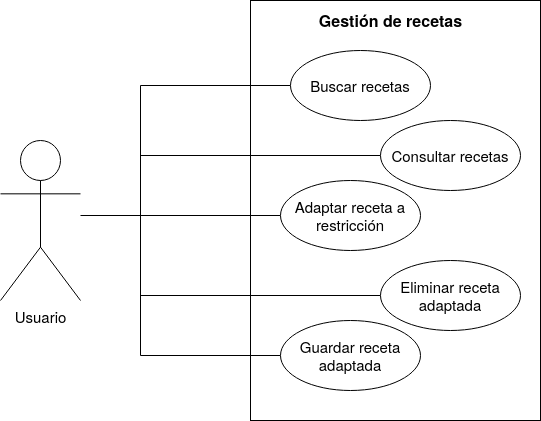
\includegraphics[width=0.6\textwidth]{imagenes/app/diagramas/Casos de uso.png}
    \caption{Diagrama de casos de uso de la aplicación}
    \label{fig:diagrama_casos}
\end{figure}


\begin{figure}[H]
    \centering
    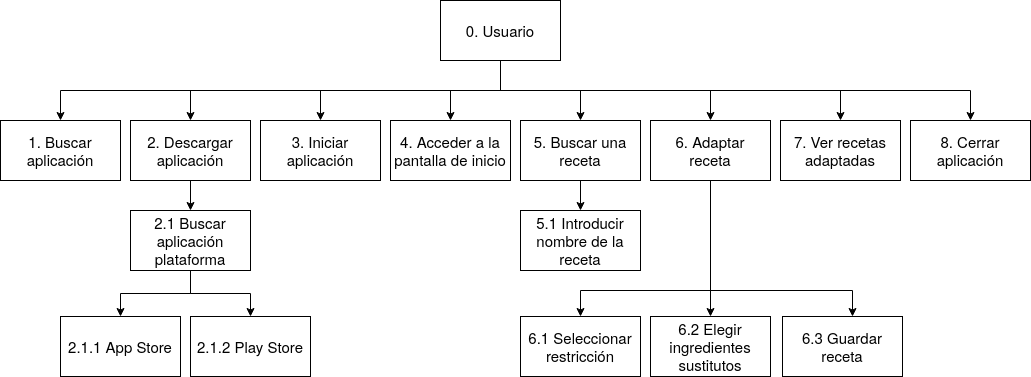
\includegraphics[width=1.0\textwidth]{imagenes/app/diagramas/diagrama-hta.png}
    \caption{Diagrama HTA de la aplicación}
    \label{fig:diagramahta}
\end{figure}



\begin{figure}[H]
    \centering
    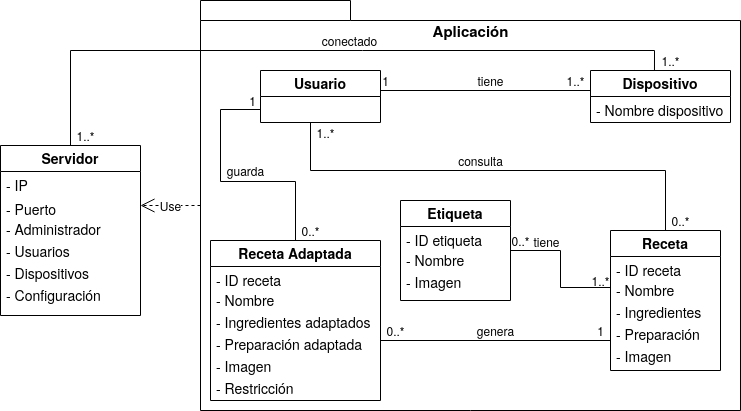
\includegraphics[width=1.0\textwidth]{imagenes/app/diagramas/diagrama_conceptual.png}
    \caption{Diagrama Conceptual de la aplicación}
    \label{fig:diagrama_conceptual}
\end{figure}


\begin{figure}[H]
    \centering
    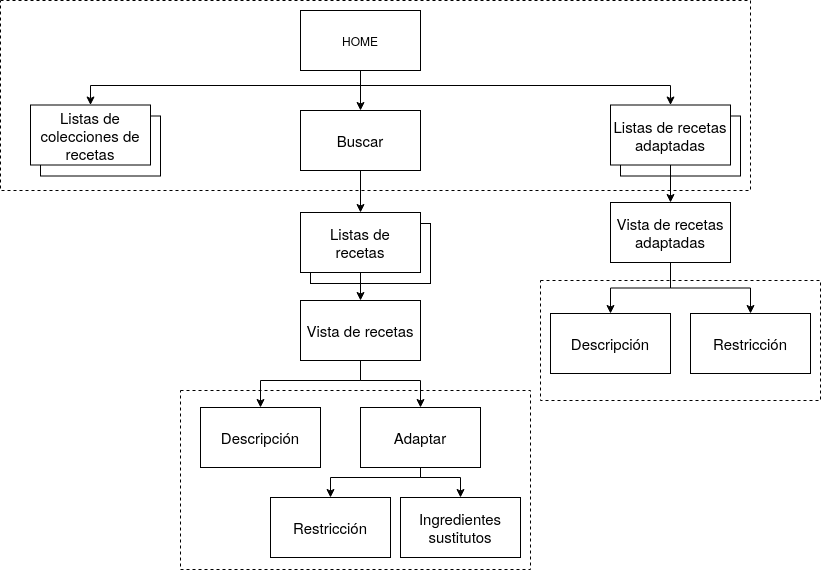
\includegraphics[width=1.0\textwidth]{imagenes/app/diagramas/Wireflow.png}
    \caption{Diagrama Wireflow de la aplicación}
    \label{fig:diagrama_wireflow}
\end{figure}

\subsubsection{Funcionamiento de la aplicación}
En la selección de Figuras \ref{fig:ejemplo_uso} se puede ver el comportamiento básico de la aplicación, el cual consiste en acceder a una receta y obtener su versión adaptada. Tal y como se puede ver, a partir de la navegación por colecciones de recetas (Figura \ref{fig:pantallas_basicas_1}), se puede acceder a una receta específica (Figura \ref{fig:pantallas_basicas_2}) y obtener una adaptación de la misma (Figura \ref{fig:pantallas_basicas_3}). Estas tres pantallas de la aplicación tan sólo forman una versión simplificada del funcionamiento de la aplicación. En el Apéndice \ref{ch:Anexo_Pantallas} se puede ver de forma detallada toda la estructura de navegación en esta aplicación a través de los flujos de datos entre las distintas pantallas implementadas. 

\begin{figure}[H]
    \centering
    
    \begin{subfigure}[b]{0.322\linewidth}
        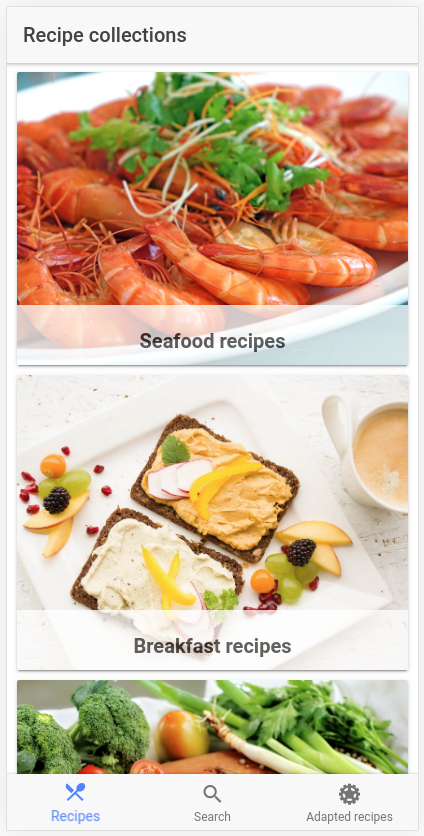
\includegraphics[width=\linewidth]{imagenes/app/pantallas/app_1.png}
        \caption{Colecciones}
        \label{fig:pantallas_basicas_1}
    \end{subfigure}
    \begin{subfigure}[b]{0.32\linewidth}
        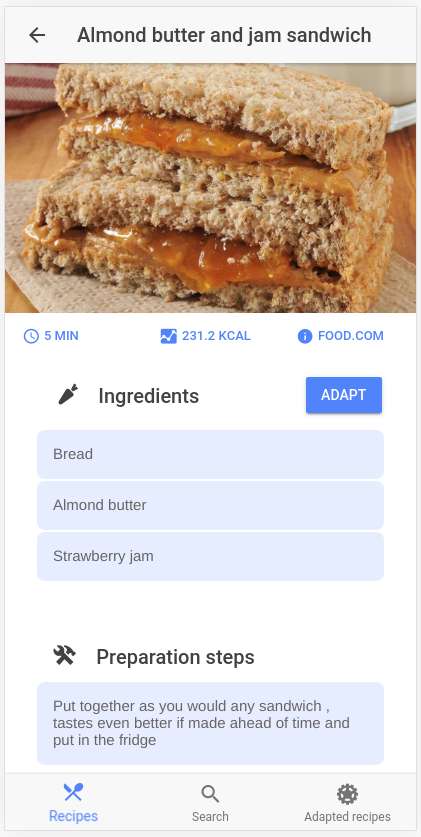
\includegraphics[width=\linewidth]{imagenes/app/pantallas/app_2.png}
        \caption{Receta original}
        \label{fig:pantallas_basicas_2}
    \end{subfigure}
    \begin{subfigure}[b]{0.32\linewidth}
        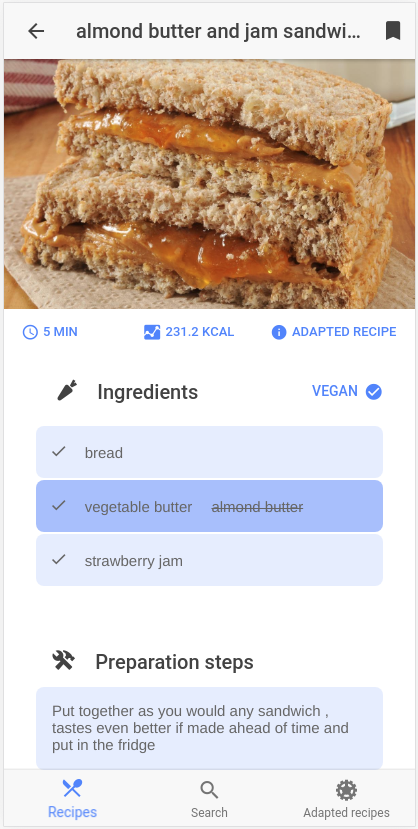
\includegraphics[width=\linewidth]{imagenes/app/pantallas/app_3.png}
        \caption{Receta adaptada}
        \label{fig:pantallas_basicas_3}
    \end{subfigure}
    \caption{Pantallas de la aplicación: funcionamiento básico}
    \label{fig:ejemplo_uso}
\end{figure} 

\subsection{Siguientes pasos en el desarrollo de la aplicación móvil}

Tal y como se ha visto en la sección anterior, a pesar de que la funcionalidad básica está implementada, aún queda un amplio recorrido para obtener una versión final de la interfaz gráfica de esta aplicación móvil, ya que, tal y como se ha descrito, se encuentra en una primera iteración del proceso de desarrollo. Con este prototipo pretendemos centrarnos en la funcionalidad, no sólo con el objetivo de ver el funcionamiento de la inteligencia por debajo de la aplicación, sino también para ver las posibilidades que tienen los sistemas adaptados tal como el que se ha implementado en este trabajo. 

Para continuar con el diseño de la interfaz, los pasos a seguir parten de la evaluación de la aplicación con y sin usuarios: en primer lugar una evaluación general, con lista de chequeos y los consecuentes informes de evaluación heurística, seguidos del test de usabilidad de la aplicación y finalmente, un test de evaluación con usuarios para analizar el éxito y dificultades al interactuar con la aplicación. A través de estas evaluaciones, se podrán realizar las siguientes iteraciones, más centradas en el diseño y ultimación de las funcionalidades de la aplicación con lo que esperan los usuarios finales.



\chapter{Experimentación y resultados}
\label{ch:Pruebas}

\begin{quote}
  Este capítulo recoge la experimentación realizada en los tres módulos en los que se divide este trabajo, así como los resultados obtenidos y una breve discusión sobre los mismos.
\end{quote}


\section{Diseño experimental}
% Fuentes de datos
% Máquina utilizada
% He decidido hacerlo por módulos

% Explicar validación y que únicamente tiene presencia en tal parte. --> ¿Cómo se han organizado los expermientos?

Para llevar a cabo la experimentación del sistema que se ha desarrollado se ha optado por analizar el funcionamiento de cada uno de los módulos del sistema de manera independiente. Todos los experimentos realizados se han ejecutado de forma local, utilizando para ello mi ordenador personal. La organización de los experimentos se han llevado a cabo de la siguiente forma:

\begin{enumerate}
    \item Para estudiar los resultados obtenidos con el modelo de lenguaje (Sección \ref{sec:res_pln} de este capítulo), se ha decidido llevarlo a cabo desde el punto de vista de la visualización de las representaciones generadas con el modelo de Word Embedding. Para ello, se ha decidido representar las relaciones entre las palabras mediante la obtención de aquellas que son más similares a una dada en el vocabulario. Esta decisión se ha tomado debido a la dificultad de analizar las representaciones originales por la alta dimensionalidad de las mismas. Para ello, se ha experimentado con visualizaciones del vocabulario del modelo. Con la ayuda de estas experimentaciones, hemos ajustado los parámetros de entrenamiento del modelo para optimizar su funcionamiento. El modelo final ha sido entrenado durante 30 épocas con vectores de dimensión 300 con las palabras que aparecen 3 o más veces en el corpus de entrenamiento, Para el contexto de cada palabra se ha fijado el tamaño de ventana a 5. Finalmente, el modelo obtenido tiene un vocabulario de 11,288 palabras.
    
    \item Para la experimentación con el módulo de Mapeo (Sección \ref{sec:res_mapeo}), se ha realizado una validación de las medidas de distancia implementadas para determinar cuál es la más efectiva en nuestro problema, y que por tanto, usaremos en nuestra solución. Concretamente, buscaremos las correspondencias de los elementos en la base de datos de i-Diet~\cite{iDietrf} con los elementos en USDA~\cite{gebhardt2008usda} (ya introducida en el Capítulo \ref{ch:Capitulo 3}). Ambas bases de datos, se utilizan en el proyecto Stance4Health\footnote{Stance4Health (Smart Technologies for Personalised Nutrition and Consumer Engagement) es un proyecto financiado por la Unión Europea por el programa de investigación e innovación Horizon 2020. Más información: \url{https://www.stance4health.com}.}, donde tiene cabida esta tarea de mapeo (más información se puede encontrar en~\cite{morales2020word}). Stance4Health, tiene como objetivo desarrollar un servicio de nutrición personalizado para optimizar la actividad de la microbiota intestinal, haciendo uso para ello de múltiples bases de datos de composición nutricional de distinta procedencia, entre las que se encuentran \textit{i-Diet} y \textit{USDA}, ambas explicadas con mayor detalle en la Sección \ref{sec:bds}. Los mapeos obtenidos han sido contrastados con las correspondencias reales para obtener el porcentaje de acierto de cada una de las medidas de distancia. La decisión de qué medida es la más adecuada para el sistema se ha tomado en función del porcentaje de aciertos obtenido con cada una de ellas.
    
    \item Por último, los experimentos realizados con la aplicación de adaptación de recetas (Sección \ref{sec:res_adap}) se han orientado al estudio del comportamiento de la inteligencia por debajo de la aplicación, llevada a cabo en el Módulo de Consultas Adaptadas. Para ello, se muestra de forma ejemplificada su comportamiento con resultados representativos que engloban su comportamiento general. Para este módulo no se requiere el uso de ninguna otra base de datos adicional a las utilizadas en el prototipo de la aplicación (explicadas en el Capítulo \ref{ch:Consultas_Adaptadas}).
    
\end{enumerate}


\subsection{Bases de datos utilizadas}\label{sec:bds}

\subsubsection{Base de datos de Composición Nutricional i-Diet}\label{subsec:idiet}
La base de datos i-Diet~\cite{iDietrf} es una base de datos de composición nutricional de origen español. Esta base de datos, está formada por un total de 734 alimentos y consta de 75 atributos, entre los que se encuentra su descripción en español y en inglés, grupo alimenticio y los valores correspondientes de macronutrientes y micronutrientes.

\setlength{\tabcolsep}{3pt} 
\begin{table}[H]
	\begin{center}
		\begin{tabular}{p{0.06\textwidth}|p{0.18\textwidth}|p{0.18\textwidth}|p{0.38\textwidth}|p{0.03\textwidth}}
			\rule{0pt}{12pt}
			\textbf{ID}  & \textbf{Descripción (ESP)} & \textbf{Descripción (ENG)} & \textbf{Grupo alimenticio} & ... \tabularnewline
			\hline
			
			96 & Cebolla & Onion &  HORTALIZAS BULBOSAS & ... \\
			290 & Manzana & Apple & FRUTAS  & ... \\			
		
		\end{tabular}
		{\caption{Algunos ejemplos de la base de datos i-Diet} \label{table5}}
	\end{center}
\end{table}

En la Tabla \ref{table5} se puede ver la estructura simplificada de esta base de datos, con dos ejemplos de alimentos contenidos en ella. En nuestro caso, para los mapeos utilizaremos la columna ``\textit{Descripción ENG}'', la cual contiene la descripción en inglés de cada alimento almacenado en la base de datos (recordemos que el modelo de lenguaje está dicho idioma).


\subsubsection{Base de datos de Composición Nutricional USDA}

La base de datos de Alimentos y Nutrientes para Estudios Dietéticos (FNDDS) del Departamento de Agricultura de los Estados Unidos (USDA)\footnote{\url{https://data.nal.usda.gov/dataset/food-and-nutrient-database-dietary-studies-fndds}}, es una base de datos de composición nutricional de referencia, creada con el objetivo de obtener los valores nutricionales a partir de las cantidades de alimentos consumidos en Estados Unidos. Esta base  de datos esta formada por distintas tablas; alimentos y bebidas, nutrientes, ingredientes, valores nutricionales de ingredientes y porciones y unidades de medida de alimentos. En concreto, en este trabajo hemos utilizado únicamente una de las tablas contenidas en esta base de datos: \textit{Nutrient Values}, la cual nos permite acceder a los datos nutricionales de una gran cantidad de alimentos consumidos en Estados Unidos. Esta tabla está formada por 8690 elementos de los que se tienen 69 atributos con la descripción en inglés, el código de la categoría de alimentos, macronutrientes y micronutrientes. En la Tabla \ref{table6} se muestran dos ejemplos de esta base de datos, con una estructura simplificada de la misma. 


\setlength{\tabcolsep}{2pt}
\begin{table}[H]
	\begin{center}
		% \begin{tabular}{lllll}
		\begin{tabular}{p{0.17\textwidth}|p{0.29\textwidth}|p{0.16\textwidth}|p{0.19\textwidth}|p{0.03\textwidth}}
			
			\rule{0pt}{12pt}
			\textbf{Código del alimento} & \textbf{Descripción \newline alimenticia \newline principal} & \textbf{Código de\newline categoría WWEIA}& \textbf{Descripción de categoría WWEIA} & ... \tabularnewline
			\hline
			
			% \quad 11320000 & Soy milk & 1404 & Milk substitutes & ... \\
			\quad 75117020 & Onions, mature, raw & 6414 & Onions & ... \\
			\quad 63101210 & Apple, cooked or canned, with syrup & 6002 & Apples & ... \\
% 			\quad 63101310 & Apple, baked, NS as to added sweetener & 6002 &Apples & ...\\
			
			% \quad 74601000 & Tomato    soup, NFS & 3802 & Soups & ... \\			
			
		\end{tabular}
	\end{center}
	{\caption{Algunos ejemplos de la base de datos USDA} \label{table6}}
\end{table}


% Añadir estructura de las tblas que están en el ipmu

% informacion detallada de las bases de datos.

% descripción y un par de ejemplos. 
% atributos
% cantidad de atributos
% cantidad de tuplas



\section{Resultados y discusión}

\subsection[Resultados del Módulo de PLN]{Resultados del Módulo de Procesamiento de Lenguaje Natural}\label{sec:res_pln}

A priori, comprender el comportamiento de un modelo de Word Embedding puede resultar complejo, debido a la alta dimensionalidad de los vectores númericos que se obtienen de las palabras con las se trabaja. Por ello, se ha optado por utilizar el algoritmo de Aprendizaje Automático t-SNE (\textit{t-Distributed Stochastic Neighbor Embedding}) para obtener visualizaciones de dichas representaciones de palabras. Con este algoritmo, se obtiene una representación bidimensional de dichos vectores, favoreciendo que aquellos que sean más similares aparezcan más cercanos en el plano, y aquellos más diferentes queden espacialmente más alejados entre ellos. De esta forma, podremos interpretar los resultados obtenidos con dicho modelo, así como analizar las posibles relaciones que puedan existir entre el conjunto de palabras contenidas en el vocabulario resultante del entrenamiento del modelo.

\begin{figure}[H]
    \centering
    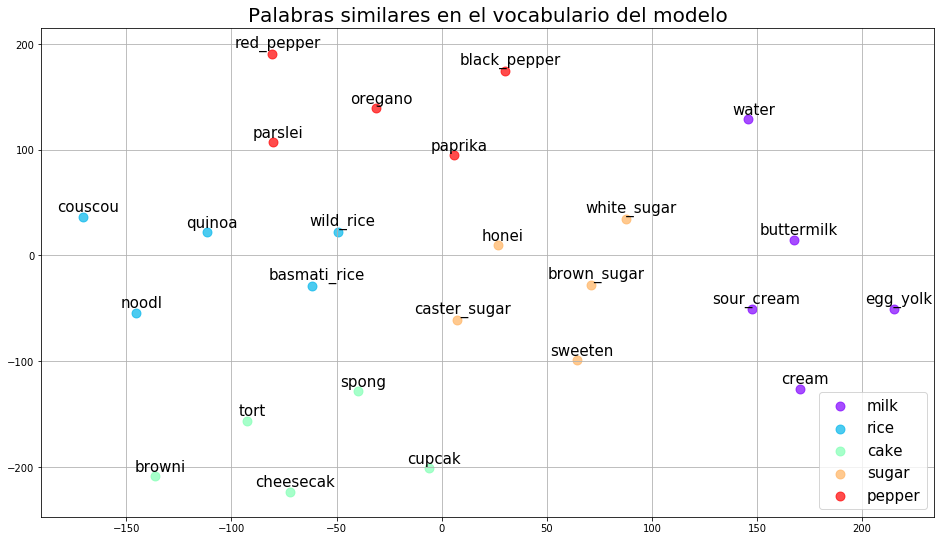
\includegraphics[width=1.0\textwidth]{imagenes/resultados/word-embedding-2.png}
    \caption{Visualización del modelo: elementos similares (ejemplo 1)}
    \label{fig:wordembedding_vis1}
\end{figure} 

En nuestro caso, para analizar la calidad de las representaciones que obtenemos con el modelo de procesamiento de lenguaje vamos a visualizar posibles relaciones de similitud entre palabras del vocabulario del modelo con una de las principales aplicaciones de los modelos de Word Embedding: detectar elementos similares dentro del vocabulario. Esta funcionalidad viene implementada dentro de la librería de Procesamiento de Lenguaje Natural que utilizamos para el entrenamiento y utilización del modelo (\textit{Topic Modelling  Gensim}\footnote{\url{https://radimrehurek.com/gensim/}}). De esta forma, para una palabra dada, podremos obtener aquellas más similares que se encuentren representadas dentro del vocabulario del modelo de lenguaje.

En la Figura \ref{fig:wordembedding_vis1} se pueden ver, para los alimentos \textit{leche}, \textit{arroz}, \textit{tarta}, \textit{azúcar} y \textit{pimiento}, las palabras del vocabulario del modelo más similares para dichos elementos. Como se puede observar, dichas palabras se muestran en inglés tras el proceso de lematización aplicado al conjunto de entrenamiento para la creación del modelo (tal y como se explica en el Capítulo \ref{ch:Capitulo 5}). En dicha figura se muestra cómo, por ejemplo, los elementos más similares a \textit{azúcar} son azúcar moreno, azúcar blanco, endulzar, etc; o cómo para \textit{arroz}, el modelo devuelve \textit{arroz salvaje}, \textit{arroz basmati}, \textit{quinoa} o \textit{couscous}. En este último ejemplo se aprecia la gran potencia que aportan estos modelos, donde detecta que el \textit{couscous} es similar al arroz, llegando a ese punto únicamente a través del modelo predictivo entrenado con las recetas. Con este caso se demuestra cómo el modelo entrenado ha sido capaz de capturar la semántica de los datos con los que se ha entrenado, bajo la idea de que alimentos utilizados en contextos y forma similares, guardan también una relación de parecido. Además, debido a su gran valor en cuanto a similitud, incluso podría ser un sustitutivo del mismo, ya que el uso, preparación, cocinado y combinación con otros ingredientes en recetas es similar entre uno y otro. 

\begin{figure}[H]
    \centering
    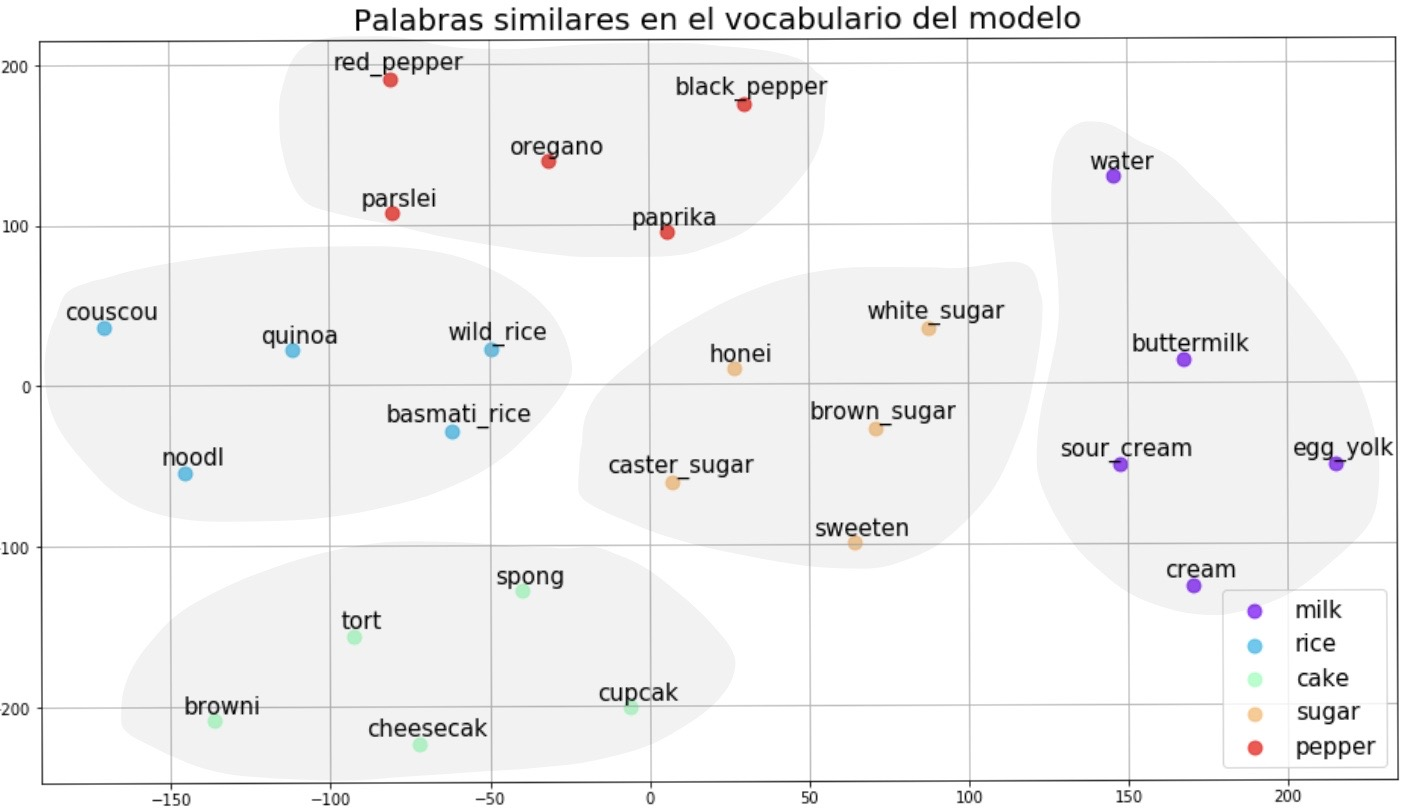
\includegraphics[width=1.0\textwidth]{imagenes/resultados/word-embedding-3.jpg}
    \caption{Visualización del modelo: localización espacial de los items (ej.1)}
    \label{fig:wordembedding_vis2}
\end{figure}


Por otra parte, si en la Figura \ref{fig:wordembedding_vis1} nos fijamos en el vocabulario más similar obtenido para \textit{Leche}, se puede ver cómo se han obtenido como similares \textit{yema de huevo} y \textit{mantequilla}. Esto se puede deber a que gran parte de las recetas que incluyan el ingrediente \textit{leche} sean postres, y aparezca acompañado o con un uso similar a los últimos mencionados. Por ello, es importante hacer ver que las representaciones obtenidas pueden estar sesgadas por las características de las recetas que se utilicen. Aquí se hace necesario utilizar grandes conjuntos de recetas, que permitan abarcar una gran cantidad de combinaciones de ingredientes, así como preparaciones de los mismos, para que el resultado sea lo más realista posible. En este caso, sí podemos concluir que se ha obtenido una buena representación, ya que otro de los elementos más similares es \textit{agua}, lo cual nos permite ver que se están teniendo en cuenta otras características en su representación interna (como en este caso, que es similar a otros elementos del vocabulario que también son bebidas). Además, en dicha imagen se puede ver cómo los elementos similares a cada una de las descripciones textuales elegidas (nombres de alimentos) se encuentran cercanas en cuanto a su representación espacial. Este hecho se aprecia de forma más clara en la Figura \ref{fig:wordembedding_vis2}, donde se han delimitado sobre la imagen aquellos elementos más similares a cada uno de los escogidos.


\begin{figure}[H]
    \centering
    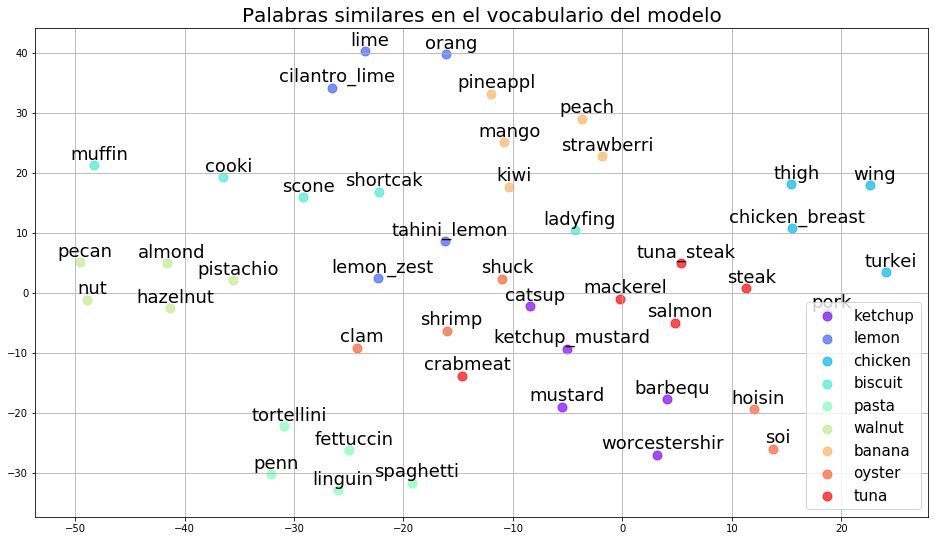
\includegraphics[width=1.0\textwidth]{imagenes/resultados/word-embedding-4.png}
    \caption{Visualización del modelo  (ejemplo 2)}
    \label{fig:wordembedding_vis3}
\end{figure}


Si obtenemos una visualización con mayor número de alimentos, vemos que al aumentar la cantidad de elementos en la visualización no es tan sencillo encontrar una ``separación espacial'' tan clara como la de la Figura \ref{fig:wordembedding_vis2}. Esto se debe a que estamos en un contexto en el que un ingrediente puede tener múltiples usos y en gran cantidad de contextos distintos (p.ej, el limón se utiliza en postres pero también en pescados o carnes). Este hecho se aprecia en la Figura \ref{fig:wordembedding_vis3}. En esta figura podemos contrastar cómo de nuevo, alimentos con usos muy similares son detectados por el modelo sin necesidad de ser el mismo alimento o derivado del mismo: pollo y pavo (a la derecha en azul en la figura) o atún y salmón (en rojo a la derecha), son ejemplos de ello.

Otro caso relevante en el que la semántica de los alimentos ha sido tenida en cuenta dentro del modelo se aprecia en en los elementos similares obtenidos para \textit{Limón} y para \textit{Plátano}. Podemos ver que a pesar de que ambos, \textit{Limón} y \textit{Plátano}, son tipos de frutas, el modelo no se ha limitado a proporcionar como similares otras frutas, sino que en el caso del limón, ha sido capaz de representar características relacionadas con sabores: en este caso, todos los elementos más similares a \textit{Limón} también son cítricos, mientras que en los más parecidos a \textit{Plátano}, no hay ninguno con componente cítrico.

Con estos ejemplos, hemos podido comprobar la calidad de las representaciones obtenidas, puesto que capturan de forma precisa las semejanzas semánticas y sintácticas entre los alimentos, llegando incluso a ser capaz de representar sabores debido a las relaciones intrínsecas entre los alimentos. Estas relaciones se obtienen gracias al conjunto de entrenamiento utilizado que, al ser de instrucciones de preparación de recetas, permiten capturar información del contexto en el que se utilizan dichos alimentos, con cuáles se combinan y qué tipo de preparación y técnicas de cocinado se utilizan en ellos. Además, capturar la semántica de los alimentos en la representación del modelo de lenguaje teniendo en cuenta el uso de los mismos en el ámbito culinario no sólo permite detectar equivalentes, sino que abre una vía hacia la generación, alteración y adecuación de recetas teniendo en cuenta múltiples casuísticas.



\subsection{Resultados del Módulo de Mapeo}\label{sec:res_mapeo}

Tal y como se detalla en el Capítulo \ref{ch:Capitulo 6}, para analizar el funcionamiento de las distintas métricas de distancia utilizadas, se ha realizado un mapeo entre dos bases de datos nutricionales: i-Diet y USDA. Para cada elemento de i-Diet, se aplica el procedimiento de mapeo ya detallado para obtener su equivalente en USDA, utilizando las distintas medidas implementadas. En la Tabla \ref{table8} se pueden ver los resultados alcanzados con estas medidas de distancia. Para una mayor comprensión del modelo, hemos tenido en cuenta distintos niveles de cobertura de los resultados obtenidos. En la columna \textit{Top 1}, se muestra el porcentaje de elementos en la base de datos de i-Diet para los que se ha obtenido el mejor mapeo posible en la base de datos USDA. En el caso de la columna \textit{Top 2}, el valor obtenido se corresponde con el porcentaje de elementos en i-Diet cuyo mejor mapeo posible se encuentra entre los dos mejores resultados obtenidos con el procedimiento, y sucesivamente con el resto de columnas. En dicha tabla, se puede ver cómo las aproximaciones difusas nos permiten obtener los mejores resultados, superando las medidas de distancia semántica, sintáctica, o combinación de ambas. En concreto, la medida de \textit{Distancia difusa entre documentos} nos permite detectar mayor número de equivalencias. En los siguientes apartados se profundiza en los mapeos obtenidos con las distintas métricas para obtener una idea más concreta del comportamiento y eficacia de las mismas.



\setlength{\tabcolsep}{4pt} 
\begin{table}[H]
\small
\begin{tabular}{l|l|l|l|l|l}

\textbf{Medida de distancia} & \textbf{Top 1} &\textbf{Top 2}& \textbf{Top 3} & \textbf{Top 5} & \textbf{Top 10}\\ \hline
Distancia Jaccard & 16.75 & 20.16 & 22.20 & 25.20 & 27.52 \\
Word Mover's Distance & 30.65 & 35.55 & 36.92 & 40.87 & 44.82 \\ \hline
Distancia híbrida & 32.15 & 37.12 & 40.19 & 43.05 & 47.41 \\ \hline 
Distancia Jaccard difusa & 23.84 & 29.70 & 33.37 & 39.23 & 45.64 \\ 
Distancia entre documentos difusa & 35.55 & 40.46 & 43.46 & 47.00 & 53.26 \\ 
\end{tabular}
\caption{Resultados del mapeo ($\%$) con las medidas de distancia}\label{table8}
\end{table}



\subsubsection{Distancia sintáctica entre descripciones}

\begin{flushleft}
    \textit{Distancia de Jaccard}
\end{flushleft}
En la Tabla \ref{table:jaccard} se pueden ver algunos de los mapeos más representativos obtenidos con el procedimiento de mapeo usando la medida de distancia Jaccard. Como ya se ha introducido, esta medida de concordancia utiliza el conjunto de tokens preprocesados obtenidos a partir de cada una de las descripciones alimenticias para asignar un valor de distancia en función de los tokens que pertenecen al conjunto intersección.

\setlength{\tabcolsep}{2pt} 
\begin{table}[H]
\begin{tabular}{p{0.035\textwidth}p{0.24\textwidth}|p{0.26\textwidth}|p{0.27\textwidth}|p{0.10\textwidth}p{0.01\textwidth}}
& \textbf{Alimento a \newline mapear (i-Diet)} & \textbf{Alimento mapeado (USDA)} & \textbf{Mejor mapeo\newline posible (USDA)} & \textbf{Valor\newline distancia} &  \\ \hline

(1) & Peanut oil & Peanut oil & Peanut oil & 0.0 & \textcolor{myGreen}{\cmark} \\ 

(2) & Cauliflower & Cauliflower, raw & Cauliflower, raw & 0.199 & \textcolor{myGreen}{\cmark} \\

(3) & Anchovy &  Anchovy, canned &  Anchovy, canned & 0.125 & \textcolor{myGreen}{\cmark} \\

(4) & Chicory & Brioche & Chicory, beverage & 0.16 & \textcolor{myRed}{\xmark} \\

(5) & Avocado & Vodka & Avocado, raw & 0.33 & \textcolor{myRed}{\xmark} \\

(6) & Swett potatoes & Stewed potatoes & Sweet potato NFS & 0.0 & \textcolor{myRed}{\xmark} \\

\end{tabular}
\caption{\label{table:jaccard} Resultados obtenidos con la distancia de Jaccard}
\end{table}


Esta concordancia a nivel de cadena de caracteres se refleja en los resultados obtenidos, ya que en las tres primeras filas se obtienen mapeos adecuados debido al parecido sintáctico entre los elementos de ambas bases de datos (las descripciones son muy similares desde el punto de vista de caracteres utilizados). De igual forma, se puede apreciar de las filas (3) a (6), puesto que los resultados del mapeo no tienen ningún tipo de relación, más allá de la sintáctica, con los elementos mapeados (además de hacerlo con un valor de distancia mínimo, para nada representativo). A su vez, se puede ver en la fila (6) la falta de robustez con la que contamos con esta métrica, puesto que un mínimo error tipográfico en las descripciones lleva a un mapeo erróneo. 






% \setlength{\tabcolsep}{3pt} 
% \begin{table}[H]
% \begin{tabular}{p{0.045\textwidth}p{0.24\textwidth}|p{0.26\textwidth}|p{0.27\textwidth}|p{0.10\textwidth}p{0.01\textwidth}}
% & \textbf{Alimento a \newline mapear (i-Diet)} & \textbf{Alimento mapeado (USDA)} & \textbf{Mejor mapeo\newline posible (USDA)} & \textbf{Valor\newline distancia} &  \\ \hline

% (1) &  &  &  & & \cmark \\ 

% (2) &  &  &  & & \cmark \\

% (3) &  &  &  & & \cmark \\

% (4) &  &  &  & & \xmark \\

% (5) &  &  &  & & \xmark \\

% (6) &  &  &  & & \xmark \\

% \end{tabular}
% \end{table}

\subsubsection{Distancia semántica entre descripciones}
\begin{flushleft}
    \textit{Distancia Word Mover's }
\end{flushleft}% \subsubsection{Word Mover's Distance}

Dado que no siempre vamos a contar con descripciones muy similares para elementos equivalentes, utilizar la semántica intrínseca en estas descripciones puede ayudar a obtener mejores resultados (tal y como se puede observar en la Tabla \ref{table8}). En el caso de la distancia \textit{Word Mover's}, en la Tabla \ref{table:wmd} se pueden ver algunos de los mapeos más representativos obtenidos con esta métrica. 

\setlength{\tabcolsep}{2pt} 
\begin{table}[H]
\begin{tabular}{p{0.035\textwidth}p{0.24\textwidth}|p{0.26\textwidth}|p{0.27\textwidth}|p{0.10\textwidth}p{0.01\textwidth}}
& \textbf{Alimento a \newline mapear (i-Diet)} & \textbf{Alimento mapeado (USDA)} & \textbf{Mejor mapeo\newline posible (USDA)} & \textbf{Valor\newline distancia} &  \\ \hline

(1) & Sweet wine & Wine, dessert, sweet & Wine, dessert, sweet & 13.207 & \textcolor{myGreen}{\cmark} \\ 

(2) & Tomato paste & Tomato, catsup & Tomato, catsup & 15.453 & \textcolor{myGreen}{\cmark} \\

(3) & Pate liver not specified & Liver paste or pate, chicken & Liver paste or pate, chicken & 17.555 & \textcolor{myGreen}{\cmark} \\

(4) & Sausage Bratwurst & Deer Sausage & Bratwurst & 10.043 & \textcolor{myRed}{\xmark} \\

(5) & Cocoa and hazelnut butter, Nocilla, Nutela & Almond Butter & No matches & 19.028 & \textcolor{myRed}{\xmark} \\

(6) & Sobrasada mallorquina & No matches & No matches & $\infty$ & \textcolor{myRed}{\xmark} \\
\end{tabular}
\caption{\label{table:wmd} Resultados obtenidos con la distancia de Word's Mover}
\end{table}

Además de poder resolver sin problema mapeos donde las descripciones son similares (véase fila (1) en la Tabla \ref{table:wmd}), también es capaz de solventar otros casos con una mayor dificultad, como puede ser el mapeo mostrado en la fila (2) de dicha tabla. En este caso podemos ver, cómo a pesar de utilizar una marca alimenticia, el mapeo se resuelve de forma correcta. Este ejemplo tiene una alta relevancia, ya que estamos mapeando bases de datos de distintas culturas culinarias y las marcas comerciales no tienen por qué coincidir en ambas zonas geográficas. Con las representaciones del modelo de Word Embedding estamos consiguiendo lidiar con esta complejidad añadida.

Otro detalle destacable es el que se expone en los ejemplos (4) y (5), donde se puede apreciar que en ambas bases de datos, existen distintos niveles de detalle en las descripciones de los alimentos, lo que añade más complejidad al problema de mapeo. Si nos fijamos en estos ejemplos, uno resulta en un mapeo correcto mientras que el otro no, y a pesar de ello, los valores de distancia obtenidos no resultan esclarecedores como para poder determinar una relación entre valor de distancia y precisión el mapeo. Aquí aparece la necesidad de lidiar con la vaguedad del lenguaje que estas diferencias de detalle provocan, para así poder aumentar la robustez y precisión de la tarea de mapeo. Tal y como se detallará más adelante en este capítulo, para lidiar con este tipo de obstáculos se hará uso de una aproximación difusa de esta medida de distancia. 




Por otra parte, con el ejemplo en la fila (5) se remarca de nuevo cómo el uso de modelos de Word Embedding pueden permitir detectar posibles equivalencias, como es este caso, el cual es especialmente interesante, puesto que en USDA no hay ningún mapeo posible (debido a las diferencias culturales en la cocina). Por último, destacar el ejemplo en la fila (6), donde el elemento a mapear no está traducido al idioma en el que hemos implementado el modelo de Procesamiento de Lenguaje Natural. En este caso, esto supone un problema añadido a la hora de realizar el mapeo, porque el uso de malas traducciones empobrecen las representaciones que podamos obtener.



\subsubsection{Distancia híbrida entre descripciones}

En vista a mejorar los resultados obtenidos con las métricas previas, se ha diseñado una medida que tiene en cuenta ambas aproximaciones a través de una combinación ponderada de las medidas Jaccard y Word's Mover. 

\setlength{\tabcolsep}{4pt} 
\begin{table}[H]
\centering
\begin{tabular}{p{0.05\textwidth}c|c|c|c|c|c} 
& \textbf{w} & \textbf{Top 1}& \textbf{Top 2} & \textbf{Top 3} & \textbf{Top 5} & \textbf{Top 10} \\ \hline
(1)& 1.0 & 16.75 & 20.16 & 22.20 & 25.20 & 27.52 \\
(2)& 0.0 &  30.65 & 35.55 & 36.92 & 40.87 & 44.82 \\
(3)& 0.6 &  25.06 & 29.01 & 30.92 & 33.51 & 37.87 \\
(4)& 0.55 &  25.88 & 29.70 & 31.88 & 35.42 & 39.23 \\
(5)& 0.5 &  26.83 & 30.79 & 33.10 & 36.23 & 41.82 \\
(6)& 0.45 &  27.79 & 31.60 & 33.65 & 39.64 & 44.14 \\
(7)& 0.4 &  29.42 & 34.46 & 36.23 & 41.82 & 46.18 \\
(8)& 0.35 &  30.38 & 35.55 & 37.46 & 42.23 & 46.73 \\
(9)& 0.3 &  31.60 & 36.23 & 38.82 & 43.18 & 47.00 \\
\textcolor{UniBlue}{\textbf{(10)}}& \textcolor{UniBlue}{\textbf{0.25}}  & \textcolor{UniBlue}{\textbf{32.01}} & \textcolor{UniBlue}{\textbf{37.32}} & \textcolor{UniBlue}{\textbf{38.82}} & \textcolor{UniBlue}{\textbf{42.64}}  & \textcolor{UniBlue}{\textbf{47.13}} \\
(11)& 0.20 & 32.15 & 37.19 & 40.19 & 43.05 & 46.59 \\
(12)& 0.15 & 32.69 & 37.05 & 40.05 & 42.37 & 46.59 

\end{tabular}
\caption{\label{table:hybrid} Resultados obtenidos con la distancia híbrida}
\end{table}

En la Tabla \ref{table:hybrid} se puede ver la experimentación realizada con esta medida híbrida, teniendo en cuenta ambas métricas en diferentes proporciones. La prueba (10), destacada en azul, es la que en vista a los resultados, ofrece los mapeos de mejor calidad de entre todas las combinaciones. 

En la Figura \ref{fig:plot_w} se aprecia la información de la Tabla \ref{table:hybrid}. En esta figura se muestra la eficacia de los mapeos alcanzados con la distancia híbrida en función del valor asociado al parámetro \textit{w}. Tal y como se observa, la calidad de los mapeos solo mejora cuando se tiene en cuenta de forma mínima la información sintáctica obtenida con la distancia de Jaccard (ponderada por el valor del parámetro \textit{w}), resultando contraproducente en la mayor parte de los resultados obtenidos. Sin embargo, los resultados obtenidos con esta medida híbrida dejan ver que ponderar la información sintáctica y semántica no obtiene resultados destacables, puesto que el aumento de los porcentajes de acierto no es muy representativo, sobre todo si los comparamos con los obtenidos con la métrica \textit{Word Mover's Distance}. 

\begin{figure}[H]
    \centering
    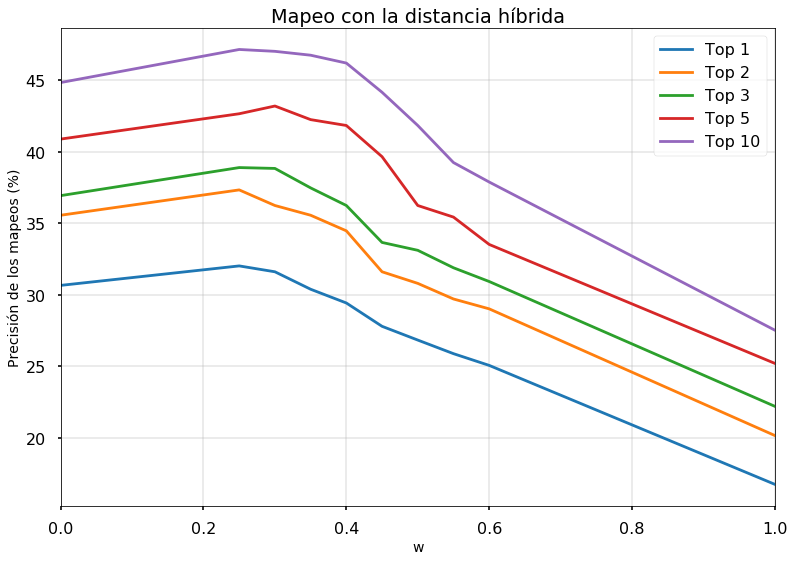
\includegraphics[width=0.8\textwidth]{imagenes/resultados/plot/rr.png}
    \caption{Medida de distancia híbrida: comportamiento del parámetro w }
    \label{fig:plot_w}
\end{figure}


\subsubsection{Medidas de distancia difusas}

Tal y como se ha podido ver en los resultados alcanzados con las métricas anteriores, se hace necesario involucrar otras técnicas que permitan un tratamiento de la información textual capaz de lidiar con distintos niveles de detalle en las descripciones, así como con la ambigüedad intrínseca del lenguaje para poder llevar a cabo un procedimiento de mapeo más robusto. En este caso, tal y como se comentó previamente, se han obtenido versiones difusas de Jaccard y de Word Mover's. 

\begin{flushleft}
   \textit{Jaccard difuso}
\end{flushleft}
% \subsubsection{Jaccard difuso}

Como se ha podido observar en la Tabla \ref{table8}, los resultados obtenidos con la medida de Jaccard difusa mejoran los conseguidos con la versión clásica, debido a una mayor permisividad al considerar que los elementos que se comparen no tienen por qué ser exactamente iguales a la hora de detectar equivalencias (aunque sí suficientemente parecidos). Sin embargo, a pesar de obtener mejores resultados que con la distancia de Jaccard, sigue habiendo una fuerte dependencia entre el parecido de palabras concretas entre las descripciones, como se puede apreciar en la fila (4) en la Tabla \ref{table:jac_fuzzy}, que muestra algunos de los mapeos obtenidos con la medida difusa de Jaccard. Esto es debido en su mayoría a las implicaciones que conlleva trabajar con descripciones sintácticas a la hora de detectar posibles equivalencias.

\setlength{\tabcolsep}{2pt} 
\begin{table}[H]
\begin{tabular}{p{0.035\textwidth}p{0.24\textwidth}|p{0.26\textwidth}|p{0.27\textwidth}|p{0.10\textwidth}p{0.01\textwidth}}
& \textbf{Alimento a \newline mapear (i-Diet)} & \textbf{Alimento mapeado (USDA)} & \textbf{Mejor mapeo\newline posible (USDA)} & \textbf{Valor\newline distancia} &  \\ \hline

(1) & Avocado & Avocado, raw & Avocado, raw & 0.5 & \textcolor{myGreen}{\cmark} \\ 

(2) & Watercress & Watercress, raw & Watercress, raw & 0 & \textcolor{myGreen}{\cmark} \\

(3) & Crab & Crab, cooked, NS as to cooking method & Crab, cooked, NS as to cooking method & 0.333 & \textcolor{myGreen}{\cmark} \\

(4) & Soybean sprouts & Sprouts, NFS & Bean sprouts, raw & 0.666 & \textcolor{myRed}{\xmark} \\

(5) & Broccoli & Licorice & Broccoli, raw & 0.16 & \textcolor{myRed}{\xmark} \\

(6) & Peanut, roasted & Peanuts, honey roasted & Peanuts, roasted, salted & 0.333 & \textcolor{myRed}{\xmark} \\

\end{tabular}
\caption{\label{table:jac_fuzzy} Resultados obtenidos con la distancia de Jaccard difusa}
\end{table}



\begin{flushleft}
    \textit{Distancia difusa entre documentos}
\end{flushleft}
% \subsubsection{Distancia difusa entre documentos}

En vista a los resultados obtenidos con esta medida de distancia (ver Tabla \ref{table8}), con esta medida es con la que alcanzamos los mejores resultados. Esto se debe mayoritariamente a que con las medidas detalladas hasta ahora, se le da mucha importancia a cada elemento considerado dentro de la descripción, ya que todas las palabras tienen la misma importancia en la descripción global. Sin embargo, si nos referimos al procesamiento de lenguaje natural, suponer que cada elemento de la descripción tiene la misma relevancia no es una buena práctica, ya que favorece a evaluar la similitud entre descripciones valorándola elemento a elemento y no como un todo. Con esta métrica le estamos dando mayor importancia al conjunto en sí, puesto que a la hora de calcular el papel que tiene cada elemento en la descripción, lo hacemos en función de su parecido semántico con la otra descripción a un nivel global. Con ello, permitimos una mayor flexibilidad a la hora de encontrar equivalencias en la base de datos. 


Resultados concretos con esta medida de distancia se pueden ver en la Tabla \ref{table:ddd}. En términos generales, se puede observar cómo se obtiene mayor rigor con esta técnica, pues mejora mapeos erróneos vistos en apartados anteriores (como en las filas 1 y 5). Además, se ha observado un comportamiento generalizado en las correspondencias obtenidas, y es que mantiene la semántica de los elementos a mapear. Con ello nos referimos a que con la semántica capturada con el modelo somos capaces de identificar los alimentos a nivel de ingrediente o alimento principal en la descripción y las dificultades que obtenemos se deben en su mayoría a los problemas derivados de distintos niveles de detalle entre ambas bases de datos. Esto es lo ocurre con el mapeo (4) y (5) en la Tabla \ref{table:ddd}. Esto último es relevante en nuestro problema a resolver, puesto que esta semántica intrínseca nos permitirá detectar alimentos equivalentes entre sí cuando queramos modificar alimentos concretos de las recetas.


    
\setlength{\tabcolsep}{2pt} 
\begin{table}[H]
\begin{tabular}{p{0.035\textwidth}p{0.24\textwidth}|p{0.26\textwidth}|p{0.27\textwidth}|p{0.10\textwidth}p{0.01\textwidth}}
& \textbf{Alimento a \newline mapear (i-Diet)} & \textbf{Alimento mapeado (USDA)} & \textbf{Mejor mapeo\newline posible (USDA)} & \textbf{Valor\newline distancia} &  \\ \hline

(1) & Sausage Bratwurst & Bratwurst & Bratwurst & 0.5 & \textcolor{myGreen}{\cmark} \\ 

(2) & Chicory & Chicory beverage & Chicory beverage & 0.285 & \textcolor{myGreen}{\cmark} \\

(3) & Chocolate and cream pudding, Chamburcy & Pie, chocolate cream & Pie, chocolate cream & 0.555 & \textcolor{myGreen}{\cmark} \\

(4) & Swett potatoes & Potato, NFS & Sweet potato NFS & 0.0 & \textcolor{myRed}{\xmark} \\

(5) & Cocoa and hazelnut butter, Nocilla, Nutela & Hazelnuts & No matches & 0.8 & \textcolor{myRed}{\xmark} \\

(6) & Sobrasada mallorquina & No matches & No matches & $\infty$ & \textcolor{myRed}{\xmark} \\

\end{tabular}

\caption{\label{table:ddd} Resultados obtenidos con la distancia entre documentos difusos}
\end{table}

Por último, respecto a los valores de precisión obtenidos con esta métrica (ver \ref{table8}), debemos tener en cuenta que los resultados son de suficientemente calidad y coherencia teniendo en cuenta que el modelo de procesamiento de lenguaje natural utilizado se basa en aprendizaje predictivo no supervisado. Para comprender la calidad de los resultados obtenidos, hay que valorar que el procedimiento de mapeo obtiene para cada uno de los elementos de i-Diet, el mejor mapeo posible de entre todos los elementos en USDA (un total de 8606), realizando el cálculo de distancia para todos los posibles emparejamientos. Si nos fijamos en las columnas \textit{Top 10}, estas demuestran la tendencia a que a mayor flexibilidad en la medida de precisión utilizada seguimos siendo capaces de encontrar mapeos adecuados, y que el acierto en el mapeo no es fruto del azar. 

\subsubsection{Comparativa entre medidas difusas y no difusas}

Tal y como se observó anteriormente, los mapeos obtenidos con las medidas de distancia Jaccard y Word's Mover son mejorados por sus respectivas versiones difusas (ver Tabla \ref{table8}).

Si nos centramos exclusivamente en el caso de Jaccard, esta mejora se debe principalmente a que los mapeos obtenidos con la medida clásica de Jaccard se basan en la comparación íntegra de las descripciones desde un punto de vista morfológico. Con su versión difusa se valoran las descripciones con un mayor grado de flexibilidad, permitiendo así que el alimento principal que aparece en las descripciones se mantenga en los mapeos resultantes. Este hecho se puede apreciar en la Tabla \ref{tab:crisp-fuzzy-jaccard}, la cual recoge una comparativa de algunos mapeos obtenidos con ambas versiones (Jaccard y Jaccard difuso). En dicha tabla podemos ver cómo en las correspondencias obtenidas con la versión difusa se mantiene el concepto de \textit{Aceite}. Sin embargo, con la versión clásica de Jaccard, se tiende a proporcionar un mapeo con el ingrediente mayoritario, lo cual no tiene que derivar en un mapeo correcto (que en este caso, sería el vegetal del que se obtiene dicho aceite).

\begin{table}[H]

\begin{tabular}[c]{p{0.02\textwidth}|p{0.17
\textwidth}|p{0.17\textwidth}|p{0.20\textwidth}|p{0.17\textwidth}|p{0.18\textwidth}p{0.01\textwidth}}
 & \textbf{Alimento a} \newline \textbf{mapear (i-Diet)} & \begin{tabular}[c]{@{}l@{}}\\\textbf{Top 1} \end{tabular} &  \begin{tabular}[c]{@{}l@{}}\\\textbf{Top 2} \end{tabular} &  \begin{tabular}[c]{@{}l@{}}\\\textbf{Top 3} \end{tabular} & \textbf{Mejor mapeo posible (USDA)} & \\ \hline

$J$ & Peanut oil & Peanut oil & Peanut, boiled & Tuna pot pie & Peanut oil & \textcolor{myGreen}{\cmark} \\

$\tilde{J}$ & Peanut oil & Peanut oil & Walnut oil & Flaxseed oil & Peanut oil & \textcolor{myGreen}{\cmark} \\ \hline

$J$ & Wheat germ oil & Wheat germ oil & Wheat germ, plain & Roll, whole grain white & Wheat germ oil & \textcolor{myGreen}{\cmark} \\

$\tilde{J}$ & Wheat germ oil &  Wheat germ oil & Sunflower oil & Sesame oil & Wheat germ oil  & \textcolor{myGreen}{\cmark} \\ \hline

$J$ & Sunflower oil & Sunflower oil & Sunfloweer seeds, NFS, & Safflower oil & Sunflower oil & \textcolor{myGreen}{\cmark} \\

$\tilde{J}$ & Sunflower oil & Sunflower oil & Soybean and sunflower oil & Canola,\newline soybean and sunflower oil & Sunflower oil & \textcolor{myGreen}{\cmark} \\

\end{tabular}
\caption{\label{tab:crisp-fuzzy-jaccard} Comparación entre Jaccard ($J$) y Jaccard difuso ($\tilde{J}$) }
\end{table}


En el caso de Word Mover's, debemos valorar que la métrica computa la distancia de cada elemento en una descripción hacia el elemento más parecido en la otra descripción. Con la versión difusa que hemos diseñado inspirándonos en esta medida, valoramos el parecido de cada elemento al conjunto de la intersección generado por ambas descripciones. Esto nos permite valorar la distancia de los elementos hacia descripciones completas, para así valorar las ambigüedades y características propias del lenguaje natural presentes en ellas. En la Tabla \ref{tab:crisp-fuzzy-documents} se puede apreciar el efecto de considerar la descripción de forma más global. En los ejemplos de dicha tabla, se puede ver cómo los mapeos alcanzados con la medida de distancia difusa entre documentos ($\tilde{D}$) proporciona resultados de más calidad.








\begin{table}[H]

\begin{tabular}[c]{p{0.1\textwidth}|p{0.14
\textwidth}|p{0.17\textwidth}|p{0.20\textwidth}|p{0.17\textwidth}|p{0.15\textwidth}p{0.01\textwidth}}
 & \textbf{Alimento} \newline \textbf{amapear\newline
 (i-Diet)} & \begin{tabular}[c]{@{}l@{}}\\\textbf{Top 1} \end{tabular} &  \begin{tabular}[c]{@{}l@{}}\\\textbf{Top 2} \end{tabular} &  \begin{tabular}[c]{@{}l@{}}\\\textbf{Top 3} \end{tabular} & \textbf{Mejor mapeo posible (USDA)} & \\ \hline

$WMD$ & Cherry & Chips, rice & Cherries, dried & Ceviche & Cherry & \textcolor{myRed}{\xmark} \\

$\tilde{D}$ & Cherry & Cherries, frozen & Cherries, dried & Cobbler, cherry & Cherry & \textcolor{myGreen}{\cmark} \\ \hline

$WMD$ & Garlic & Garlic, raw & Roll, garlic & Garlic, sauce & Garlic, raw & \textcolor{myGreen}{\cmark} \\

$\tilde{D}$ & Garlic & Garlic, sauce & Garlic, sauce & Garlic, cooked & Garlic, raw & \textcolor{myRed}{\xmark} \\ \hline

$WMD$ & Lemon & Lo mein,\newline NFS & Salmon, smoked & Lo mein, with beef   & Lemon, raw & \textcolor{myRed}{\xmark} \\

$\tilde{D}$ & Lemon   & Lemon, raw & Cassaba melon, raw & Lemon butter sauce & Lemon, raw & \textcolor{myGreen}{\cmark} \\

\end{tabular}
\caption{\label{tab:crisp-fuzzy-documents} Comparación entre Word Mover's (\textit{WMD}) y Distancia difusa entre documentos ($\tilde{D}$) }
\end{table}


\subsubsection{Otras medidas de distancia}

% Se han hecho experimentos adicionales 
% Se han utilizado otras medidas de distancia pero no han funcionado y por eso no se entra en detalle. 
Además de las medidas de distancia ya comentadas en esta sección, también se hecho experimentos adicionales con otras medidas de distancia. Este es el caso de la medida de distancia sintáctica Levenshtein, así como otras pruebas híbridas combinando las medidas difusas. Con estas métricas, no se han obtenido resultados relevantes que añadan detalles adicionales a lo explicado en apartados anteriores, por lo que no se entra en detalle en este capítulo.

\subsubsection{Influencia del Word Embedding utilizado}\label{WordEmbedding}

Los resultados obtenidos con el procedimiento de mapeo también nos pueden ayudar a analizar la eficacia de utilizar un Word Embedding específico para este problema y no uno genérico ya entrenado (tal y como se mostró en el Capítulo \ref{ch:Capitulo 5}). En la Tabla \ref{tablecomp} se muestra el porcentaje de acierto de los mapeos obtenidos con un modelo de Word Embedding específico (el entrenado por nosotros) y uno genérico (un modelo de Word Embedding entrenado con el conjunto de datos de Google News). Para ello, se ha utilizado la medida de distancia con mejor comportamiento (distancia de documentos difusos). 

\setlength{\tabcolsep}{4pt} 
\begin{table}[H]
\centering
\begin{tabular}{l|l|l|l|l|l}
\textbf{Modelo de W.E.} & \textbf{Top 1} &\textbf{Top 2}& \textbf{Top 3} & \textbf{Top 5} & \textbf{Top 10}\\ \hline
W.E. Google & 5.85 & 6.26 & 6.40 & 7.22 & 7.76 \\
W.E. Recetas & 35.55 & 40.46 & 43.46 & 47.00 & 53.26 \\ 
\end{tabular}
\caption{Resultados del mapeo ($\%$) para distintos modelos de W.E.}\label{tablecomp}
\end{table}


En la Figura \ref{fig:comp} se pueden ver los resultados de la Tabla \ref{tablecomp}. Con ella, podemos ratificar que el uso de un modelo específico en este problema es lo que nos ha llevado a obtener buenas representaciones (y por tanto mapeos) que no podríamos haber obtenido con uno genérico.

\begin{figure}[H]
    \centering
    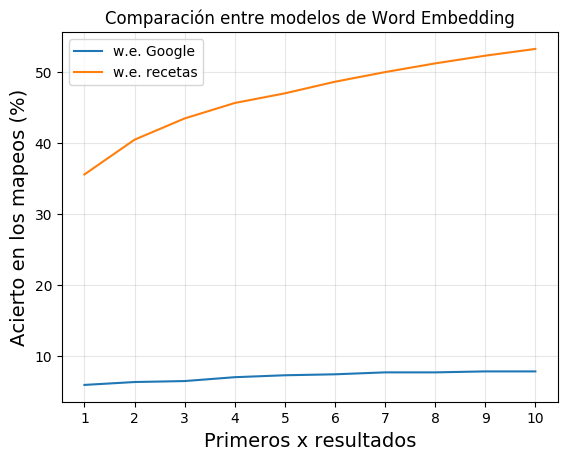
\includegraphics[width=0.80\textwidth]{imagenes/resultados/plot/xx.png}
    \caption{Comparación entre Word Embedding genéricos y preentrenados}
    \label{fig:comp}
\end{figure}




\section{Resultados del Módulo de Consultas Adaptadas}\label{sec:res_adap}

Para poder analizar los resultados obtenidos con este módulo, en este apartado se muestran algunos ejemplos representativos de adaptaciones de recetas visualizadas a través del prototipo de la aplicación. En primer lugar, vamos a ver cómo se comporta el sistema de adaptación de recetas con las restricciones incorporadas en el sistema. Para ello, se va a ilustrar con una receta cuyos ingredientes no satisfacen ni la dieta vegetariana ni la vegana (ver Figura \ref{fig:ejemplo8}). Tal y como se muestra en la Figura \ref{fig:ejemplo7}, el módulo de Consultas Adaptadas es capaz de detectar aquellos ingredientes no aptos para una dieta vegetariana (en este caso, el ingrediente \textit{Bacon)}. De igual forma ocurre con la opción vegana, cuyos ingredientes no veganos son detectados también a través del módulo de Consultas Adaptadas (ver Figura \ref{fig:ejemplo6}).


\begin{figure}[H]
    \centering
    \begin{subfigure}[b]{0.31\linewidth}
        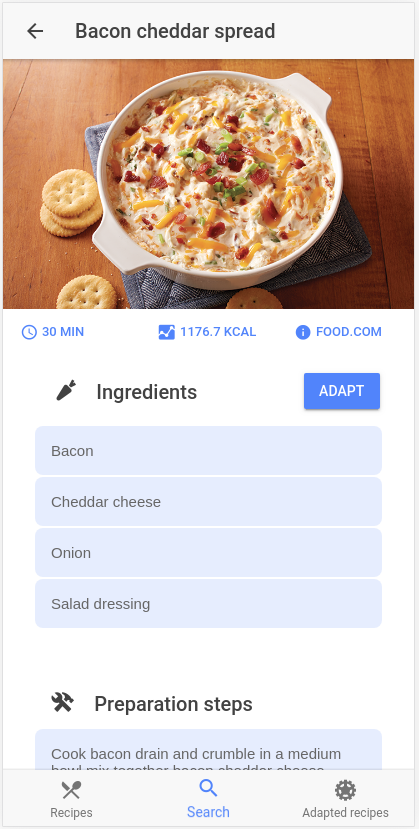
\includegraphics[width=\linewidth]{imagenes/app/pantallas/ejemplo8.png}
        \caption{Receta original}
        \label{fig:ejemplo8}
    \end{subfigure}
    \begin{subfigure}[b]{0.308\linewidth}
        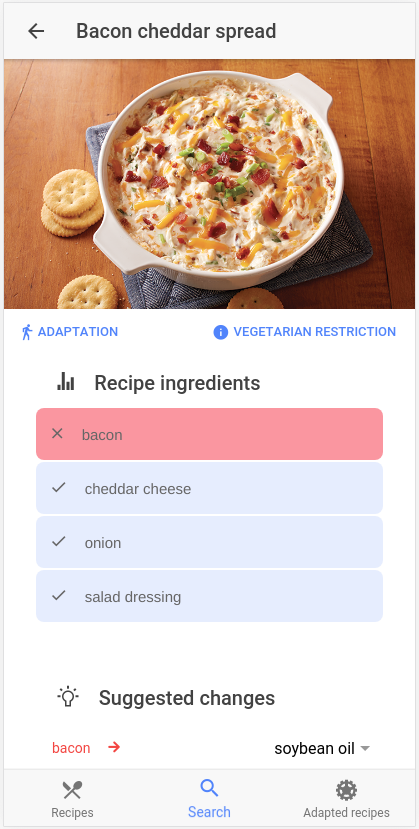
\includegraphics[width=\linewidth]{imagenes/app/pantallas/ejemplo7.png}
        \caption{Opción vegetariana}
        \label{fig:ejemplo7}
    \end{subfigure}
    \begin{subfigure}[b]{0.31\linewidth}
        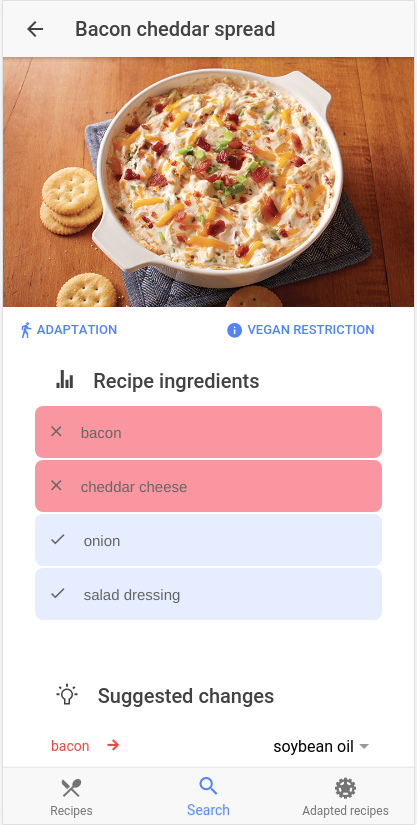
\includegraphics[width=\linewidth]{imagenes/app/pantallas/ejemplo6.png}
        \caption{Opción vegana}
        \label{fig:ejemplo6}
    \end{subfigure}
    \caption{Adaptación de recetas a restricciones vegetarianas y veganas}
    \label{fig:todos}
\end{figure} 

Si nos centramos en adaptaciones a dietas veganas, en la Figura \ref{fig:ejemplo1} se puede ver una receta con ingredientes no compatibles con dicha dieta. De hecho, al aplicar la restricción de dieta vegana (ver Figura \ref{fig:ejemplo2}), podemos ver cómo el sistema evalúa correctamente los ingredientes al detectar aquellos no compatibles con la restricción. Si modificamos el ingrediente no compatible (en este caso es \textit{Mantequilla}), se facilitan algunas alternativas para poder sustituir dicho ingrediente. Podemos observar en la Figura \ref{fig:ejemplo3} algunas de las opciones para reemplazar la mantequilla: entre ellas, se propone la mantequilla vegetal, la cual es apta para estas dietas. Sin embargo, no siempre obtenemos adaptaciones adecuadas para las recetas. Un ejemplo de ello ocurre con la receta mostrada en la Figura \ref{fig:ejemplo10}. Tal y como se detecta con el módulo de Consultas Adaptadas, esta receta contiene \textit{Leche}, ingrediente no apto para una receta vegana (ver Figura \ref{fig:ejemplo11}). Sin embargo, ninguna las alternativas propuestas es adecuada para la receta en cuestión (ver Figura \ref{fig:ejemplo12}). Esto se debe a que no siempre se consigue un alimento alternativo totalmente adecuado para la receta, más aún si se trata de restricciones tan estrictas que limitan los alimentos permitidos a un conjunto muy escaso que impide encontrar opciones que mantengan la esencia del plato.


\begin{figure}[H]
    \centering

    \begin{subfigure}[b]{0.30\linewidth}
        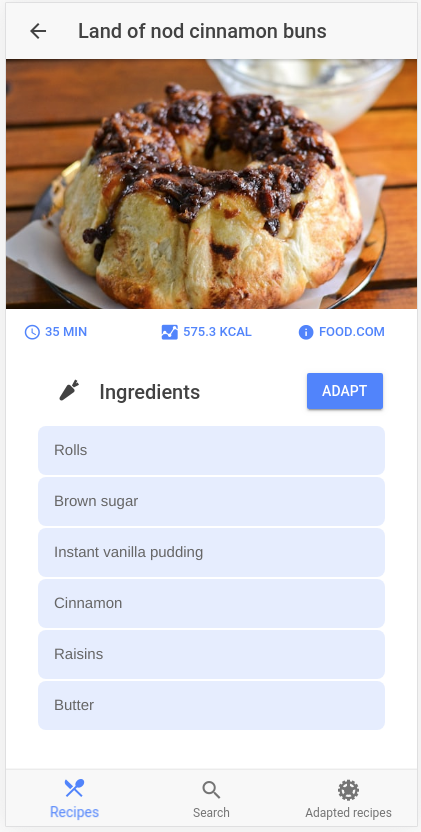
\includegraphics[width=\linewidth]{imagenes/app/pantallas/ejemplo1.png}
        \caption{Receta original}
        \label{fig:ejemplo1}
    \end{subfigure}
    \begin{subfigure}[b]{0.303\linewidth}
        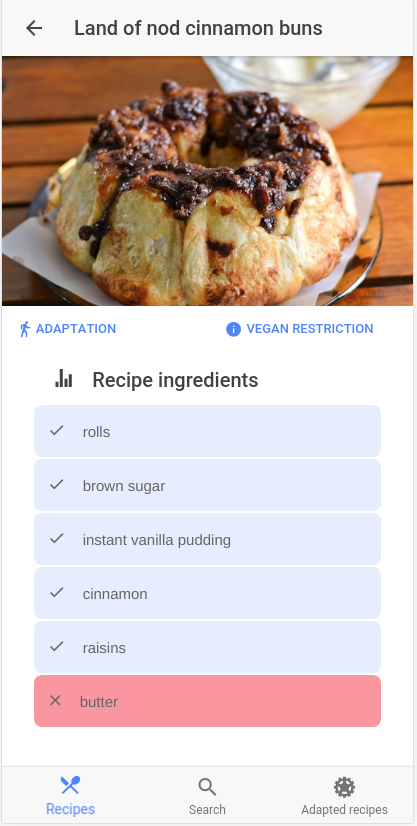
\includegraphics[width=\linewidth]{imagenes/app/pantallas/ejemplo2.png}
        \caption{Adaptando receta I}
        \label{fig:ejemplo2}
    \end{subfigure}
    \begin{subfigure}[b]{0.30\linewidth}
        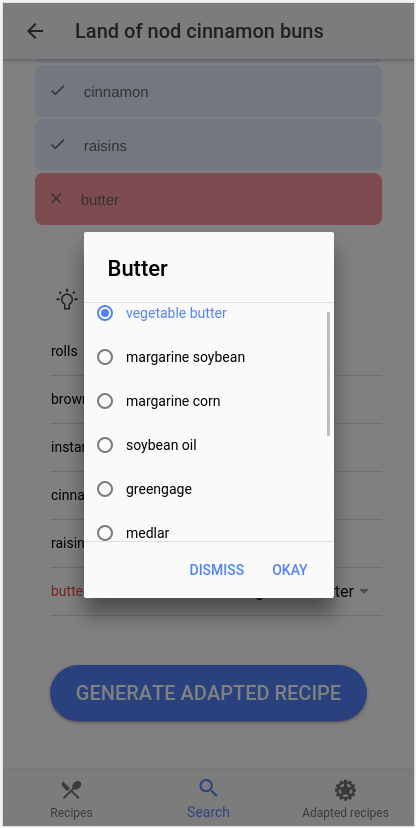
\includegraphics[width=\linewidth]{imagenes/app/pantallas/ejemplo3.png}
        \caption{Adaptando receta II}
        \label{fig:ejemplo3}
    \end{subfigure}
    \caption{Adaptación de una receta vegana I}
    \label{fig:seleccion1}
\end{figure} 

\begin{figure}[H]
    \centering
    \begin{subfigure}[b]{0.30\linewidth}
        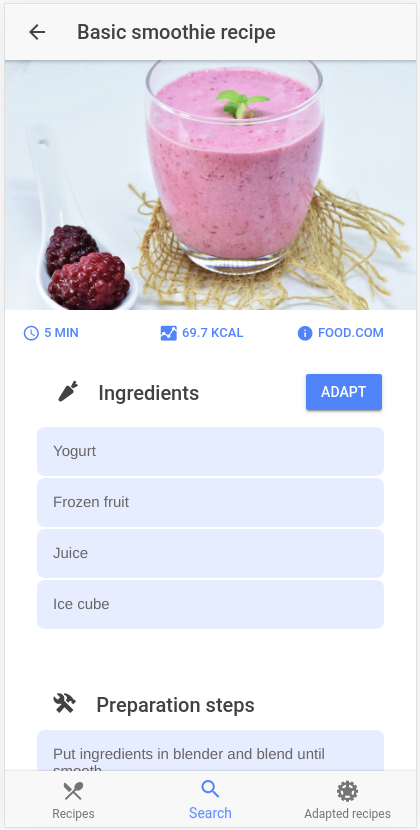
\includegraphics[width=\linewidth]{imagenes/app/pantallas/ejemplo10.png}
        \caption{Receta original}
        \label{fig:ejemplo10}
    \end{subfigure}
    \begin{subfigure}[b]{0.301\linewidth}
        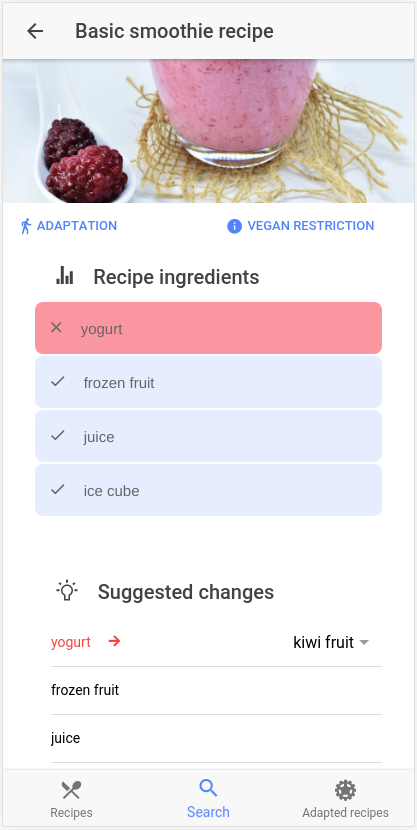
\includegraphics[width=\linewidth]{imagenes/app/pantallas/ejemplo11.png}
        \caption{Adaptando receta I}
        \label{fig:ejemplo11}
    \end{subfigure}
    \begin{subfigure}[b]{0.299\linewidth}
        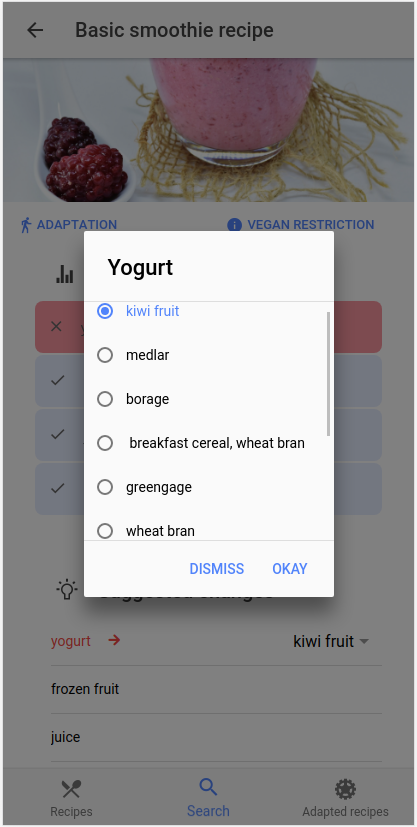
\includegraphics[width=\linewidth]{imagenes/app/pantallas/ejemplo12.png}
        \caption{Adaptando receta II}
        \label{fig:ejemplo12}
    \end{subfigure}
    \caption{Adaptación de una receta vegana II}
    \label{fig:seleccion3}
\end{figure}


Por último, en las Figuras \ref{fig:ejemplo13}, \ref{fig:ejemplo14} y \ref{fig:ejemplo15} se muestra un ejemplo de adaptación sujeta a las restricciones de la
receta vegetariana. Se puede ver que los elementos que se deben adecuar a dicha dieta son       detectados correctamente (en este caso el ingrediente \textit{Pollo)}, y algunas de las sugerencias para su sustitución. Se puede apreciar que las alternativas son coherentes, puesto que se sugiere utilizar verdura o incluso algún tipo de fruta en su lugar, los cuales son substitutos bastante intuitivos para esta dieta.

\begin{figure}[H]
    \centering
    \begin{subfigure}[b]{0.31\linewidth}
        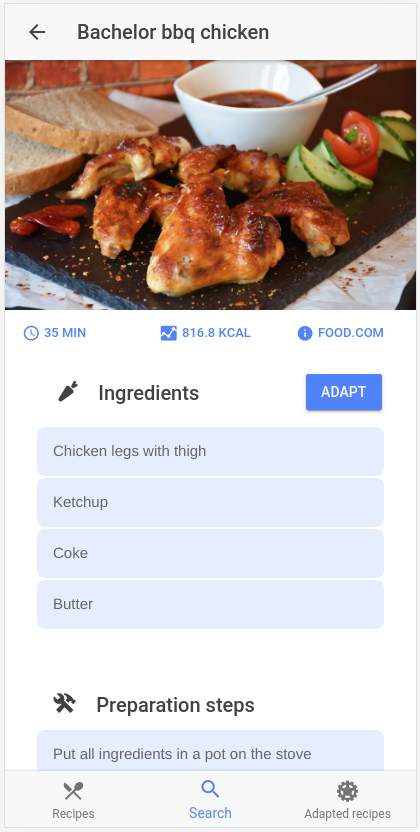
\includegraphics[width=\linewidth]{imagenes/app/pantallas/ejemplo13.png}
        \caption{Receta original}
        \label{fig:ejemplo13}
    \end{subfigure}
    \begin{subfigure}[b]{0.31\linewidth}
        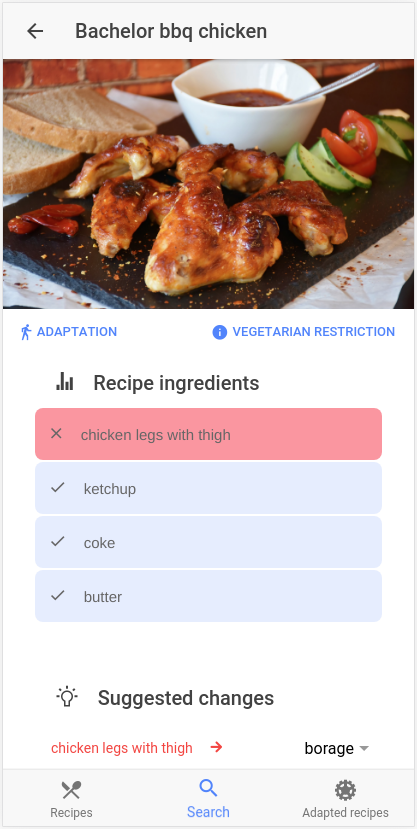
\includegraphics[width=\linewidth]{imagenes/app/pantallas/ejemplo14.png}
        \caption{Adaptando receta I}
        \label{fig:ejemplo14}
    \end{subfigure}
    \begin{subfigure}[b]{0.31\linewidth}
        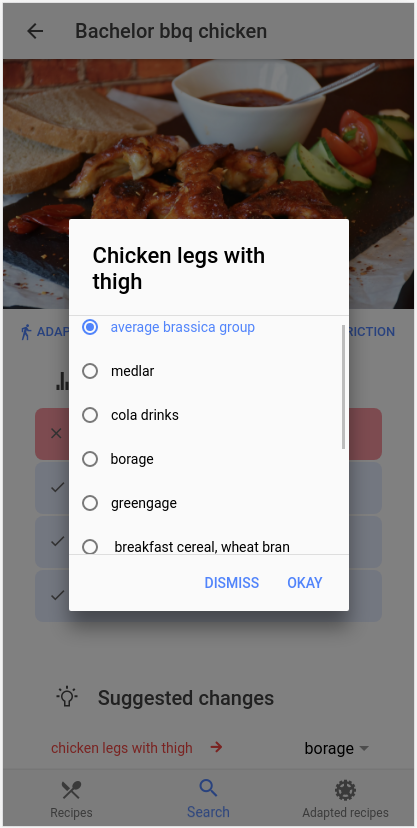
\includegraphics[width=\linewidth]{imagenes/app/pantallas/ejemplo15.png}
        \caption{Adaptando receta II}
        \label{fig:ejemplo15}
    \end{subfigure}
    \caption{Adaptación de una receta vegetariana}
    \label{fig:seleccion2}
\end{figure}

% Con los ejemplos mostrados en este apartado hemos podido comprobar las ventajas de utilizar el modelo predictivo implementado para poder adaptar dietas, puesto que la semántica capturada en el modelo permite alcanzar buenas alternativas a los elementos restringidos. Por otra parte, se ha podido ver la interpretabilidad de este módulo, ya que paso a paso se indican aquellos ingredientes no adecuados y que deben ser sustituidos por otros. 

\chapter{Conclusiones}
\label{ch:Conclusiones}

\begin{quote}
  Este capítulo recoge los principales aspectos concluidos del desarrollo del documento y las futuras líneas de trabajo con las que continuar este proyecto.
\end{quote}


\section{Conclusiones}


% Con la app desarrollada no sólo se puede ver el alcance de la herramienta, sino que se ha podido aplicar a un problema de relevancia que permite ver la gran utilidad que tiene este tipo de herramientas. ( Apartado 4.2.3 )

%  Esto se debe a que esta herramienta se implementa de forma independiente al problema que se intenta resolver con dichos datos, dando lugar a su aplicación en múltiples campos. ( Apartado 4.2.3 ) generalizable a otros campos de estudio. 

Con las representaciones obtenidas con el modelo de Word Embedding entrenado en este trabajo hemos podido ver que utilizar técnicas predictivas de este tipo para obtener representaciones textuales nos ha permitido capturar la semántica de la terminología alimenticia, dando lugar a aproximaciones más precisas que nos permitan tratar con problemas comunes en el lenguaje culinario, como el uso de marcas y sinónimos alimenticios. Al contrario que en otros modelos de Word Embedding en Food Computing, en nuestro caso no sólo utilizamos los ingredientes de las recetas, también usamos el texto que describe las instrucciones de cocción para el entrenamiento del modelo. Con ello, conseguimos obtener codificaciones cercanas para los ingredientes que aparecen juntos en las recetas, pero también para aquellos que están involucrados en preparaciones similares. Esto es útil para la comparación de elementos a nivel multicultural, y también para detectar posibles alternativas o substitutos de alimentos en base a las instrucciones de cocinado empleadas en las recetas. Sin embargo, es importante tener en cuenta que al estar utilizando recetas en el corpus de entrenamiento, corremos el riesgo de obtener muy buenas representaciones de alimentos con mucho protagonismo en el mundo culinario pero pobres o incluso inexistentes para aquellos elementos que no suelan aparecer en las recetas de este tipo de páginas web. Además, es importante valorar que, en este tipo de bases de datos nutricionales, se tienen en cuenta especies florales que no suelen ser consumidas por la población: con nuestro conjunto de entrenamiento, no seríamos capaz de obtener representaciones para este tipo de elementos. Por ello, un conjunto de entrenamiento más amplio, capaz de abarcar alimentos más allá de las recetas, podría subsanar este posible sesgo introducido en el modelo. 

Como se ha podido comprobar con las experimentaciones realizadas, las consideraciones tenidas en cuenta al definir medidas que permitan detectar equivalencias cambian totalmente el comportamiento del módulo de mapeo. Por ello, se han valorado distintos enfoques abarcando tanto información sintáctica y semántica como la vaguedad en el lenguaje que pueda existir en las fuentes de datos utilizadas. Aun así, la similitud entre textos cortos sigue siendo un desafío debido a la dificultad añadida de tratar con su breve contenido, donde se incrementa mucho la importancia que tiene cada palabra perteneciente a la descripción. A pesar de que la información sintáctica y semántica tienen relevancia en este punto (y deben ser tenidas en cuenta en los mapeos) el uso de una métrica que permita darle más importancia a la descripción en sí que a los elementos concretos que forman parte de la misma ha sido determinante para ser capaces de detectar equivalencias entre las bases de datos. No obstante, en los casos de mapeos incorrectos, los resultados han seguido mostrando la calidad y robustez de la herramienta, permitiendo detectar buenas aproximaciones e ingredientes principales. Por otra parte, al analizar los mejores posibles mapeos para cada elemento de i-Diet, hemos podido darnos cuenta cómo no sólo el mejor mapeo posible es de calidad, sino que las 10 primeras alternativas siguen mostrando una mejora muy sustancial en los resultados. Estos mejores mapeos obtenidos con nuestra estrategia, podrían ser combinados con otro tipo de técnicas, o incluso enriquecidos con mayor información del conjunto de datos con el objetivo de alcanzar resultados más exactos.

Con el prototipo implementado para la aplicación de recetas adaptadas hemos podido ver la potencia que podría tener esta aplicación más allá de una solución a un problema de mapeo. Se han podido ver las ventajas de utilizar el modelo predictivo implementado para poder adaptar dietas, puesto que la semántica capturada en el modelo permite alcanzar buenas alternativas a los elementos restringidos. Por otra parte, se ha permitido ver la interpretabilidad de este módulo, ya que paso a paso se indican aquellos ingredientes no adecuados y que deben ser sustituidos por otros. Esta interpretabilidad nos ha permitido percartarnos de la dificultad de algunas adaptaciones, en las que las restricciones limitan las posiblidades de mapeo a alimentos que son difícilmente combinables con los ingredientes de la receta. Esto no deja de ser un problema fuera del ámbito de la computación, ya que la versión vegana o vegetariana de un plato no tiene por qué ser una solución intuitiva de por sí.

En los capítulos correspondientes a cada uno de los módulos implementados, así como en la experimentación llevada a cabo con ellos, se ha podido apreciar que se han tenido en cuenta con éxito los requisitos definidos en el Capítulo \ref{ch:Capitulo 2}. Sin embargo, dada la etapa de desarrollo en la que se encuentra la aplicación móvil (como comentamos en el Capítulo \ref{ch:Consultas_Adaptadas} se trata de un prototipo funcional), el nivel de cumplimiento de los requerimientos relativos a la interfaz podría mejorarse con la realimentación que se obtiene de las pruebas y evaluación con usuarios en etapas posteriores de desarrollo.

Por último, puntualizar que las distintas tareas de Food Computing involucradas en el problema que hemos abordado en este trabajo (Predicción, Recomendación, Identificación y Recuperación de información) son tareas generales que se pueden encontrar en otros campos de estudio que no tienen por qué estar centrados en el ámbito culinario y de la nutrición. Al tratarse de tareas comúnmente abordadas en cualquier campo, justifican aún más la independencia del sistema desarrollado al área de Food Computing, posibilitando su aplicación en otros muchos contextos. Con ello, queremos destacar la relevancia de esta aproximación para resolver problemas que lidien con información heterogénea, puesto que todo el procedimiento puede ser aplicable a otro campo de estudio, cambiando las fuentes de datos y  el modelo de Word Embedding por uno específico en el área en cuestión o incluso por uno genérico si la situación lo propiciase.


\section{Trabajo futuro}

A lo largo del trabajo, hemos podido ver las grandes posibilidades que brindan los modelos predictivos a la hora de trabajar con modelos de lenguaje. En este punto se abren nuevas vías que pretendemos estudiar para poder obtener un modelo del lenguaje más sofisticado. 
Como es de esperar en un problema de predicción, una vía de mejora reside en la calidad de los datos utilizados. Las dificultades que nos hemos encontrado a causa de traducciones inexactas e incorrectas en los datos han derivado en representaciones del lenguaje imprecisas. Una mejora de las traducciones de los alimentos, así como de errores tipográficos, permitiría reducir el ruido añadido, y obtener mejores resultados: cuanta mayor calidad tengan los datos textuales con los que trabajemos, con mayor facilidad encontraremos buenas representaciones con el modelo. Por ello, también planteamos el uso de técnicas de Traducción Automática (Machine Translation) para mejorar la calidad de estos y así reducir el ruido añadido en los datos. Además, aumentar la cantidad de datos alimenticios abarcados en el conjunto de entrenamiento para el Word Embedding nos permitirá obtener un vocabulario más amplio. Para ello, estudiaremos obtener un corpus de entrenamiento más extenso más allá de la información que nos puedan proporcionar las recetas, para así poder recoger tanto vocabulario alimenticio como nos sea posible. Además de aumentar el tamaño del corpus de entrenamiento, como trabajo futuro se plantea utilizar otros modelos de lenguaje más actuales como BERT~\cite{devlin2018bert}, así como aplicar Trasferencia de Aprendizaje~\cite{pan2009survey} (Transfer Learning) con el modelo ya implementado con el objetivo de obtener representaciones aún más precisas que nos permitan convertir los mapeos aproximados (aunque erróneos) en correctos.

Por otra parte, trabajar con modelos de Word Embedding en Food Computing nos ha llevado a comprobar la importancia de la influencia cultural existente al utilizar las distintas cocinas del mundo. Esta dificultad abre nuevas vías de estudio con modelos de lenguaje en Food Computing, tales como abordar problemas de modelos de Word Embedding multilingües, más conocidos como \textit{Cross-Lingual Word Embedding}~\cite{ruder2019survey} en vistas a poder lidiar de forma más sofisticada con las características culturales contenidas en los datos con los que hemos trabajado en este proyecto. Con ello, podríamos detectar posibles transformaciones lineales de los datos alimenticios entre zonas geográficas y abordar de forma más sofisticada las dificultades intrínsecas al trabajar con bases de datos nutricionales procedentes de distintas culturas.

A su vez, confiamos en que transformar este problema en uno multimodal que tenga en cuenta el resto de información contenida acerca de cada alimento (como puede ser el grupo de alimento o incluso los macronutrientes) nos permita obtener un procedimiento de mapeo más robusto, así como una mayor precisión en los resultados. La información que acompaña a los alimentos nos puede ayudar a mejorar la calidad de los mapeos, ya que estaríamos teniendo en cuenta descripciones más completas de los elementos a mapear. Para ello, pretendemos estudiar el problema desde dos perspectivas: en primer lugar, considerar un modelo predictivo que combine la representación vectorial de las descripciones con el resto de datos asociados a cada elemento; y en segundo lugar, considerar estos datos adicionales a la descripción textual en la función de distancia utilizada para medir la similitud entre los alimentos. 
 


\printbibliography %Prints bibliography
%%\chapter{Conclusiones y Trabajos Futuros}
%
%

\newpage
%%\nocite{*}

% Comentadas estas tres líneas
%\addcontentsline{toc}{chapter}{Bibliografía}
%\bibliographystyle{abbrvnat}
%\bibliography{library}


\appendix
\chapter{Manual de usuario}
\label{ch:Anexo_Pantallas}

Con el inicio de la ejecución de la aplicación, aparece un tutorial introductorio que informa al usuario acerca del funcionamiento básico de ésta. Las pantallas que forman esta guía introductoria se muestran de manera ordenada en las Figuras \ref{fig:app_tutorial1}, \ref{fig:app_tutorial2}, \ref{fig:app_tutorial3} y \ref{fig:app_tutorial4}. Para navegar por cada una de estas pantallas, simplemente hay que deslizar la ventana de derecha a izquierda hasta llegar la última pantalla del tutorial, que permite acceder a la pantalla de bienvenida a través del botón \texttt{CONTINUE} (ver Figura \ref{fig:app_welcome}). El botón \texttt{SKIP} en las pantallas \ref{fig:app_tutorial1}, \ref{fig:app_tutorial2} y \ref{fig:app_tutorial3} facilita un acceso directo a la pantalla de bienvenida sin necesidad de recorrer la guía introductoria.

\begin{figure}[H]
    \centering
    \begin{subfigure}[b]{0.31
    \linewidth}
        \includegraphics[width=\linewidth]{imagenes/app/pantallas/app_tutorial1.png}
        \caption{Pantalla tutorial I}
        \label{fig:app_tutorial1}
    \end{subfigure}
    \begin{subfigure}[b]{0.31
    \linewidth}
        \includegraphics[width=\linewidth]{imagenes/app/pantallas/app_tutorial2.png}
        \caption{Pantalla tutorial II}
        \label{fig:app_tutorial2}
    \end{subfigure}
        \begin{subfigure}[b]{0.31
        \linewidth}
        \includegraphics[width=\linewidth]{imagenes/app/pantallas/app_tutorial3.png}
        \caption{Pantalla tutorial III}
        \label{fig:app_tutorial3}
    \end{subfigure}
    \caption{Pantallas de inicio a la aplicación I}
    \label{fig:pantallas_inicio1}
\end{figure}

Una vez que se pulsa el botón \texttt{LET'S COOK} en la pantalla de bienvenida, se accede a las distintas colecciones de recetas en las que se organizan las recetas (ver Figura \ref{fig:app_coleccion}). Esta pantalla se corresponde con la pantalla de inicio de la aplicación. En dicha pantalla se muestran tres pestañas en la barra inferior: \textit{Recipes} (en la que se muestra la pantalla inicial), \textit{Search} (la cual permite realizar búsquedas sobre todas las recetas de la base de datos) y \textit{Adapted Recipes}, que contiene recetas ya adaptadas que se han querido almacenar para uso posterior.

\begin{figure}[H]
    \centering
    \begin{subfigure}[b]{0.32\linewidth}
        \includegraphics[width=\linewidth]{imagenes/app/pantallas/app_tutorial4.png}
        \caption{Pantalla tutorial IV}
        \label{fig:app_tutorial4}
    \end{subfigure}
    \begin{subfigure}[b]{0.32\linewidth}
        \includegraphics[width=\linewidth]{imagenes/app/pantallas/app_welcome.png}
        \caption{Pantalla bienvenida}
        \label{fig:app_welcome}
    \end{subfigure}
        \begin{subfigure}[b]{0.32\linewidth}
        \includegraphics[width=\linewidth]{imagenes/app/pantallas/app_1.png}
        \caption{Colecciones}
        \label{fig:app_coleccion}
    \end{subfigure}
    \caption{Pantallas de inicio a la aplicación II}
    \label{fig:pantallas_inicio2}
\end{figure}

Para acceder a una receta concreta se pueden seguir dos formas: seleccionar una colección de las mostradas en la pantalla principal (ver Figura \ref{fig:app_5}) o a través de la pantalla del buscador de recetas (ver Figura \ref{fig:app_6}). Una vez que se está en la vista detallada de una receta (ver Figura \ref{fig:ejemplo1_}) ya podemos proceder a su adaptación mediante el botón azul \texttt{ADAPT}. Una vez que se indica la restricción a aplicar sobre la receta (ver Figura \ref{fig:app_7}) se facilita una pantalla intermedia que muestra la adecuación de los ingredientes a la restricción (ver Figura \ref{fig:ejemplo2_}). En esta última pantalla, se facilitan alternativas a cada ingrediente no compatible con la dieta para proceder a su modificación (ver Figura \ref{fig:ejemplo3_}). Una vez seleccionadas las alternativas a los alimentos que deben modificarse, se muestra la receta adaptada con los cambios tanto los ingredientes como los pasos de preparación que se tendrían que variar (ver Figuras \ref{fig:app_9} y \ref{fig:app_8}). 

\begin{figure}[H]
    \centering
    \begin{subfigure}[b]{0.32\linewidth}
        \includegraphics[width=\linewidth]{imagenes/app/pantallas/app_5.png}
        \caption{Recetas en colección}
        \label{fig:app_5}
    \end{subfigure}
    \begin{subfigure}[b]{0.319\linewidth}
        \includegraphics[width=\linewidth]{imagenes/app/pantallas/app_6.png}
        \caption{Buscador de recetas}
        \label{fig:app_6}
    \end{subfigure}
        \begin{subfigure}[b]{0.32\linewidth}
        \includegraphics[width=\linewidth]{imagenes/app/pantallas/ejemplo1.png}
        \caption{Vista de receta}
        \label{fig:ejemplo1_}
    \end{subfigure}
    \caption{Pantallas para adaptar recetas}
    \label{fig:pantallas_inicio3}
\end{figure}

\begin{figure}[H]
    \centering
    \begin{subfigure}[b]{0.32\linewidth}
        \includegraphics[width=\linewidth]{imagenes/app/pantallas/app_7.png}
        \caption{Adaptar receta I}
        \label{fig:app_7}
    \end{subfigure}
    \begin{subfigure}[b]{0.3235
    \linewidth}
        \includegraphics[width=\linewidth]{imagenes/app/pantallas/ejemplo2.png}
        \caption{Adaptar receta II}
        \label{fig:ejemplo2_}
    \end{subfigure}
        \begin{subfigure}[b]{0.32\linewidth}
        \includegraphics[width=\linewidth]{imagenes/app/pantallas/ejemplo3.png}
        \caption{Adaptar receta III}
        \label{fig:ejemplo3_}
    \end{subfigure}
    \caption{Pantallas de navegación de recetas}
    \label{fig:pantallas_inicio4}
\end{figure}

Finalmente, arriba a la derecha en la pantalla de la receta adaptada (ver Figura \ref{fig:app_8}) hay un botón que permite guardar la receta adaptada en una colección dedicada para ello (ver Figura \ref{fig:app_10}).

\begin{figure}[H]
    \centering
    \begin{subfigure}[b]{0.32\linewidth}
        \includegraphics[width=\linewidth]{imagenes/app/pantallas/app_8.png}
        \caption{Receta adaptada I}
        \label{fig:app_8}
    \end{subfigure}
    \begin{subfigure}[b]{0.32\linewidth}
        \includegraphics[width=\linewidth]{imagenes/app/pantallas/app_9.png}
        \caption{Receta adaptada II}
        \label{fig:app_9}
    \end{subfigure}
        \begin{subfigure}[b]{0.32\linewidth}
        \includegraphics[width=\linewidth]{imagenes/app/pantallas/app_10.png}
        \caption{Recetas adaptadas}
        \label{fig:app_10}
    \end{subfigure}
    \caption{Pantallas de la receta adaptada}
    \label{fig:pantallas_inicio5}
\end{figure}

%\input{apendices/manual_usuario/manual_usuario}
%%\input{apendices/paper/paper}
%\input{glosario/entradas_glosario}
% \addcontentsline{toc}{chapter}{Glosario}
% \printglossary
\chapter*{}
\thispagestyle{empty}




%Imports the bibliography file "references.bib"


\end{document}
